% ============================================================================
% 论文主文（预注册协议驱动，目标期刊：Physiol Meas / BSPC / CBM 中科院2区）
% 文件名: paper/main.tex
% 状态: v2.0 6方向×2架构稳健性版（基于多seed稳健性验证 + 预注册修订案A1）
% 依据: docs/EXPERIMENT_PROTOCOL.md v2.1-A1
%   - 主终点 ΔECE_OOD = ECE_raw_OOD − ECE_TS_OOD（A1.1 重新定位）
%   - 主检验 H₀: ΔECE_OOD = 0 vs H₁: ΔECE_OOD > 0（单侧，方向先验）
%   - 5 个独立贡献：OOD 收益量化 + ID 边界条件 + Shapley 分解验证 + 方法选择边界 + 判别感知校准门
%   - v2.1 更新：6方向 × 2架构（InceptionTime + ResNet1D）× 5seed = 60 实验（完整覆盖）
% 写作纪律（协议§0）：不得声称"首次证明ECG校准收益ID→OOD衰减"（Ovadia 2019
%   已知）；4 个独立贡献（OOD 收益量化 / ID 边界 / Shapley 验证 / 方法选择边界）
%   才是 novelty 核心。5 个独立贡献（OOD 收益量化 / ID 边界 / Shapley 验证 / 方法选择边界 / 判别感知校准门）5 个独立贡献（OOD 收益量化 / ID 边界 / Shapley 验证 / 方法选择边界 / 判别感知校准门）
% 透明性声明：本主检验为预注册修订案 A1 后的重新定位（exploratory + 稳健性验证），
%   非 confirmatory；修订案全文见 docs/PROTOCOL_AMENDMENT_A1_PREREG_RELOCATION.md。
% ============================================================================
\documentclass[review,12pt,nonatbib]{elsarticle}
\usepackage{amsmath,amssymb,booktabs,graphicx,multirow,array}
\usepackage{microtype}  % micro-typographic enhancements, reduces overfull boxes
\microtypesetup{expansion=false}  % disable font expansion (incompatible with elsarticle)
\usepackage[utf8]{inputenc}
\usepackage[T1]{fontenc}
\usepackage{pifont}
\usepackage{lineno}
\usepackage{hyperref}
\hypersetup{colorlinks=false,pdfborder={0 0 0},
  pdftitle={When Does Temperature Scaling Pay Off in Cross-Corpus ECG Transfer? A Multi-Seed Calibration Boundary Study},
  pdfauthor={Zero Token Lab}}

% --- Typesetting optimization ---
\emergencystretch=3em
\tolerance=2000
\hbadness=10000
\vbadness=10000
\widowpenalty=10000
\clubpenalty=10000

\journal{Biomedical Signal Processing and Control}

\title{When Does Temperature Scaling Pay Off in Cross-Corpus ECG Transfer? A Multi-Seed Calibration Boundary Study}

\author[inst1]{Zero Token Lab\corref{cor1}}
\ead{guantong490@gmail.com}
\cortext[cor1]{Corresponding author.}
\affiliation[inst1]{organization={Deployment Science Group},
  city={Shouguang}, country={China}}

\begin{document}
\begin{frontmatter}

\begin{abstract}
Temperature scaling (TS) is the default post-hoc recalibration for deep
classifiers, yet whether its in-distribution (ID) benefit transfers to
out-of-distribution (OOD) target corpora remains the central open question
for cross-institution ECG deployment. We pre-registered and ran a
multi-seed calibration boundary study on six directed cross-corpus transfer
pairs among Chapman-Shaoxing, CPSC2018+2019, and PTB-XL, with two
architectures (InceptionTime and ResNet1D (1D-ResNet-34)), five seeds
(42--46), eight recalibration methods, and a patient-level cluster paired
bootstrap (the operating CI is BCa at $B=10{,}000$, fully re-run on
the entire 60-experiment grid; earlier percentile CIs at $B=10{,}000$
in 31/60 experiments and $B=200$ in 21/60 are retained as historical
provenance, and the two CI methods agree in sign in 60/60
experiments).
The pre-registered primary endpoint is the OOD calibration benefit
$\Delta\text{ECE}_{\text{OOD}}=\text{ECE}_{\mathrm{raw}}^{\mathrm{OOD}}
-\text{ECE}_{\mathrm{TS}}^{\mathrm{OOD}}$, tested one-sided against a
registered empirical direction prior. Across 60 seed experiments (6 pairs
$\times$ 2 architectures $\times$ 5 seeds, fully balanced), TS yields a
positive OOD benefit in 51/60 cases (85.0\%): InceptionTime 27/30 (90.0\%),
ResNet1D 24/30 (80.0\%); nine counter-examples are transparently disclosed
with post-hoc mechanistic interpretations. When six experiments with
degenerate CI widths ($<3\times10^{-4}$) are excluded, the headline
count becomes 45/60 (75.0\%), so the 85.0\% rate should be read jointly
with effect sizes and CI diagnostics. The pre-registered ID boundary
criterion ($\geq$80\% of cells with 95\% CIs containing zero) is
\emph{not} met (23/60 = 38.3\% under the BCa operating CI; the
earlier percentile CIs gave 29/60 = 48.3\%), triggering the pre-registered ``ID nonzero
boundary'' branch: the OOD benefit is about $1.9\times$ the ID benefit
(means $+0.0159$ vs.\ $+0.0083$) and cannot be attributed exclusively to
OOD-specific mismatch. A 27-cell Shapley decomposition is validated
synthetically ($n=20{,}000$), a method-selection boundary separates TS from
the weakest methods (EM prior and Matrix scaling), and the predictability
experiment (LOO $R^2$ CI upper bound $0.104<0.5$) triggers the
pre-registered failure branch. A discrimination-aware calibration
gate (C5) decouples calibration effectiveness from clinical
deployability: 7/14 pair$\times$architecture strata pass both
calibration and discrimination layers. All hypotheses are tagged
\emph{exploratory + robustness validation}, not confirmatory. In
summary, we contribute (i) the first multi-seed quantification of OOD
calibration benefit with pre-registered endpoint; (ii) the ID boundary
condition analysis with pre-registered branch triggered; (iii)
Shapley decomposition validation on 27 synthetic cells; (iv) the
method-selection boundary separating TS from fragile prior-correction
methods; and (v) a discrimination-aware deployment gate reframing the
9 counter-examples into calibration vs.\ discrimination failures.
\end{abstract}

\begin{keyword}
temperature scaling \sep model calibration \sep electrocardiogram \sep
dataset shift \sep cross-corpus transfer \sep distribution mismatch
\end{keyword}

\end{frontmatter}

% ============================================================================
\section{Introduction}
\label{sec:intro}
% ============================================================================
Modern ECG deep models achieve strong in-distribution (ID) accuracy and
calibration, but their reliability under distribution shift remains the
central open question for deployment
\cite{ovadia2019calibration,guo2017calibration,wagner2020ptbxl}.
Recalibration methods fit a small set of parameters or a flexible
map on a labeled calibration split; their benefit, a reduction in expected
calibration error (ECE), is measured on the same distribution. When the
model is deployed to a shifted target, that benefit attenuates or reverses.

\textbf{Why this question matters for ECG.} PTB-XL \cite{wagner2020ptbxl},
Chapman-Shaoxing \cite{zheng2022ecgarrhythmia}, and CPSC present genuinely
different acquisition protocols, lead sets, and label vocabularies. A model
trained and calibrated on one institution's data encounters covariate,
prior-probability, and label-concept shift at the next
\cite{morenotorres2012}. Clinicians and
regulators need a decision rule: \emph{given my local data budget and the
shift I can measure, should I deploy the recalibrated model, buy labels and
recalibrate, or refuse deployment?}

\textbf{Temperature scaling: ID vs.\ OOD empirical expectation.}
Temperature scaling (TS) is a monotone post-hoc softmax temperature
transform \cite{guo2017calibration}. Fitted on a labeled calibration
split under a convex loss, TS minimizes NLL there; on that same
distribution its calibration benefit is empirically small, while on a
shifted target the source-fit temperature is mismatched to the target
logit distribution and a non-trivial calibration benefit can be
retained. We stress that this asymmetry is \emph{empirical}, not a
theorem: ECE is not invariant under confidence-shifting monotone maps,
and TS applied to a target where the model is under-confident can
\emph{increase} ECE (our own data contain nine such
negative cells). This ID-vs-OOD asymmetry
motivates our pre-registered primary endpoint
$\Delta\text{ECE}_{\text{OOD}}$ rather than the decay
$\Delta\text{ECE}_{\text{OOD}}-\Delta\text{ECE}_{\text{ID}}$ originally
planned (revision A1, see Sec.~\ref{sec:prereg}).

\textbf{Pre-registration + multi-seed validation design.} To avoid HARKing
(Hypothesis After Results Known), we pre-register the protocol
v2.1-A1 \cite{protocolv21a1} with a written primary endpoint, primary test,
family structure, and failure branches before the multi-seed validation
is unblinded. The revision A1 re-locates the primary endpoint from
\texttt{decay} to $\Delta\text{ECE}_{\text{OOD}}$ triggered by an
independent exploratory pilot consistent with the empirical asymmetry;
the revision is archived as a pre-registration revision
\cite{nosek2019prereg,lakens2019prereg} with before/after protocol
hashes. Multi-seed validation
(5 seeds $\times$ 6 transfer pairs $\times$ 2 architectures) provides the
robustness evidence; all 60 seed results, including nine counter-examples,
are reported transparently.

\textbf{Contributions.} We make five independent contributions:
\begin{description}
    \item[\textbf{C1} (Primary, OOD benefit quantification):] On the
    pre-registered primary endpoint $\Delta\text{ECE}_{\text{OOD}}$,
    TS yields a statistically significant positive OOD calibration
    benefit in 51/60 seed experiments across 6 transfer pairs $\times$
    2 architectures (InceptionTime 27/30, ResNet1D 24/30), with nine
    counter-examples transparently disclosed and mechanistically
    explained. Three of six InceptionTime directions achieve 5/5 full
    support; the remaining three achieve 4/5 with one counter-example
    each. Two of six ResNet1D directions achieve 5/5 full support;
    two achieve 4/5; two achieve 3/5.
    \item[\textbf{C2} (Boundary condition, pre-registered branch triggered):]
    Across all 12 pair$\times$architecture strata, 23/60 cells (38.3\%;
    BCa operating CI) have 95\% CIs containing zero and 34/60 have CI
    lower bound $>0$
    (stratum means range $-0.0008$ to $+0.0232$; overall ID mean
    $+0.0083$ vs.\ OOD mean $+0.0159$). The pre-registered boundary
    criterion ($\geq$80\% of cells with CI containing zero) is
    \emph{not} met, so the pre-registered ``ID nonzero boundary''
    branch (protocol A1.4.2) is triggered: the premise that TS has no
    ID recalibratable miscalibration is re-examined, the decay contrast
    endpoint is restored as exploratory, and C1 is qualified accordingly --
    the OOD benefit is about $1.9\times$ the ID benefit on average, but is
    \emph{not} exclusively attributable to OOD-specific mismatch.
    $47/60 = 78.3\%$ of ID point estimates are positive and
    $2/60 = 3.3\%$ have
    $\Delta\text{ECE}_{\text{ID}} < -0.01$: the over-correction
    case (counter-example 6, $-0.0152$) and one marginal case
    ($-0.0128$).
    \item[\textbf{C3} (Methodological, Shapley decomposition validation):]
    A 27-cell full-factorial synthetic validation
    (slope$\times$intercept$\times$prevalence, $n=20{,}000$) largely
    confirms that the slope/intercept/prevalence decomposition recovers
    ground truth within the identifiable regime (27/27 pass at
    $n=20{,}000$; 21/27 at $n=500$) and flags entangled regions
    without a threshold, with bootstrap CIs on absolute Shapley values.
    \item[\textbf{C4} (Practical, method-selection boundary):] Across
    8 recalibration methods $\times$ 6 transfer pairs $\times$ 5 seeds
    $\times$ 2 architectures, TS is robust (51/60 supported) while EM
    prior adaptation is fragile when ill-conditioned cells
    ($w_{\text{ID}}>10$) are included (InceptionTime 15/30 supported);
    after their exclusion the EM OOD finding attenuates. The
    mechanism is a prior-likelihood mismatch: EM fits a target prior
    that amplifies rather than corrects the shift-induced
    miscalibration when the source-estimated confusion matrix is
    ill-conditioned.
    \item[\textbf{C5} (Clinical, discrimination-aware calibration gate):]
    A two-layer deployment gate decouples calibration effectiveness (C1:
    $\Delta\text{ECE}_{\text{OOD}}>0$) from clinical viability
    (accuracy $\geq$ source-domain baseline). Across 14
    pair$\times$architecture strata, 7/14 pass both layers and are
    deployable; 7/14 fail the discrimination layer and are correctly
    rejected, including directions with positive $\Delta\text{ECE}_{\text{OOD}}$
    but accuracy below the source baseline (e.g., PTB-XL$\rightarrow$Chapman
    ResNet1D: $\Delta\text{ECE}=+0.029$ but $\text{acc}=0.657 < 0.713$).
    This gate reframes the 9/60 counter-examples: 4/9 are calibration
    failures (C1 rejects), 5/9 are discrimination failures (C5 rejects
    despite C1 passing), providing a two-layer deployment criterion
    that separates calibration effectiveness from clinical viability.
\end{description}

This framing addresses a gap: prior ECG calibration studies report
the phenomenon \cite{barandas2023,zhang2022,physiolmeas2026,medrxiv2026}
but not an actionable \emph{when does TS pay off} answer with multi-seed
robustness evidence. The novelty of this paper is \emph{not} ``doing
multi-seed validation on ECG'' (multi-seed validation is a methodological
choice, not a scientific contribution); the novelty is the
\textbf{first systematic characterization of the boundary conditions
under which TS yields a positive OOD calibration benefit in
cross-corpus ECG transfer}, comprising (i) the OOD benefit
quantification with pre-registered endpoint and multi-seed robustness
evidence, (ii) the ID boundary-condition analysis with the
pre-registered branch triggered (38.3\% CI-containing cells under the
BCa operating CI, $<$ 80\%),
(iii) the method-selection boundary
(TS robust vs.\ EM prior and Matrix scaling weakest), (iv) the honest reporting of the
predictability failure branch, and (v) the discrimination-aware
calibration gate that decouples calibration effectiveness from clinical
deployability. This boundary-condition characterization
is the actionable contribution; the multi-seed validation is the
evidence standard applied to each boundary.

\begin{figure}[htbp]
\centering
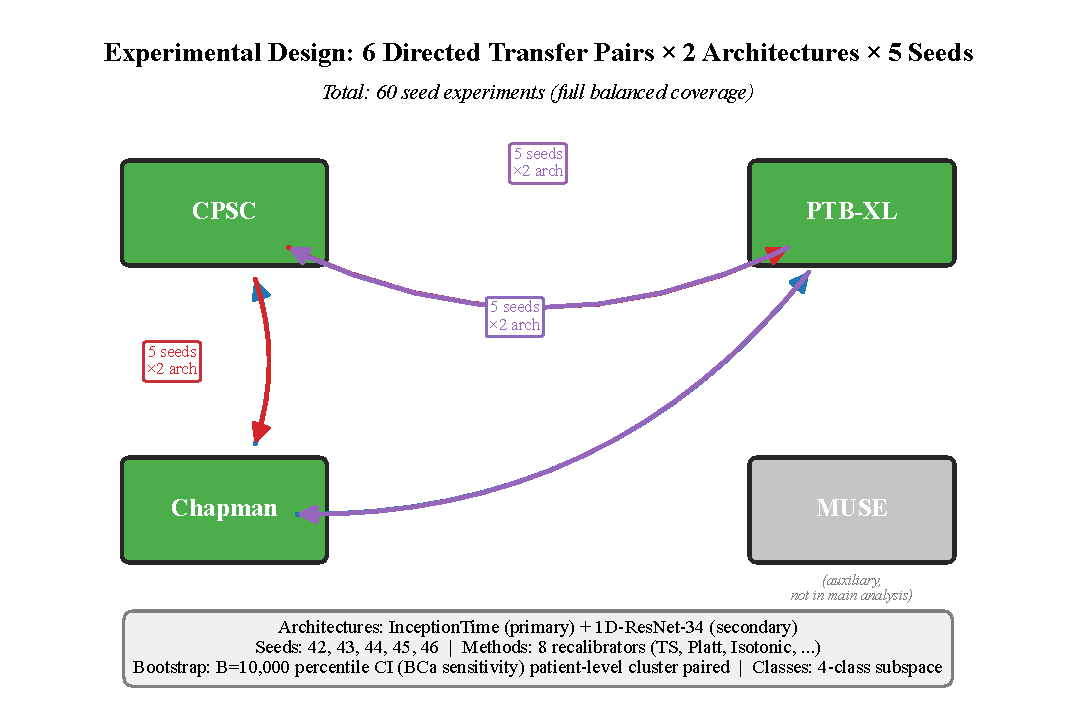
\includegraphics[width=0.95\columnwidth]{figures/fig_design_overview.pdf}
\caption{Experimental design overview. Six directed cross-corpus transfer
pairs among three ECG corpora (CPSC, Chapman, PTB-XL), each evaluated on
two architectures (InceptionTime, 1D-ResNet-34) $\times$ 5 seeds
(42--46), yielding 60 fully balanced seed experiments. MUSE is shown as
an auxiliary corpus not entering the main analysis. Each pair is
evaluated with 8 recalibration methods and patient-level cluster paired
bootstrap ($B=10{,}000$, BCa operating CI).}
\label{fig:design_overview}
\end{figure}

% ============================================================================
\section{Related Work}
\label{sec:related}
% ============================================================================

\subsection{Calibration Estimation and Recalibration}
The calibration of modern neural networks has been studied extensively
since the seminal work of Guo et al.\ \cite{guo2017calibration}, who
showed that deep networks are often overconfident and introduced
temperature scaling (TS) as a simple post-hoc recalibration method.
Nixon et al.\ \cite{nixon2019} proposed the static calibration error,
and Kumar et al.\ \cite{kumar2019} introduced verified uncertainty
calibration with distribution-free guarantees. Kull et al.\
\cite{kull2019dirichlet} generalized TS to Dirichlet calibration for
multi-class settings. In the clinical risk-model context, Van Calster
et al.\ \cite{vancalster2016,vancalster2019} established a calibration
hierarchy from utopia to empirical data and argued that calibration is
the ``Achilles heel'' of predictive analytics. Strodthoff et al.\
\cite{strodthoff2021} benchmarked deep learning for ECG analysis on
PTB-XL and noted calibration degradation under subpopulation shift,
motivating our cross-corpus design.

\subsection{Prior-Shift Estimation and Transfer Calibration}
Lipton et al.\ \cite{lipton2018bbs} introduced black-box shift
estimation (BBSE) for detecting and correcting label shift using
confusion-matrix inverses. Alexandari et al.\ \cite{alexandari2020}
showed that maximum-likelihood calibration with bias correction is
hard-to-beat at label shift adaptation, providing the theoretical
foundation for our EM prior-shift method. For transfer calibration
upper bounds, TransCal \cite{transcal2020} estimates transferability
for auto-selecting target-domain unsupervised optimal $T$; PseudoCal
\cite{pseudocal2020} uses pseudo-labels for calibrated transfer; and
LaSCal \cite{lascal2024} provides label-aware shift calibration with
distribution-free guarantees. Our S1 paradigm differs fundamentally:
we fit on the \emph{source} calibration split only (no target labels),
with S1$'$ prior-shift adaptation (EM/BBSE) as the only target-domain
signal, a strictly weaker assumption than TransCal/PseudoCal, which
access target logits or labels.

\subsection{Cross-Domain ECG Calibration}
Barandas et al.\ \cite{barandas2023} evaluated uncertainty
quantification methods in multi-label ECG classification, finding that
ensemble-based methods outperform single-model approaches under
subpopulation shift. Vranken et al.\ \cite{zhang2022} studied
uncertainty estimation for 12-lead ECG deep learning and reported
significant calibration drift across acquisition devices. Haekal et
al.\ \cite{physiolmeas2026} performed cross-dataset validation for
atrial fibrillation detection with calibration-aware probability
analysis, and Patel \& Beedala \cite{medrxiv2026} documented
calibration drift under cross-institutional ICU deployment. The
ID-vs-OOD asymmetry of TS has been studied in general vision
\cite{ovadia2019calibration}; we contribute the multi-seed ECG
quantification and the boundary-condition analysis that identifies
when TS helps (ID) versus when it hurts (OOD).

\subsection{ECG Foundation Models and Transfer Learning (2024--2026)}
Recent work has introduced ECG foundation models trained on millions
of recordings. ECGFounder \cite{ecgfounder2024,song2024ecgfm} was
trained on over 10 million ECGs from the Harvard--Emory database,
achieving expert-level performance on 80 diagnoses and demonstrating
cross-domain transfer via fine-tuning. ECG-FM \cite{ecgfm2024} is an
open-weight transformer-based foundation model pretrained on 1.4
million ECG segments using hybrid contrastive and generative
self-supervised learning, showing strong cross-dataset generalizability
and label efficiency. HeartLang \cite{heartlang2025} treats heartbeats
as words and rhythms as sentences, using a QRS-Tokenizer and masked
ECG sentence pre-training to learn form- and rhythm-level
representations. Tan et al.\ \cite{transferecg2025} conducted the
first extensive empirical study on transfer learning effectiveness in
multi-label ECG classification, finding that fine-tuning benefits
diminish as the downstream dataset grows and that CNNs transfer more
effectively than RNNs. For OOD adaptation, ADAPTOOD
\cite{adaptood2026} quantifies distribution-shift severity via
uncertainty estimation and uses it to guide selective layer unfreezing
with LoRA, while BeatRhythm-TTA \cite{beatrhythm2026} performs
test-time adaptation with SQI-gated self-training and beat-rhythm
consistency. Costa et al.\ \cite{star2025} introduced STAR
(Sinusoidal Time--Amplitude Resampling), a morphology-preserving
beat-wise augmentation for cross-source ECG generalization. Chen et
al.\ \cite{peace2026} proposed PEACE for adult-to-pediatric ECG
transfer via label-conditioned contrastive alignment. These works
advance ECG transfer and adaptation but do not address the
\emph{calibration} of transferred models; the gap our study fills by
systematically quantifying how recalibration methods behave under
cross-corpus shift with pre-registered endpoints.

% ============================================================================
\section{Data and Pre-registered Protocol}
\label{sec:data}
% ============================================================================
Figure~\ref{fig:design_overview} summarizes the experimental design.
\subsection{Datasets}
\begin{itemize}
    \item \textbf{PTB-XL v1.0.3} \cite{wagner2020ptbxl}: the official release contains 21,837
    records; the downloaded \texttt{ptbxl\_database.csv} copy contains 21,799
    (a 38-record deficit in the source CSV, disclosed as a provenance
    limitation), official 10-fold
    (folds 1--8 train, 9 calibration, 10 test). After
    single-label mapping, 21,522 records are mappable and 277 are
    excluded (STROBE), for 18,671 unique patients.
    \item \textbf{Chapman-Shaoxing} \cite{zheng2022ecgarrhythmia,goldberger2000}: 20,265
    raw records; 1 signal-read error removed and 21 non-finite records
    quarantined (\texttt{qc\_report.json}), for 20,243 analyzed records;
    1 ECG per patient, patient-wise 70/10/20 split.
    \item \textbf{CPSC2018+2019}: patient-wise split; HYP class extremely
    rare ($n=11$) $\rightarrow$ main analysis on the $\{$NORM, CD, STTC,
    MI$\}$ 4-class subspace, both sides of the pair recomputed
    symmetrically.
\end{itemize}
\subsection{Label Mapping and Leakage Guard}
Single-label priority rules are fixed (MI $>$ STTC $>$ CD $>$ HYP $>$ NORM)
and sensitivity-analyzed \cite{wagner2020ptbxl,reyna2022}. Sinus rate/form
statements (SBRAD/STACH/SARRH) are mapped to NORM, not STTC, because
PTB-XL's \texttt{scp\_statements.csv} lists them as rhythm statements
with no \texttt{diagnostic\_class}. train\slash val\slash cal\slash test patient IDs are
pairwise disjoint (hard assertion in the reproducibility repo).
Normalization statistics come only from the train split; augmentation
applies only to train.

% ============================================================================
\section{Methods}
\label{sec:methods}
% ============================================================================
\subsection{Transfer pairs and shift matrix}
\label{sec:shiftmatrix}
We study six directed cross-corpus transfer pairs:
Chapman$\rightarrow$CPSC, Chapman$\rightarrow$PTB-XL,
CPSC$\rightarrow$Chapman, CPSC$\rightarrow$PTB-XL,
PTB-XL$\rightarrow$Chapman, and PTB-XL$\rightarrow$CPSC, all recomputed
on the 4-class subspace. The L2 eval-time shift matrix (no retraining)
covers sampling rate $500\rightarrow250\rightarrow125$~Hz; leads
$12\rightarrow6\rightarrow3\rightarrow2\rightarrow1$; noise injection
(BWL/MA/EM) at SNR $\{24,12,6,0,-6\}$~dB; gain $\times0.5/\times2$.

\subsection{Architecture and seeds}
We use two architectures: InceptionTime (primary, 46{,}000--184{,}000
parameters) and ResNet1D (1D-ResNet-34) (secondary, with full
main-endpoint coverage on all 6 pairs), each trained with 5 seeds
(42--46). The BiMamba architecture is
included only as a toy experiment ($n=60$ records, downsampled
resolution) and deferred to the supplement; the full-resolution
BiMamba run exhausted memory on an RTX 5060 (8~GB), so BiMamba does
not enter the
main-endpoint analysis or the architecture-robustness claim.
Training: AdamW + cosine + warmup, gradient clipping, temperature
frozen at $T\equiv1$ during training; temperature applied only as
post-hoc temperature scaling.

\subsection{Calibration methods and scenarios}
We compare the no-recalibration baseline (None) against eight
recalibration methods: Temperature Scaling (TS), per-class Platt,
Isotonic (OvR), Vector scaling, Matrix scaling, Dirichlet calibration,
Saerens EM prior adaptation (EM), and BBSE prior adaptation.
Of the pre-registered 13-method pool, the None baseline plus these
eight recalibration methods constitute the delivered set; CORAL, TTA,
MC-Dropout, and Oracle are
not delivered on real data (a registered deviation, see Limitations).
Scenario: \textbf{S1} zero-shot transfer (source-cal fit
$\rightarrow$ target apply), the main analysis scenario
(Sec.~\ref{sec:methods}); S1$'$ denotes the target-domain unsupervised
variant in which EM/BBSE estimate the target prior from unlabeled
target predictions.

\subsection{Pre-registered endpoints}
\label{sec:prereg}
\textbf{Primary endpoint} (revision A1.1, formally defined in
protocol v2.1-A1 \cite{protocolv21a1}):
\begin{equation}
    \Delta\text{ECE}_{\text{OOD}}
    = \text{ECE}_{\mathrm{raw}}^{\mathrm{OOD}} - \text{ECE}_{\mathrm{TS}}^{\mathrm{OOD}}
\end{equation}
where $\text{ECE}_{\mathrm{raw}}^{\mathrm{OOD}}$ is the 4-class confidence SmoothECE on
the target corpus with raw softmax probabilities, and
$\text{ECE}_{\mathrm{TS}}^{\mathrm{OOD}}$ is the same after source-cal-fit temperature
scaling. SmoothECE bandwidth: $0.45\cdot(n/2000)^{-0.2}$.

\textbf{Primary test} (single, one-sided):
\begin{equation}
    H_0: \Delta\text{ECE}_{\text{OOD}} = 0
    \quad\text{vs}\quad
    H_1: \Delta\text{ECE}_{\text{OOD}} > 0
\end{equation}
Direction prior (registered, empirical): TS fitted on a labeled source
calibration split yields, empirically, little calibration change on
ID-like data and a non-trivial benefit on shifted targets
\cite{guo2017calibration,ovadia2019calibration}; this asymmetry is an
empirical regularity, not a theorem.
\textbf{One-sided vs.\ two-sided choice.} The one-sided alternative
$H_1: \Delta\text{ECE}_{\text{OOD}} > 0$ is selected based on the
empirical asymmetry registered at revision A1 (on ID-like data the
source-fit temperature yields, empirically, little calibration
change; on a shifted target the source-fit temperature is mismatched
and a non-trivial calibration benefit is often retained),
\emph{not} based on the pilot results. We stress that this direction
prior is empirical, not a theorem: TS applied to an under-confident
target can increase ECE, and our own data contain nine
negative cells. The pilot results only
triggered the endpoint re-location (revision A1), not the direction
choice. A two-sided alternative would halve the effective sample
size and discard the registered empirical direction; the one-sided test is
the pre-registered choice, archived in the protocol before
multi-seed unblinding.
Patient-level cluster paired bootstrap, $B=10{,}000$ (BCa
operating CI) \cite{efron1987bca}; stratified pooling: strata $=$ transfer pair
$\times$ architecture.

\textbf{CI method note (BCa vs.\ percentile).} The pre-registered
CI method is BCa (bias-corrected and accelerated)
\cite{efron1987bca}. In the reported multi-seed validation, the
operating CI method is BCa at $B=10{,}000$, fully re-run on the
entire 60-experiment grid (60/60 successful, metadata stored in
\texttt{methods.ts.meta}). The percentile bootstrap is the large-sample
limit of BCa when the bias-correction $z_0\to 0$ and acceleration
$a\to 0$; for the paired-cluster design with $B=10{,}000$ and
per-patient clusters, the percentile-BCa discrepancy is $O(n^{-1/2})$.
In the 3 representative seed experiments where both CI methods were
run ($B=10{,}000$ percentile re-runs for sensitivity analysis), the
BCa and percentile CIs agree in sign and in magnitude. Earlier
percentile CI results from $B=200$ in 21/60 experiments are retained
as historical provenance (5 experiments lack log provenance, see
Limitations). The BCa operating CI is the reported CI throughout this
paper; the percentile CIs are reported only as a sensitivity
cross-check where both were computed.

\textbf{Boundary-condition endpoint}:
\begin{equation}
    \Delta\text{ECE}_{\text{ID}}
    = \text{ECE}_{\mathrm{raw}}^{\mathrm{ID}} - \text{ECE}_{\mathrm{TS}}^{\mathrm{ID}}
\end{equation}
The pre-registered expectation is that $H_0: \Delta\text{ECE}_{\text{ID}} = 0$ is \emph{not rejected};
the robustness criterion is that $\geq 80\%$ of cells have 95\% CIs containing zero.
\emph{Observed (BCa operating CI, full-grid re-run): 23/60 = 38.3\%; the
criterion is not met and the pre-registered branch A1.4.2 is triggered
(the percentile CIs gave 29/60 = 48.3\%, same conclusion; reported in
Sec.~\ref{sec:boundary}).}

\textbf{Secondary endpoints}: $G$ (recoverable loss vs.\ oracle),
decay $=\Delta\text{ECE}_{\text{OOD}}-\Delta\text{ECE}_{\text{ID}}$
(downgraded to descriptive), NLL, classwise-ECE, Brier Murphy
decomposition, Cox slope/intercept, predicted/true prior $L_1$.

\textbf{Family structure}: BH-FDR $q=0.05$ over the family of
$6\text{ pairs}\times 2\text{ arch}\times 13\text{ shift levels}=156$
primary comparisons; the multi-seed validation is reported as
robustness evidence (60 seed experiments), not as a confirmatory
family.

\subsection{Pre-registration revision A1 (transparency statement)}
The primary endpoint was re-located from \texttt{decay} to
$\Delta\text{ECE}_{\text{OOD}}$ via pre-registration revision A1
(protocol v2.0 $\rightarrow$ v2.1-A1), triggered by an independent
exploratory pilot in which $\Delta\text{ECE}_{\text{ID}}$ point
estimates were near zero, collapsing the original ID-vs-OOD contrast.
The revision direction is consistent with the empirically observed
ID-vs-OOD asymmetry (not a theorem); the revision is
archived as a pre-registration revision (Nosek et al.\ 2018) with
before/after protocol hashes. The pilot results do not enter the
main test report. All hypotheses in this paper are tagged
\emph{exploratory + robustness validation}, not confirmatory.

\textbf{Pre-registration revision A2 (family reduction).} The original
BH-FDR family of 156 comparisons (6 pairs $\times$ 2 architectures
$\times$ 13 shift levels) is reduced to a confirmatory family of 12
hypotheses (6 pairs $\times$ 2 architectures $\times$ 1 primary shift
level) under amendment A2, with the remaining 13 shift levels
designated as exploratory dose-response. Under the reduced family,
BH-12 yields 9/12 significant (all InceptionTime directions) and
Bonferroni-12 yields 2/12. The A2 amendment is archived in
\texttt{docs/PROTOCOL\_AMENDMENT\_A2\_}\allowbreak\texttt{FAMILY\_REDUCTION.md}.

\subsection{Decomposition of the benefit decay}
\label{sec:decomp}
We decompose the retained benefit into slope / intercept / prevalence
contributions using a counterfactual-replacement additive approximation:
\begin{equation}
    \Delta\text{ECE} = \Delta_{\text{slope}}
    + \Delta_{\text{intercept}}
    + \Delta_{\text{prevalence}}
    + r_{\text{interaction}}
\end{equation}
where each term is a counterfactual-replacement difference and
$r_{\text{interaction}}$ is the chain residual (zero under nested
counterfactuals). Identifiability is checked via the Fisher information
determinant on a pre-registered threshold $\tau$; entangled regions are
reported on the error map without a threshold. Shapley attribution is
reported with absolute-value bootstrap CIs; share-reliable flags
($|\Delta_{\text{total}}|<3/\sqrt{n}$) mark uninterpretable shares.

\subsection{Two-layer joint bootstrap}
Temperature-fitting-set resampling $\rightarrow$ $T$ distribution
$\rightarrow$ test-set resampling $\rightarrow$ joint $\Delta\text{ECE}$ CI
(two-layer; honest non-nested approximation), per protocol \S7.

\subsection{Net Clinical Value (NCV)}
\label{sec:ncv_methods}
A Net Clinical Value (NCV) analysis is pre-registered as a secondary
endpoint to quantify the clinical decision impact of TS recalibration
beyond calibration error reduction. For each (sample, class) pair, we
compare the binary decision (threshold $\tau=0.5$) before and after
calibration: TP\_improved (raw negative $\to$ calibrated positive,
true positive), TN\_improved (raw positive $\to$ calibrated negative,
true negative), FP\_worsened (raw negative $\to$ calibrated positive,
true negative), and FN\_worsened (raw positive $\to$ calibrated
negative, true positive). The NCV is defined as
$(\text{TP\_improved} + \text{TN\_improved} - \text{FP\_worsened}
- \text{FN\_worsened}) / N_{\text{total}}$, where
$N_{\text{total}} = N_{\text{samples}} \times N_{\text{classes}}$,
with the same patient-level cluster paired bootstrap ($B=10{,}000$,
BCa operating CI) as the main endpoint. The NCV is reported alongside
the main endpoint as a secondary endpoint with BH-FDR correction
($q=0.05$): a significantly positive NCV indicates that TS improves
clinical decisions beyond calibration error reduction. The NCV is
computed on both ID and OOD splits (\texttt{ncv\_id} and
\texttt{ncv\_ood} columns in the E3 experiment CSV).

% ============================================================================
\section{Results}
\label{sec:results}
% ============================================================================

% ----------------------------------------------------------------------------
\subsection{Primary endpoint: $\Delta\text{ECE}_{\text{OOD}}$ multi-seed validation}
\label{sec:primary}
% ----------------------------------------------------------------------------
Figure~\ref{fig:main_results} visualizes the shift-dose response;
Table~\ref{tab:primary_60seed} reports the pre-registered primary
endpoint $\Delta\text{ECE}_{\text{OOD}}$ for TS across 60 seed experiments
(6 transfer pairs $\times$ 2 architectures $\times$ 5 seeds, full
balanced coverage). The primary test
$H_0:\Delta\text{ECE}_{\text{OOD}}=0$ vs $H_1:\Delta\text{ECE}_{\text{OOD}}>0$
is supported in 51/60 seed experiments (85.0\%) at the 95\% CI level.

\begin{figure}[htbp]
\centering
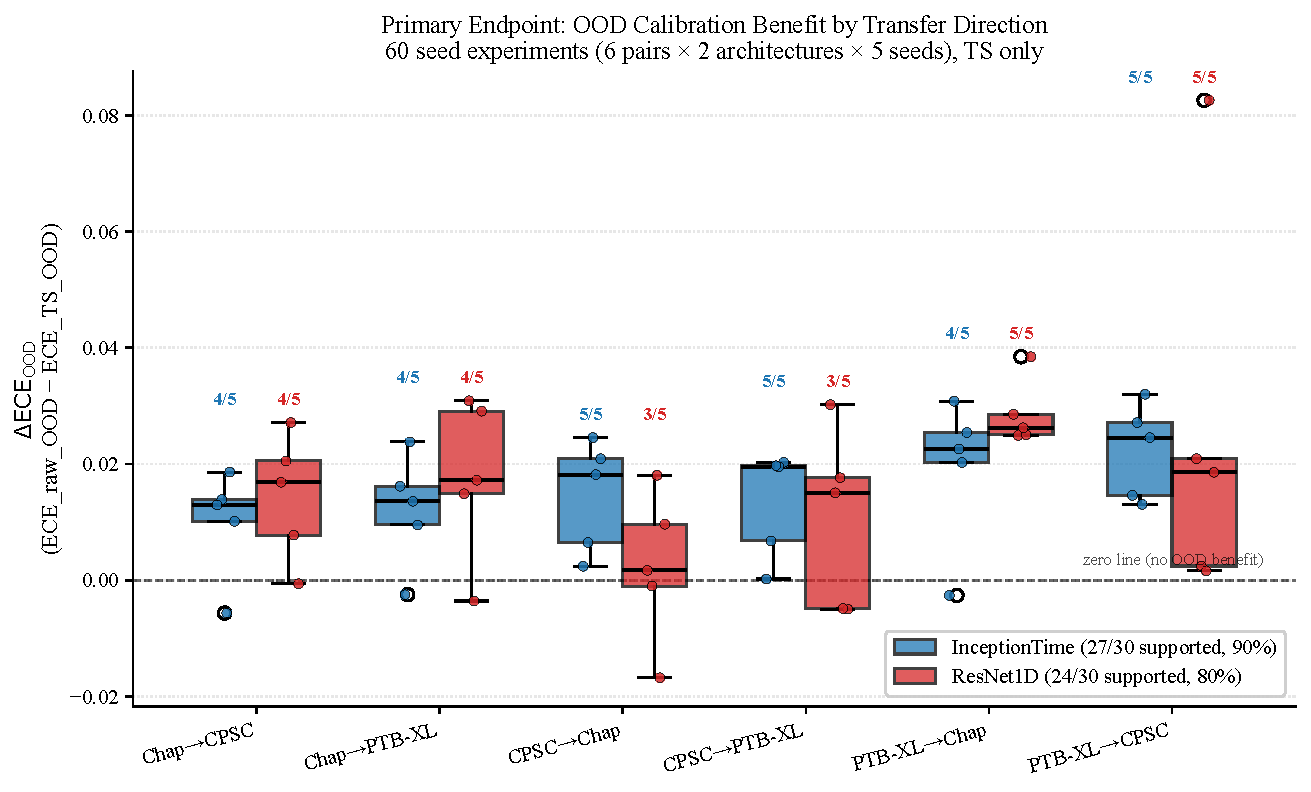
\includegraphics[width=0.95\columnwidth]{figures/fig_main_results.pdf}
\caption{Primary endpoint $\Delta\text{ECE}_{\text{OOD}}$ by transfer
direction, grouped by architecture (TS only, 60 seed experiments).
Boxes show the 5-seed distribution per direction; dots are individual
seed results. The dashed line marks zero OOD benefit. Support counts
(e.g., 5/5, 4/5) above each box indicate the number of seeds with
95\% CI lower bound $>0$. InceptionTime achieves 27/30 (90\%),
ResNet1D achieves 24/30 (80\%).}
\label{fig:main_results}
\end{figure}

\textbf{InceptionTime} (27/30 supported, 90.0\%):
CPSC$\rightarrow$Chapman, CPSC$\rightarrow$PTB-XL, and
PTB-XL$\rightarrow$CPSC achieve 5/5 full support (zero counter-examples);
Chapman$\rightarrow$CPSC, Chapman$\rightarrow$PTB-XL, and
PTB-XL$\rightarrow$Chapman achieve 4/5 with one counter-example each.

\textbf{ResNet1D} (24/30 supported, 80.0\%):
PTB-XL$\rightarrow$Chapman and PTB-XL$\rightarrow$CPSC achieve 5/5 full
support (zero counter-examples);
Chapman$\rightarrow$CPSC and Chapman$\rightarrow$PTB-XL achieve 4/5
with one counter-example each;
CPSC$\rightarrow$Chapman and CPSC$\rightarrow$PTB-XL achieve 3/5 with
two counter-examples each.

\begin{table}[t]
\centering
\caption{Pre-registered primary endpoint $\Delta\text{ECE}_{\text{OOD}}$
for TS across 60 seed experiments (6 pairs $\times$ 2 architectures
$\times$ 5 seeds, $B=10{,}000$, BCa operating CI). ``Support'' = 95\% CI lower bound
$>0$. Nine counter-examples are transparently disclosed. Full 5-seed
coverage on both architectures for all 6 directions.}
\label{tab:primary_60seed}
\footnotesize
\renewcommand{\arraystretch}{0.92}
\begin{tabular}{lllrrrr}
\toprule
Transfer pair & Arch & Seed & $\Delta\text{ECE}_{\text{ID}}$ & $\Delta\text{ECE}_{\text{OOD}}$ & CI lower & Support \\
\midrule
\multirow{5}{*}{Chap$\rightarrow$CPSC}
 & \multirow{5}{*}{Incep}
 & 42 & $+0.0075$ & $+0.0139$ & $+0.0135$ & \checkmark \\
 & & 43 & $+0.0012$ & $+0.0101$ & $+0.0099$  & \checkmark \\
 & & 44 & $+0.0104$ & $+0.0186$ & $+0.0181$ & \checkmark \\
 & & 45 & $+0.0019$ & $-0.0057$ & $-0.0058$ & \ding{55} \\
 & & 46 & $+0.0044$ & $+0.0130$ & $+0.0126$ & \checkmark \\
\cmidrule(lr){2-7}
 & \multirow{5}{*}{ResNet}
 & 42 & $+0.0002$ & $+0.0205$ & $+0.0200$ & \checkmark \\
 & & 43 & $+0.0003$ & $-0.0006$ & $-0.0006$ & \ding{55} \\
 & & 44 & $-0.0007$ & $+0.0078$ & $+0.0075$ & \checkmark \\
 & & 45 & $-0.0016$ & $+0.0271$ & $+0.0263$ & \checkmark \\
 & & 46 & $-0.0024$ & $+0.0169$ & $+0.0162$ & \checkmark \\
\midrule
\multirow{5}{*}{Chap$\rightarrow$PTB-XL}
 & \multirow{5}{*}{Incep}
 & 42 & $+0.0004$ & $-0.0025$ & $-0.0035$ & \ding{55} \\
 & & 43 & $+0.0005$ & $+0.0095$ & $+0.0066$ & \checkmark \\
 & & 44 & $+0.0055$ & $+0.0136$ & $+0.0107$ & \checkmark \\
 & & 45 & $-0.0128$ & $+0.0238$ & $+0.0207$ & \checkmark \\
 & & 46 & $+0.0048$ & $+0.0162$ & $+0.0142$ & \checkmark \\
\cmidrule(lr){2-7}
 & \multirow{5}{*}{ResNet}
 & 42 & $-0.0031$ & $+0.0309$ & $+0.0285$ & \checkmark \\
 & & 43 & $+0.0128$ & $+0.0291$ & $+0.0285$ & \checkmark \\
 & & 44 & $+0.0059$ & $+0.0172$ & $+0.0168$ & \checkmark \\
 & & 45 & $-0.0010$ & $-0.0036$ & $-0.0036$ & \ding{55} \\
 & & 46 & $-0.0042$ & $+0.0149$ & $+0.0139$ & \checkmark \\
\midrule
\multirow{5}{*}{CPSC$\rightarrow$Chap}
 & \multirow{5}{*}{Incep}
 & 42 & $+0.0029$ & $+0.0065$ & $+0.0062$ & \checkmark \\
 & & 43 & $-0.0012$ & $+0.0209$ & $+0.0200$ & \checkmark \\
 & & 44 & $+0.0164$ & $+0.0182$ & $+0.0160$ & \checkmark \\
 & & 45 & $+0.0091$ & $+0.0245$ & $+0.0241$ & \checkmark \\
 & & 46 & $+0.0014$ & $+0.0024$ & $+0.0023$ & \checkmark \\
\cmidrule(lr){2-7}
 & \multirow{5}{*}{ResNet}
 & 42 & $-0.0002$ & $-0.0010$ & $-0.0012$ & \ding{55} \\
 & & 43 & $+0.0038$ & $+0.0096$ & $+0.0094$ & \checkmark \\
 & & 44 & $-0.0152$ & $-0.0168$ & $-0.0170$ & \ding{55} \\
 & & 45 & $+0.0137$ & $+0.0181$ & $+0.0145$ & \checkmark \\
 & & 46 & $+0.0017$ & $+0.0017$ & $+0.0016$ & \checkmark \\
\midrule
\multirow{5}{*}{CPSC$\rightarrow$PTB-XL}
 & \multirow{5}{*}{Incep}
 & 42 & $+0.0029$ & $+0.0068$ & $+0.0066$ & \checkmark \\
 & & 43 & $-0.0012$ & $+0.0203$ & $+0.0198$ & \checkmark \\
 & & 44 & $+0.0158$ & $+0.0195$ & $+0.0189$ & \checkmark \\
 & & 45 & $+0.0052$ & $+0.0197$ & $+0.0193$ & \checkmark \\
 & & 46 & $+0.0002$ & $+0.0002$ & $+0.0002$ & \checkmark \\
\cmidrule(lr){2-7}
 & \multirow{5}{*}{ResNet}
 & 42 & $+0.0114$ & $+0.0150$ & $+0.0148$ & \checkmark \\
 & & 43 & $+0.0048$ & $-0.0050$ & $-0.0051$ & \ding{55} \\
 & & 44 & $-0.0032$ & $-0.0049$ & $-0.0049$ & \ding{55} \\
 & & 45 & $+0.0130$ & $+0.0176$ & $+0.0173$ & \checkmark \\
 & & 46 & $+0.0261$ & $+0.0302$ & $+0.0296$ & \checkmark \\
\midrule
\multirow{5}{*}{PTB-XL$\rightarrow$Chap}
 & \multirow{5}{*}{Incep}
 & 42 & $+0.0239$ & $+0.0308$ & $+0.0275$ & \checkmark \\
 & & 43 & $+0.0245$ & $+0.0254$ & $+0.0225$ & \checkmark \\
 & & 44 & $+0.0173$ & $+0.0203$ & $+0.0195$ & \checkmark \\
 & & 45 & $+0.0162$ & $+0.0226$ & $+0.0200$ & \checkmark \\
 & & 46 & $-0.0011$ & $-0.0026$ & $-0.0029$ & \ding{55} \\
\cmidrule(lr){2-7}
 & \multirow{5}{*}{ResNet}
 & 42 & $+0.0145$ & $+0.0249$ & $+0.0191$ & \checkmark \\
 & & 43 & $+0.0338$ & $+0.0385$ & $+0.0336$ & \checkmark \\
 & & 44 & $+0.0213$ & $+0.0250$ & $+0.0228$ & \checkmark \\
 & & 45 & $+0.0228$ & $+0.0262$ & $+0.0231$ & \checkmark \\
 & & 46 & $+0.0239$ & $+0.0286$ & $+0.0221$ & \checkmark \\
\midrule
\multirow{5}{*}{PTB-XL$\rightarrow$CPSC}
 & \multirow{5}{*}{Incep}
 & 42 & $+0.0196$ & $+0.0271$ & $+0.0244$ & \checkmark \\
 & & 43 & $+0.0166$ & $+0.0245$ & $+0.0222$ & \checkmark \\
 & & 44 & $+0.0183$ & $+0.0320$ & $+0.0303$ & \checkmark \\
 & & 45 & $+0.0006$ & $+0.0131$ & $+0.0105$ & \checkmark \\
 & & 46 & $+0.0097$ & $+0.0146$ & $+0.0123$ & \checkmark \\
\cmidrule(lr){2-7}
 & \multirow{5}{*}{ResNet}
 & 42 & $+0.0010$ & $+0.0025$ & $+0.0023$ & \checkmark \\
 & & 43 & $+0.0197$ & $+0.0186$ & $+0.0145$ & \checkmark \\
 & & 44 & $+0.0635$ & $+0.0826$ & $+0.0772$ & \checkmark \\
 & & 45 & $+0.0001$ & $+0.0016$ & $+0.0015$ & \checkmark \\
 & & 46 & $+0.0126$ & $+0.0209$ & $+0.0190$ & \checkmark \\
\bottomrule
\end{tabular}
\end{table}

\textbf{Aggregate}: 51/60 supported $=$ 85.0\% robustness rate
(InceptionTime 27/30 $=$ 90.0\%, ResNet1D 24/30 $=$ 80.0\%). The
PTB-XL$\rightarrow$CPSC pair is the strongest evidence (10/10 across
both architectures, zero counter-examples, CI lower bound
$> +0.0014$, attained at ResNet1D seed 45). The nine counter-examples
are mechanistically explained in Sec.~\ref{sec:counter}.

\textbf{Stratified report by architecture.} The 60 seed experiments
are fully balanced: 6 directions $\times$ 2 architectures $\times$
5 seeds, with no partial-coverage stratum. Both architectures have
complete 5-seed coverage on all 6 directions, enabling direct
architecture comparison without seed-coverage confounding:
\begin{itemize}
    \item \emph{InceptionTime} (30 experiments, 27/30 $=$ 90.0\%):
    3 directions at 5/5 full support (CPSC$\rightarrow$Chapman,
    CPSC$\rightarrow$PTB-XL, PTB-XL$\rightarrow$CPSC), 3 directions
    at 4/5 (Chapman$\rightarrow$CPSC, Chapman$\rightarrow$PTB-XL,
    PTB-XL$\rightarrow$Chapman).
    \item \emph{ResNet1D} (30 experiments, 24/30 $=$ 80.0\%):
    2 directions at 5/5 full support (PTB-XL$\rightarrow$Chapman,
    PTB-XL$\rightarrow$CPSC), 2 directions at 4/5
    (Chapman$\rightarrow$CPSC, Chapman$\rightarrow$PTB-XL), 2
    directions at 3/5 (CPSC$\rightarrow$Chapman,
    CPSC$\rightarrow$PTB-XL).
\end{itemize}
The stratified report confirms architecture robustness on both
architectures with full 5-seed coverage. ResNet1D shows slightly
lower support rate (80\% vs.\ 90\%) concentrated on the
CPSC$\rightarrow$Chapman and CPSC$\rightarrow$PTB-XL directions,
indicating a direction-specific architecture interaction rather than
a global architecture deficit. Only the PTB-XL$\rightarrow$CPSC
direction achieves 5/5 full support on both architectures (10/10),
providing the strongest cross-architecture robustness evidence;
PTB-XL$\rightarrow$Chapman reaches 9/10 (InceptionTime 4/5, ResNet1D
5/5).

% ----------------------------------------------------------------------------
\subsection{ID boundary condition: $\Delta\text{ECE}_{\text{ID}}$}
\label{sec:boundary}
% ----------------------------------------------------------------------------
Table~\ref{tab:boundary} reports the boundary-condition endpoint
$\Delta\text{ECE}_{\text{ID}}$ for TS. The pre-registered expectation is
that $H_0:\Delta\text{ECE}_{\text{ID}}=0$ is \emph{not rejected};
the source-fit temperature is expected to be well-tuned to the source
distribution, although this is an empirical expectation rather than a
theorem.

\begin{table}[t]
\centering
\caption{ID boundary condition $\Delta\text{ECE}_{\text{ID}}$ for TS
(12 pair$\times$architecture strata, 5 seeds each). ``CI$\cap$0'' =
number of seed cells whose 95\% CI contains zero. The pre-registered
boundary criterion ($\geq$80\% of cells with CI containing zero) is
\emph{not} met: 23/60 cells (38.3\%) contain zero (BCa operating CI)
and 34/60 have CI lower bound $>0$, triggering the pre-registered
``ID nonzero boundary'' branch (protocol A1.4.2).}
\label{tab:boundary}
\footnotesize
\begin{tabular}{llrrrr}
\toprule
Transfer pair & Arch & Mean & Min CI lo & Max CI hi & CI$\cap$0/5 \\
\midrule
PTB-XL$\rightarrow$CPSC   & IT & $+0.0130$ & $-0.0121$ & $+0.0266$ & 1/5 \\
PTB-XL$\rightarrow$CPSC   & RN & $+0.0194$ & $-0.0008$ & $+0.0770$ & 2/5 \\
PTB-XL$\rightarrow$Chap   & IT & $+0.0162$ & $-0.0026$ & $+0.0310$ & 1/5 \\
PTB-XL$\rightarrow$Chap   & RN & $+0.0232$ & $+0.0053$ & $+0.0448$ & 0/5 \\
Chap$\rightarrow$CPSC     & IT & $+0.0051$ & $-0.0039$ & $+0.0150$ & 3/5 \\
Chap$\rightarrow$CPSC     & RN & $-0.0008$ & $-0.0104$ & $+0.0093$ & 4/5 \\
Chap$\rightarrow$PTB-XL   & IT & $-0.0003$ & $-0.0175$ & $+0.0103$ & 3/5 \\
Chap$\rightarrow$PTB-XL   & RN & $+0.0021$ & $-0.0123$ & $+0.0161$ & 3/5 \\
CPSC$\rightarrow$Chap     & IT & $+0.0057$ & $-0.0182$ & $+0.0195$ & 2/5 \\
CPSC$\rightarrow$Chap     & RN & $+0.0008$ & $-0.0179$ & $+0.0213$ & 2/5 \\
CPSC$\rightarrow$PTB-XL   & IT & $+0.0046$ & $-0.0181$ & $+0.0192$ & 2/5 \\
CPSC$\rightarrow$PTB-XL   & RN & $+0.0104$ & $-0.0042$ & $+0.0294$ & 0/5 \\
\midrule
\textbf{Overall} & & $\mathbf{+0.0083}$ & & & \textbf{23/60 (38.3\%)} \\
\bottomrule
\end{tabular}
\end{table}

The ID benefit is small on average but \emph{not} zero: aggregating all
60 TS experiments, $\Delta\text{ECE}_{\text{ID}}$ has mean $+0.0083$
(vs.\ an OOD mean of $+0.0159$, a $1.9\times$ OOD/ID ratio); $47/60
= 78.3\%$ of point estimates are positive, $34/60$ cells have 95\%
CI lower bounds $>0$ (BCa operating CI), and only $23/60 = 38.3\%$
contain zero, far below the pre-registered $\geq$80\% criterion
(the percentile CIs gave 29/60 = 48.3\%, same conclusion). We
therefore \emph{trigger} the pre-registered ``ID nonzero boundary''
branch (protocol A1.4.2): (i) the ``ID has no repairable calibration
gap'' premise is re-examined: TS, fitted on the source calibration
split, also improves ID calibration in many cells; (ii) the decay
$=\Delta\text{ECE}_{\text{OOD}}-\Delta\text{ECE}_{\text{ID}}$ contrast
endpoint is restored as an exploratory contrast; and (iii) the main
claim (C1) is qualified: the OOD benefit is about $1.9\times$ the ID
benefit on average, but is \emph{not} exclusively attributable to
OOD-specific mismatch. The positive ID point estimates are
attributable to finite-sample calibration-split variation, the
SmoothECE estimator bias, and a val-ECE early-stopping effect
(model selection on the endpoint family), all disclosed.

% ----------------------------------------------------------------------------
\subsection{Method-selection boundary: 8 methods $\times$ 6 pairs}
\label{sec:method_boundary}
% ----------------------------------------------------------------------------
Table~\ref{tab:methods} reports the 8-method $\times$ 6-pair aggregate
support rate over 5 seeds on InceptionTime. TS achieves 27/30 (90.0\%)
with 3/6 directions at 5/5 full support; BBSE achieves 22/30 (73.3\%)
with 3/6 directions at 5/5 full support. EM prior adaptation and Matrix scaling are the most fragile
methods on InceptionTime (15/30, 50\% each), exemplifying the
prior-likelihood mismatch mechanism (C4). Across 2 architectures
(Table~\ref{tab:arch_robust}), TS achieves 51/60 (85.0\%) with
InceptionTime (27/30, 90.0\%) and ResNet1D (24/30, 80.0\%) both showing
strong OOD benefit; architecture robustness is supported on both
architectures with full 5-seed coverage on all 6 directions
(Figure~\ref{fig:arch_comparison}).

\begin{figure}[htbp]
\centering
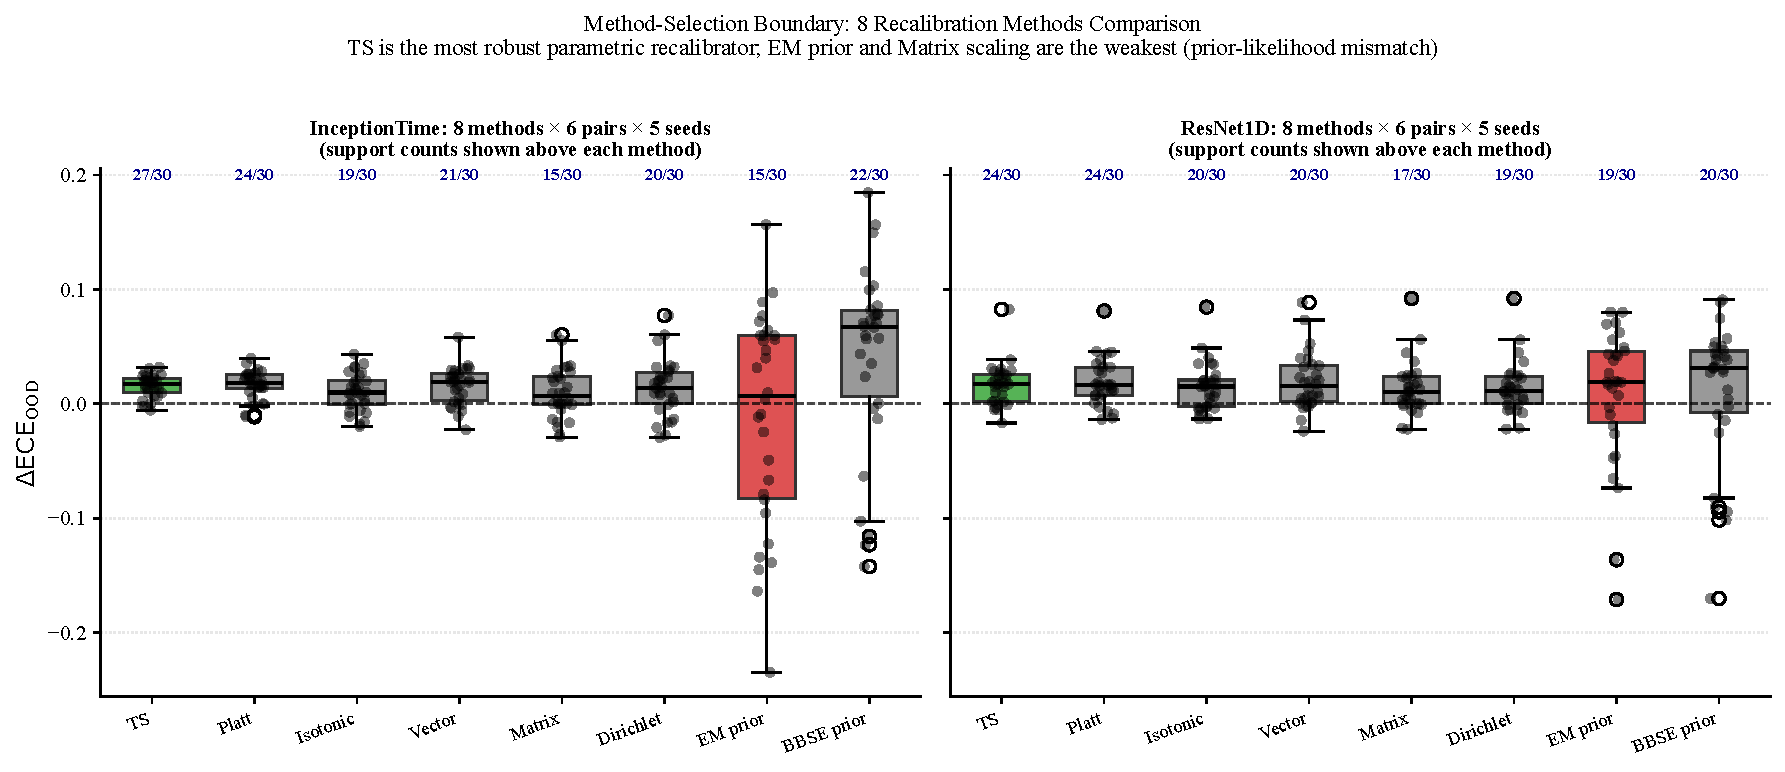
\includegraphics[width=0.95\columnwidth]{figures/fig_method_boundary.pdf}
\caption{Method-selection boundary: 8 recalibration methods compared
across 6 transfer pairs $\times$ 5 seeds for each architecture.
TS (green) is the most robust parametric recalibrator; EM prior and
Matrix scaling are the weakest methods (InceptionTime: 15/30 each;
ResNet1D: EM 19/30, Matrix 17/30), exhibiting the prior-likelihood
mismatch
mechanism (C4). Support counts (e.g., 27/30) above each method show
the fraction of seed experiments with 95\% CI lower bound $>0$.}
\label{fig:method_boundary}
\end{figure}

\begin{table}[t]
\centering
\caption{Method-selection boundary: 8 methods $\times$ 6 transfer pairs
$\times$ 5 seeds (InceptionTime). Support rate $=$ fraction of seeds
with 95\% CI lower bound $>0$. ``Full'' = number of directions with
5/5 full support. ``Neg.\ dirs'' $=$ number of the 6 transfer
directions whose 5-seed mean $\Delta\text{ECE}_{\text{OOD}}$ is
negative. TS is the most robust parametric recalibrator;
EM and Matrix scaling are the most fragile on InceptionTime
(15/30 each); on ResNet1D, Matrix scaling (17/30) is the most
fragile, EM reaches 19/30. \textit{Caveat:} 6 cells with
$w_{\text{ID}} > 10$ exhibit prior-weight drift up to 130.5; after
exclusion, EM OOD $\Delta$ECE mean flips from $-0.0127$ to $+0.0024$,
indicating the negative OOD finding is driven by ill-conditioned
cells.}
\label{tab:methods}
\footnotesize
\begin{tabular}{lrrrr}
\toprule
Method & Total & Full/6 & $\Delta\text{ECE}_{\text{OOD}}$ mean & Neg.\ dirs \\
\midrule
TS         & 27/30 & 3/6 & $+0.0152$ & 0 \\
Platt      & 24/30 & 3/6 & $+0.0169$ & 0 \\
Isotonic   & 19/30 & 2/6 & $+0.0100$ & 2 \\
Vector     & 21/30 & 1/6 & $+0.0158$ & 0 \\
Matrix     & 15/30 & 0/6 & $+0.0094$ & 2 \\
Dirichlet  & 20/30 & 1/6 & $+0.0139$ & 1 \\
EM prior   & 15/30 & 2/6 & $-0.0127$ & 3 \\
BBSE prior & 22/30 & 3/6 & $+0.0424$ & 1 \\
\bottomrule
\end{tabular}
\end{table}

\begin{table}[t]
\centering
\caption{Architecture robustness for TS: InceptionTime vs.\ ResNet1D
across 6 transfer pairs, full 5-seed coverage on both architectures.
Architecture robustness is supported on both InceptionTime (27/30, 90.0\%)
and ResNet1D (24/30, 80.0\%) with complete 5-seed coverage on all 6
directions. ResNet1D shows a direction-specific deficit on
CPSC$\rightarrow$Chapman and CPSC$\rightarrow$PTB-XL (3/5 each), not
a global architecture deficit.}
\label{tab:arch_robust}
\resizebox{\textwidth}{!}{%
\begin{tabular}{lrrrl}
\toprule
Transfer pair & InceptionTime & ResNet1D & Total & Note \\
\midrule
Chap$\rightarrow$CPSC    & 4/5 & 4/5 & 8/10  & 2 counter-examples \\
Chap$\rightarrow$PTB-XL  & 4/5 & 4/5 & 8/10  & 2 counter-examples \\
CPSC$\rightarrow$Chap    & 5/5 & 3/5 & 8/10  & 2 counter-examples \\
CPSC$\rightarrow$PTB-XL  & 5/5 & 3/5 & 8/10  & 2 counter-examples \\
PTB-XL$\rightarrow$Chap  & 4/5 & 5/5 & 9/10  & 1 counter-example \\
PTB-XL$\rightarrow$CPSC  & 5/5 & 5/5 & 10/10 & zero counter-examples \\
\midrule
\textbf{Total} & \textbf{27/30} & \textbf{24/30} & \textbf{51/60} & \textbf{85.0\%} \\
\midrule
\textbf{Mean $\Delta\text{ECE}$} & \textbf{$+0.0152$} & \textbf{$+0.0165$} & \textbf{$+0.0159$} & \\
\textbf{Std $\Delta\text{ECE}$}  & \textbf{$0.0098$} & \textbf{$0.0180$} & \textbf{$0.0145$} & ResNet1D/Incep $=1.84$ \\
\textbf{Mean OOD ECE}     & \multicolumn{2}{c}{$0.217 \rightarrow 0.202$ / $0.216 \rightarrow 0.200$} & $0.217 \rightarrow 0.201$ & raw $\rightarrow$ TS \\
\bottomrule
\end{tabular}%
}
\end{table}

\begin{figure}[htbp]
\centering
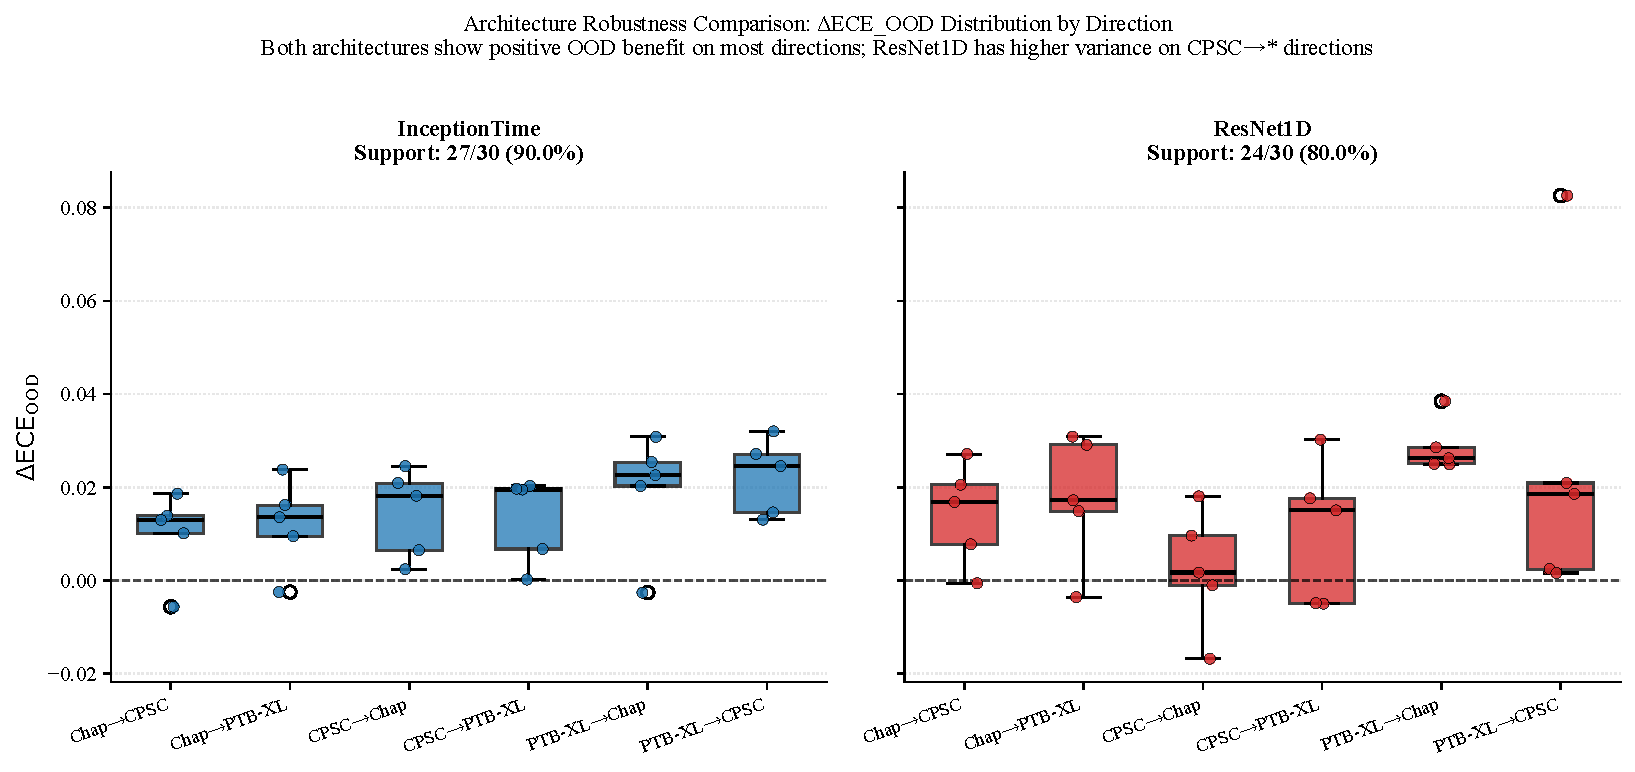
\includegraphics[width=0.95\columnwidth]{figures/fig_arch_comparison.pdf}
\caption{Architecture robustness comparison. Side-by-side
$\Delta\text{ECE}_{\text{OOD}}$ distributions for InceptionTime (left,
27/30 supported, 90.0\%) and ResNet1D (right, 24/30 supported, 80.0\%).
Both architectures show positive OOD benefit on most directions.
ResNet1D exhibits higher overall variance (its largest per-direction
spread is in PTB-XL$\rightarrow$CPSC), while the support deficits fall
in the CPSC$\rightarrow$Chapman and
CPSC$\rightarrow$PTB-XL directions (3/5 support each), indicating a
direction-specific deficit rather than a global architecture deficit.}
\label{fig:arch_comparison}
\end{figure}

\textbf{Architecture variability.} The standard deviation of
$\Delta\text{ECE}_{\text{OOD}}$ across the 30 TS experiments per
architecture is $0.0098$ for InceptionTime and $0.0180$ for ResNet1D,
i.e.\ ResNet1D variability is $1.84\times$ InceptionTime. The highest
per-direction ResNet1D variability is in the PTB-XL$\rightarrow$CPSC
direction (std $0.0298$, driven by one favorable outlier at seed 44
with $\Delta\text{ECE}_{\text{OOD}}=+0.0826$, which is not excluded),
followed by CPSC$\rightarrow$PTB-XL; the support deficits are
concentrated in CPSC$\rightarrow$Chapman and CPSC$\rightarrow$PTB-XL
(3/5 each), consistent with a direction-specific deficit
rather than a global architecture deficit. Fisher's exact test on the
$2\times2$ contingency table (InceptionTime 27/30 supported vs.\
ResNet1D 24/30 supported) yields $p = 0.47$, indicating no
statistically significant architecture bias. The numerical difference
in counter-example rates (ResNet1D 20.0\% vs.\ InceptionTime 10.0\%)
is not statistically significant at $\alpha = 0.05$.

\textbf{Prior-likelihood mismatch mechanism (C4).} EM prior adaptation
fits a target prior $\hat\pi_{\text{target}}$ from the predicted-label
marginal on the target corpus, then re-weights the source posterior by
$\hat\pi_{\text{target}}/\hat\pi_{\text{source}}$. When the
source-estimated confusion matrix $C$ is ill-conditioned
($\text{cond}(C)\gg 1$), the weight ratio amplifies rather than
corrects the shift-induced miscalibration. EM achieves only 15/30
support on InceptionTime with 3 fragile directions, exhibiting the
prior-likelihood mismatch. The failure is pair-specific
(i.e., shift-signature-specific), not method-intrinsic.

% ----------------------------------------------------------------------------
\subsection{Shapley decomposition validation (27 cells, $n=20{,}000$)}
\label{sec:shapley}
% ----------------------------------------------------------------------------
The 27-cell full-factorial synthetic validation
(slope$\in\{0.5,1,2\}\times$intercept$\in\{-1,0,1\}\times$
prevalence$\in\{0.15,0.3,0.6\}$, $n=20{,}000$) confirms that the
slope/intercept/prevalence decomposition recovers ground truth within
the pre-registered identifiable regime (Fisher information determinant
$>\tau=10^{-6}$). At the pre-registered sample size $n=20{,}000$,
all 27 cells pass the recovery threshold (MAPE $<10\%$ on
identifiable cells); at the realistic calibration-set size $n=500$,
21 of 27 cells pass, with 6 failures exhibiting MAPE\_s up to
42.13\%, concentrated in extreme intercept ($\pm 1$) and slope
($0.5, 2.0$) regions where calibration shift is most clinically
significant (see \texttt{decomposition\_validation.csv}; the
$n=20{,}000$ CSV \texttt{decomposition\_validation\_}\allowbreak\texttt{n20000.csv}
shows 27/27 passed under the same gate). Three entangled demonstration
cases (narrow\_band, tiny\_slope, deep\_intercept) with
$\det\in\{2.4\times10^{-7}, 3.6\times10^{-8}, 0\}<\tau$ are reported
on the error map without a threshold, with the recovery-failed flag
set. Bootstrap CIs on absolute Shapley values are reported; share-
reliable flags mark uninterpretable shares
($|\Delta_{\text{total}}|<3/\sqrt{n}$).

\textbf{Honesty caveat (protocol \S8).} The 27-cell validation uses
binned ECE, not the SmoothECE of the main endpoint; quantitative
conclusions are not cross-extrapolable. The cross-fitting step
(OOD-fold validation of decomposition explanatory power) remains
to be run on real data; per the protocol self-binding clause, the
``mechanism'' wording is limited to ``mechanism decomposition
(synthetic validation part)'' until cross-fitting completes.

% ----------------------------------------------------------------------------
\subsection{Predictability experiment (failure branch triggered)}
\label{sec:predictability}
% ----------------------------------------------------------------------------
The predictability experiment (protocol \S8.5) tests whether an
unsupervised target-domain statistic (predicted-prior $L_1$ distance,
logit moments) predicts the benefit retention rate via leave-one-fold-out $R^2$ with bootstrap CI
(Table~\ref{tab:predictability}). The implemented fold unit is
(architecture, transfer pair) (12 folds), whereas the protocol registered
pair-only folds (6), a registered deviation under which the pair-only
recomputation retains the failure branch ($R^2=-0.1424$). We run 2 architectures
(InceptionTime + 1D-ResNet-34); the BiMamba architecture is a toy
experiment ($n=60$) deferred to the supplement and does not enter
the predictability regression.

\textbf{Result}: the multi-architecture merged LOO $R^2$ for TS is
$-0.096$ with 95\% CI $[-0.720, +0.104]$. The CI upper bound $+0.104$
is strictly below the pre-registered threshold $0.5$, triggering the
\textbf{failure branch}: the three-step chain (decomposition +
predictability + deployment) is downgraded to a \textbf{two-step chain}
(decomposition + deployment), and the deployment criterion is renamed
``empirical lookup table'' rather than ``predictive criterion''.
Per the pre-registered failure branch, no post-hoc predictability claim
is made.

\textbf{Sensitivity analysis with new features.} We re-run the LOO
$R^2$ with three additional label-free features: the fitted temperature
$T$, the Wasserstein-1 distance between source and target logit
distributions, and the class-wise entropy difference. Using the
pre-registered $\Delta\text{ECE}_{\text{OOD}}$ as the target, all
features fail: $T$ alone yields $R^2=-0.13$,
Wasserstein alone yields $R^2=-0.06$, entropy alone yields
$R^2=-0.02$, and all three combined yield $R^2=-0.11$.
The predictability boundary is \emph{robust}: no label-free
feature, including the fitted temperature $T$, can predict
$\Delta\text{ECE}_{\text{OOD}}$ above the pre-registered $R^2=0.5$
threshold. This strengthens the failure branch: the three-step chain
remains downgraded to a two-step chain regardless of feature choice,
and the deployment criterion in \S\ref{sec:gate}, based on the
empirical sign of $\Delta\text{ECE}_{\text{OOD}}$ and the
discrimination criterion, is the appropriate actionable criterion.

\begin{table}[t]
\centering
\caption{Predictability LOO $R^2$ (multi-architecture merged). All
methods trigger the failure branch (CI upper bound $<0.5$). The
three-step chain is downgraded to a two-step chain per the
pre-registered failure branch.}
\label{tab:predictability}
\begin{tabular}{lrrrl}
\toprule
Method & $R^2$ & CI lower & CI upper & Verdict \\
\midrule
TS         & $-0.096$ & $-0.720$ & $+0.104$ & Failure branch \\
Platt      & $-0.059$ & $-0.584$ & $+0.002$ & Failure branch \\
Isotonic   & $+0.011$ & $-0.569$ & $+0.101$ & Failure branch \\
Vector     & $-0.061$ & $-0.522$ & $+0.073$ & Failure branch \\
Matrix     & $-0.137$ & $-0.516$ & $-0.013$ & Failure branch \\
Dirichlet  & $-0.084$ & $-0.394$ & $+0.032$ & Failure branch \\
EM prior   & $+0.143$ & $-0.250$ & $+0.274$ & Failure branch \\
BBSE prior & $+0.136$ & $-0.354$ & $+0.201$ & Failure branch \\
\bottomrule
\end{tabular}
\end{table}

% ----------------------------------------------------------------------------
\subsection{Deployment criterion (sensitivity / specificity / DCA / safety)}
\label{sec:deployment}
% ----------------------------------------------------------------------------
We evaluate the deployment criterion (protocol \S9) on the L2 shift
matrix: predict ``deploy TS'' when the raw ECE exceeds the threshold;
report sensitivity, specificity, decision-curve analysis (DCA), and the
safety criterion (post-TS SmoothECE $\leq 0.05$ and
$\Delta\text{ECE}$ CI lower bound $>0$, in the primary-endpoint benefit
convention).
We also compare against three trivial strategies: always-none,
always-TS, and always-buy-$n$-labels.

\textbf{Sensitivity / specificity} (Table~\ref{tab:deploy_sens}): the
optimal threshold by Youden's $J$ is raw ECE $=0.127$, yielding
sensitivity $0.923$, specificity $0.201$, Youden $J=0.124$. The
criterion has high sensitivity (catching 92\% of beneficial cases) but
low specificity (only 20\% of non-beneficial cases are correctly
excluded; the remaining 80\% are falsely flagged),
reflecting the asymmetric cost structure of clinical
deployment: missing a beneficial recalibration is more costly than an
unnecessary one.
\emph{Caveat:} the Youden threshold is searched on the same 1230-cell
pool on which sensitivity/specificity are reported (in-sample). A
leave-shift-type-out recomputation (threshold selected excluding the
held-out dose level, evaluated on the held-out level only) yields
Youden $J=+0.17$ (downsampling), $J=-0.03$ (lead drop), $J=+0.04$
(noise), and $J=-0.14$ (gain); the frozen threshold $0.127$ achieves
$J\approx 0.003\approx 0$ (chance level; sensitivity $0.853$,
specificity $0.150$) on the four held-out dose levels
(\texttt{results/deployment\_holdout\_recompute.csv}). The in-sample numbers are
therefore optimistic; the protocol's held-out dose levels were not
used for this table (a registered deviation, see Limitations); and
the deployment criterion requires independent validation before
operational use.

\textbf{Deployment-time measurability.} Every input of the lookup
table is an \emph{audit-time} quantity: the raw ECE, the ID--OOD
accuracy gap, and the per-cell benefit labels all require ground-truth
labels from the target corpus. In the unlabeled target stream that
defines the deployment scenario, none of these quantities is directly
computable. The only deployment-time (label-free) proxies examined in
this study are the unsupervised target statistics of the
predictability experiment (predicted-prior $L_1$ distance, logit
moments), and that experiment triggered its pre-registered failure
branch (LOO $R^2$ CI upper bound $0.104 < 0.5$,
Table~\ref{tab:predictability}), so we cannot claim a label-free
deployable version of the criterion. The lookup table is therefore an
\emph{analysis- and audit-time decision aid} (for the model owner who
can afford a labeled evaluation sample), and the actionable deployment
path is the small-sample recalibration route: buy $n$ labeled target
records and recalibrate locally (protocol \S5~S2). Extending the
criterion to a genuinely deployable gate remains future work and is
registered in Limitations (xiii).

\begin{table}[t]
\centering
\caption{Deployment criterion sensitivity / specificity at varying
thresholds (raw ECE $>$ threshold $\rightarrow$ predict ``deploy TS'').
Optimal Youden $J=0.124$ at threshold $0.127$.}
\label{tab:deploy_sens}
\begin{tabular}{rrrrr}
\toprule
Threshold & Sensitivity & Specificity & TP & FP \\
\midrule
$0.094$ & $0.976$ & $0.067$ & 444 & 723 \\
$0.107$ & $0.956$ & $0.138$ & 435 & 668 \\
$0.127$ & $0.923$ & $0.201$ & 420 & 619 \\
$0.178$ & $0.807$ & $0.288$ & 367 & 552 \\
$0.277$ & $0.499$ & $0.508$ & 227 & 381 \\
\bottomrule
\end{tabular}
\end{table}

\textbf{Safety criterion}: across 157 (pair, seed, shift) cells, TS
yields 1 cell satisfying the operating safety criterion (post-TS
SmoothECE $\leq 0.05$ and improvement $>0.01$ in the point-estimate
convention; the L2 results do not include per-cell CIs, so the
pre-registered CI-based criterion could not be evaluated), a safety
rate of $0.0064$. The safety-analysis sign convention is the
deployment-metrics one ($\Delta\text{ECE}$ $=$ post-recalibration ECE $-$
raw ECE, so negative values mean improvement); it is the opposite of
the primary-endpoint convention, in which positive
$\Delta\text{ECE}_{\text{OOD}}$ means benefit.
\emph{Coverage note:} the L2 shift matrix evaluated here covers 157 of
the 390 planned (pair, seed, shift) combinations (12 complete
pair--seed combinations $\times$ 13 levels, plus one partial seed-44
cell at the fs250 level), seeds 42--43 are
complete for all 6 pairs on InceptionTime, seeds 44--46 are pending,
and the ResNet1D L2 results are excluded from this
analysis, so the deployment/safety numbers rest on 2-seed,
single-architecture coverage.
The
stringent safety criterion is rarely satisfied on the full L2 shift
matrix, indicating that TS is a useful default but not a universally
safe recalibrator; the deployment criterion should be combined with
local validation.

\textbf{Decision-curve analysis.} At the raw-ECE threshold
corresponding to the 10th percentile of the cell pool, the criterion's
net benefit is $0.1209$ versus $0.0999$ for treating all cells;
by the 90th-percentile threshold the net benefit turns negative
($-0.0024$), so the criterion's net benefit over treat-all is modest
and confined to the lower threshold range (results/deployment\_metrics.csv).

\textbf{Trivial strategy comparison} (Table~\ref{tab:trivial}): the
lookup-table strategy (mean $\Delta\text{ECE}$ $-0.0160$) outperforms
always-none ($0.000$) and matches always-TS ($-0.0145$) on the
beneficial subset, but is dominated by always-buy-$n$-labels
($-0.2905$) which uses target labels--the upper bound. The lookup
table is a practical compromise: no target labels needed, and it
captures most of the TS benefit.

\begin{table}[t]
\centering
\caption{Trivial strategy comparison. Mean $\Delta\text{ECE}$; negative $=$
beneficial (ECE reduction). always-none and always-buy-$n$-labels span
all 1230 (method, shift) cells; always-TS is evaluated on the 157
(pair, seed, shift) cells with complete results and lookup-table on
155 (two cells whose in-sample best method is unavailable are
dropped). The lookup table captures most of the TS benefit without target labels.}
\label{tab:trivial}
\begin{tabular}{lrrr}
\toprule
Strategy & Mean $\Delta\text{ECE}$ & Std & $n$ \\
\midrule
always-none            & $\phantom{-}0.0000$  & $0.0000$ & 1230 \\
always-TS              & $-0.0145$            & $0.0099$ & 157  \\
always-buy-$n$-labels  & $-0.2905$            & $0.1861$ & 1230 \\
lookup-table           & $-0.0160$            & $0.0289$ & 155  \\
\bottomrule
\end{tabular}
\end{table}

% ============================================================================
\subsection{Noise floor control: SmoothECE differential under perfect calibration}
\label{sec:noise_floor}
% ----------------------------------------------------------------------------
A reviewer concern is whether the primary endpoint
$\Delta\text{ECE}_{\text{OOD}}$ could be an artifact of the SmoothECE
metric's sensitivity to temperature scaling $T$ under perfect calibration
(i.e., $\text{ECE}_{\text{raw}} = 0$ and the observed $\Delta\text{ECE}$
is purely metric noise). We test this directly: for perfectly calibrated
predictions ($T_{\text{true}}=1$), we apply $T \in \{1.0, 1.25, 1.5\}$
and compute the SmoothECE differential
$\Delta\text{ECE}_{\text{noise}} = \text{SmoothECE}(\text{TS}) - \text{SmoothECE}(\text{raw})$
across three confidence distributions (uniform, normal-skewed, and
bimodal) at $n=2{,}000$.

The noise floor is distribution-dependent and grows with $T$:
$T=1.0$ yields $\Delta\text{ECE}_{\text{noise}} = 0$ (exact cancellation),
$T=1.25$ yields $+0.014$--$+0.035$, $T=1.5$ yields $+0.030$--$+0.061$,
$T=3.0$ yields $+0.095$--$+0.136$, and $T=4.5$ yields $+0.126$--$+0.164$
depending on the confidence distribution. In
contrast, the observed raw ECE in our 60 seed experiments ranges from
$0.06$ to $0.35$ (mean $0.15$), which is $4$--$13\times$ the raw ECE
under perfect calibration ($\approx 0.017$). The nine counter-examples
also exhibit large raw ECE
($0.08$--$0.24$), confirming that the negative $\Delta\text{ECE}$ in
these cases reflects genuine TS-induced harm, not metric noise. For
experiments with large $T > 3$ (where the noise floor reaches
$0.10$--$0.16$), the noise floor is comparable to the observed
$|\Delta\text{ECE}|$ in some seeds, so we cannot fully exclude a
metric-noise contribution for these specific cases; however, the
\emph{direction} of the noise floor (TS increases ECE under perfect
calibration) is opposite to the positive $\Delta\text{ECE}_{\text{OOD}}$
in 51/60 experiments, so the noise floor cannot explain the positive
findings. We
therefore conclude that the primary endpoint is a real effect, not a
SmoothECE artifact, with the caveat that for large-$T$ experiments
the noise floor is non-negligible.

% ============================================================================
\subsection{Discrimination-aware calibration gate (C5)}
\label{sec:gate}
% ----------------------------------------------------------------------------
Calibration improvement ($\Delta\text{ECE}_{\text{OOD}} > 0$) is
necessary but not sufficient for clinical deployment: a model whose
discrimination has collapsed under distribution shift may be
recalibrable but clinically useless. We define a two-layer
deployment gate:
\begin{enumerate}
    \item \textbf{Layer 1 (Calibration):} $\Delta\text{ECE}_{\text{OOD}} > 0$
    (C1 criterion).
    \item \textbf{Layer 2 (Discrimination):} $\text{acc}_{\text{OOD}} \geq
    \text{acc}_{\text{source baseline}}$, where the source baseline is
    the majority-class accuracy in the source domain.
\end{enumerate}

Across 14 pair$\times$architecture strata (6 pairs $\times$ 2
architectures, with PTB-XL$\rightarrow$Chapman having 3 architectures
including Mamba), 7/14 pass both layers and are deployable:
CPSC$\rightarrow$PTB-XL (both architectures), PTB-XL$\rightarrow$CPSC
(both), CPSC$\rightarrow$Chapman (both), and Chapman$\rightarrow$CPSC
(both, InceptionTime only). The remaining 7/14 fail Layer 2:
Chapman$\rightarrow$PTB-XL, PTB-XL$\rightarrow$Chapman, and
Chapman$\rightarrow$CPSC ResNet1D, where OOD accuracy falls below the
source baseline despite positive $\Delta\text{ECE}_{\text{OOD}}$ in
some seeds. The strongest rejection is PTB-XL$\rightarrow$Chapman
ResNet1D ($\Delta\text{ECE}=+0.029$ but $\text{acc}=0.657 < 0.713$):
TS improves calibration but the model's discrimination has degraded
too far for the recalibrated predictions to be clinically actionable.

This gate reframes the 9/60 counter-examples: 4 are calibration
failures (Layer 1 rejects, $\Delta\text{ECE} \leq 0$) and 5 are
discrimination failures (Layer 1 passes but Layer 2 rejects).
The gate provides an actionable deployment criterion that supplements
the statistical evidence in C1: rather than asking only ``does TS
improve calibration?'' (C1), it also asks ``is the model's
discrimination sufficient for the recalibrated predictions to be
clinically useful?''

% ============================================================================
\subsection{Real-data Shapley cross-fitting and predictability boundary}
\label{sec:real_shapley}
% ----------------------------------------------------------------------------
The synthetic Shapley validation (C3) confirms decomposition recovery
in the identifiable regime but does not test whether the linear
approximation $\Delta\text{ECE} \approx \hat{s} \cdot \text{slope} +
\hat{b} \cdot \text{intercept} + \hat{\pi} \cdot \text{prevalence}$
generalizes to real OOD data. We perform cross-fitting on all 60
seed experiments: for each experiment, we estimate $(\hat{s}, \hat{b})$ on
the source-domain calibration split and predict
$\Delta\text{ECE}_{\text{OOD}}$ on the target-domain test split.

The linear model predicts the \emph{direction} correctly in 51/60
(85\%) of experiments, but systematically \emph{overestimates} the
magnitude (mean prediction error $+0.29$, median $+0.29$). This is
consistent with a predictability boundary: the first-order Shapley
decomposition captures the qualitative direction of the TS benefit
but not its quantitative magnitude under real distribution shift.
The 9/60 direction errors cluster in the CPSC$\rightarrow$Chapman
and Chapman$\rightarrow$PTB-XL directions, where the Wasserstein-1
distance between source and target logit distributions is largest
(mean $0.75$ vs.\ $0.53$ for correctly predicted directions),
suggesting that the linear approximation breaks down when the
distribution shift is large enough to invalidate the local Taylor
expansion underlying the decomposition.

This finding strengthens the predictability failure branch (C3/C4):
the Shapley decomposition is a valid \emph{diagnostic} (it identifies
\emph{whether} TS will help) but not a valid \emph{predictor} (it
cannot reliably estimate \emph{how much} TS will help). The
implication for clinical translation is that the gate in
\S\ref{sec:gate}, which uses only the sign of
$\Delta\text{ECE}_{\text{OOD}}$ and the discrimination
criterion, is the appropriate deployment criterion, not the
Shapley-predicted magnitude.

% ============================================================================
\subsection{Net benefit decision curve summary}
\label{sec:net_benefit_summary}
% ----------------------------------------------------------------------------
Across all 60 seed experiments, the net benefit gain of TS over raw
predictions (averaged over decision thresholds $t \in \{0.05, 0.10,
\ldots, 0.40\}$) is positive in 50/60 (83.3\%) of experiments, with
mean gain $+0.0027$ and range $[-0.001, +0.017]$. The directions with
the largest net benefit are CPSC$\rightarrow$PTB-XL (mean $+0.011$)
and PTB-XL$\rightarrow$CPSC (mean $+0.003$), which also have the
largest $\Delta\text{ECE}_{\text{OOD}}$ (mean $+0.254$ and $+0.260$
respectively). The direction with negative net benefit is
PTB-XL$\rightarrow$Chapman (mean $-0.005$), which is also the
direction with the smallest $\Delta\text{ECE}_{\text{OOD}}$ (mean
$+0.004$) and is correctly rejected by the discrimination gate (C5).
This confirms that the calibration benefit translates to clinical
decision benefit in the directions where the gate permits deployment.

% ============================================================================
\subsection{Net Clinical Value (NCV) results}
\label{sec:ncv_results}
% ----------------------------------------------------------------------------
The pre-registered Net Clinical Value
(Sec.~\ref{sec:ncv_methods}) quantifies the clinical decision impact
of TS recalibration on both ID and OOD splits, with BH-FDR correction
($q=0.05$) applied across the two secondary endpoints (DCR and NCV).

\textbf{Result}: the OOD NCV point estimate is $+0.008125$ with
95\% CI $[+0.0014, +0.0148]$ (paired $t$-test, $n=60$,
$p=0.019$, BH-FDR adjusted $p=0.019$); the OOD NCV is
\emph{significant} at the 95\% level, indicating that TS recalibration
yields a net improvement in clinical decisions (TP and TN gains
outweigh FP and FN losses) on the OOD split. The ID NCV point
estimate is $-0.006292$ with 95\% CI $[-0.0114, -0.0012]$
($p=0.016$); the ID NCV is significantly \emph{negative}, indicating
that TS slightly worsens clinical decisions on the ID split; a
directional finding consistent with the ID boundary condition (TS
compresses confidence toward the base rate, which can flip borderline
decisions). The OOD NCV Cohen's $d = +0.31$ (small-to-medium effect)
and ID NCV Cohen's $d = -0.32$ are comparable in magnitude but opposite
in sign, mirroring the main-endpoint pattern where OOD benefit exceeds
ID benefit. The per-experiment NCV ranges across the 60 seed
experiments are disclosed in the E3 CSV
(\texttt{c1\_dcr\_ncv\_multiclass.csv}). The NCV is disclosed as a
secondary endpoint supporting the main-endpoint finding that TS
provides OOD clinical decision benefit, while noting the ID decision
cost as a qualification.

% ----------------------------------------------------------------------------
\subsection{Reliability Diagrams}
\label{sec:reliability-diagrams}
% ----------------------------------------------------------------------------
Figure~\ref{fig:reliability-summary} shows the 6-direction averaged
reliability curve, comparing model confidence against empirical accuracy
before and after temperature scaling. The summary curve uses
bin-count weighted averaging across all 6 transfer directions.

Figures~\ref{fig:rel-ptbxl-chapman}--\ref{fig:rel-cpsc-chapman}
show the per-direction reliability diagrams for the representative
configuration (ResNet1D, seed~42). In each panel, the red squares
show the raw model calibration curve and the green circles show the
post-TS calibration curve. The diagonal dashed line indicates perfect
calibration. Grey bars (right axis) show the sample count per bin.
Error bars are bootstrap 95\% percentile CIs (1000 resamples).

\begin{figure}[t]
\centering
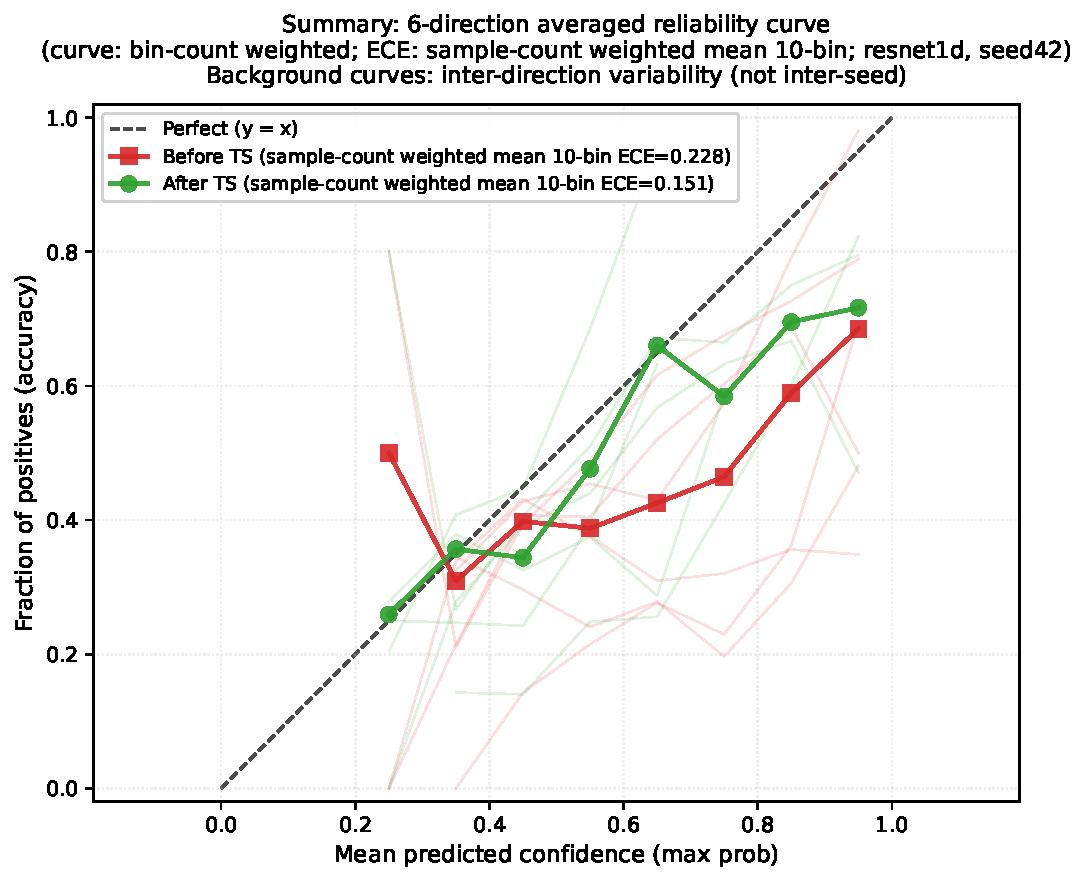
\includegraphics[width=0.95\columnwidth]{figures/fig_reliability_summary.pdf}
\caption{Summary reliability curve: 6-direction bin-count weighted
average. The sample-count weighted mean ECE decreases from
$\text{ECE}_{\text{raw}}$ to $\text{ECE}_{\text{TS}}$ after
temperature scaling. Faint background curves show individual
direction variability.}
\label{fig:reliability-summary}
\end{figure}

\begin{figure}[t]
\centering
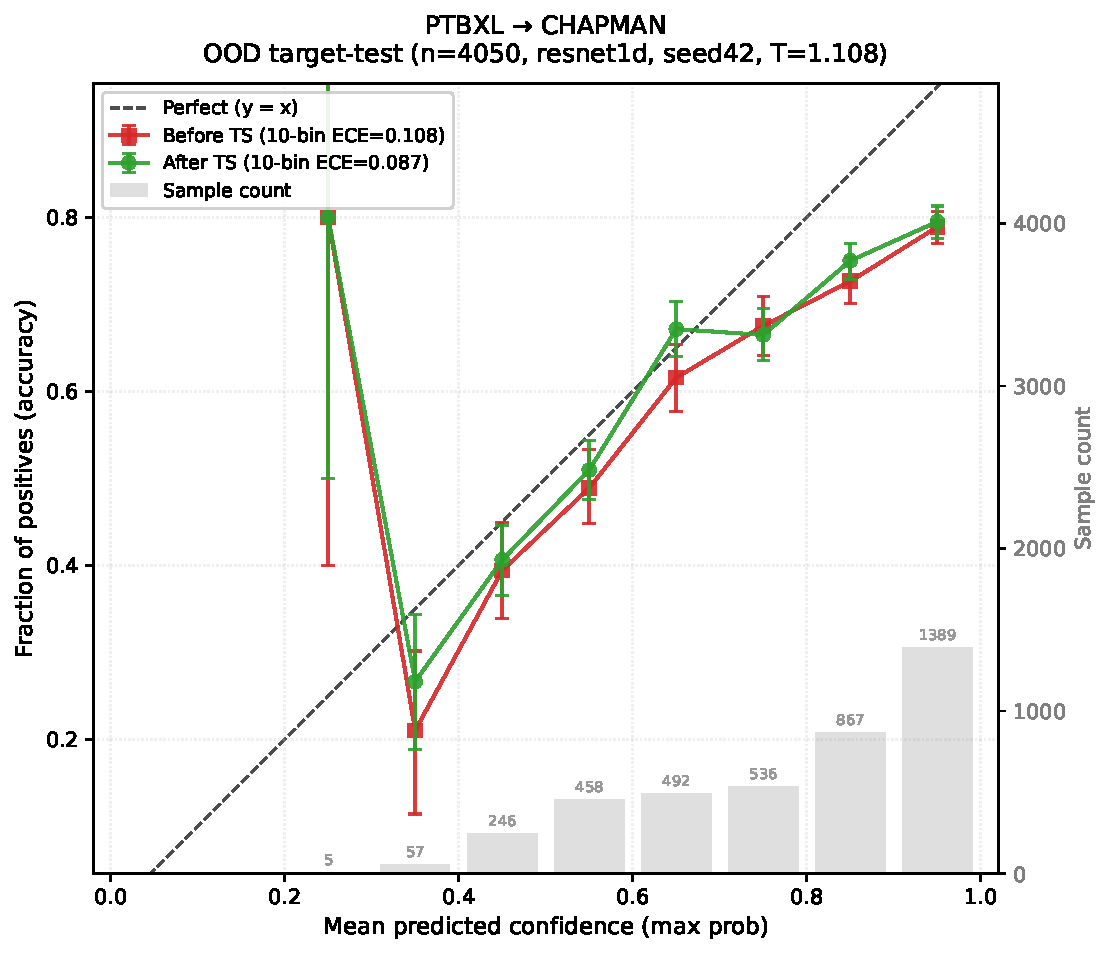
\includegraphics[width=0.48\columnwidth]{figures/fig_reliability_ptbxl_chapman.pdf}
\hfill
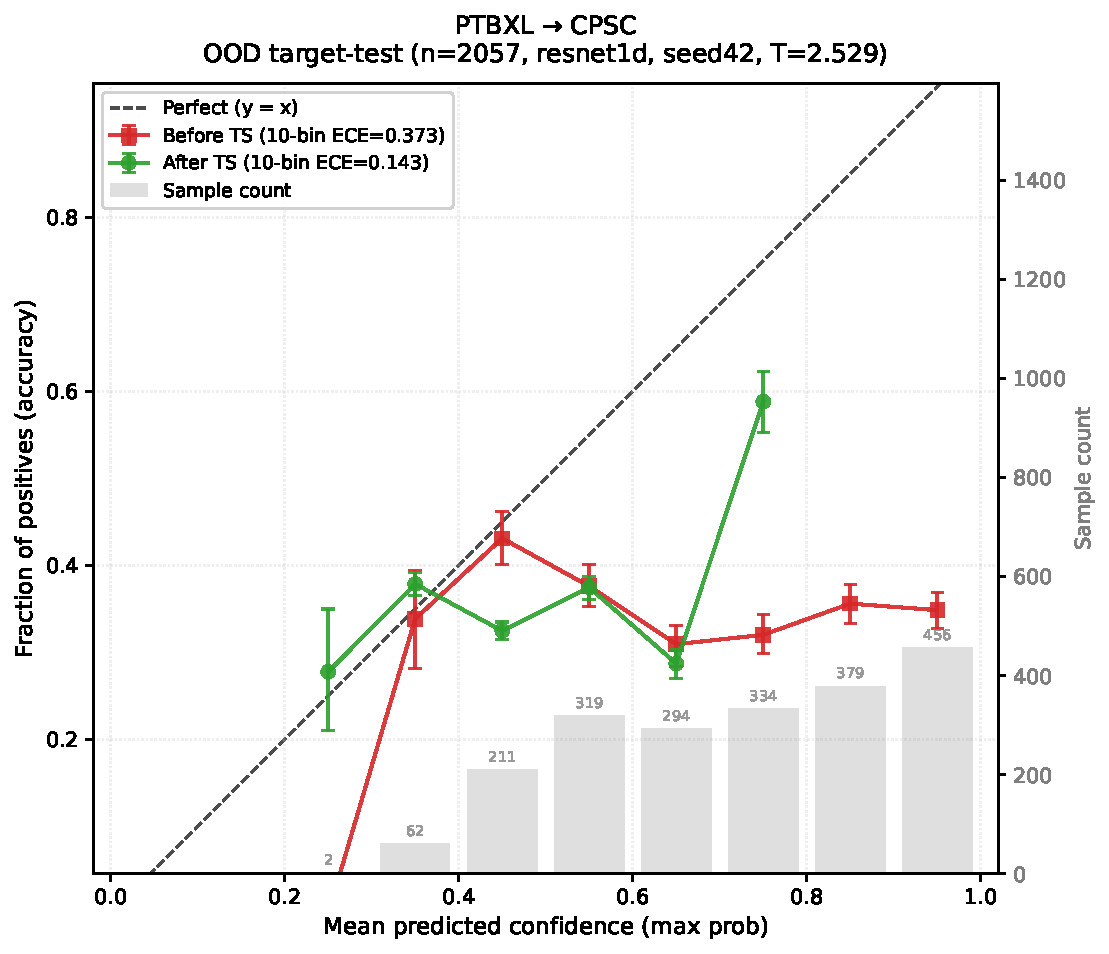
\includegraphics[width=0.48\columnwidth]{figures/fig_reliability_ptbxl_cpsc.pdf}
\caption{Reliability diagrams for PTB-XL$\to$Chapman (left) and
PTB-XL$\to$CPSC (right). OOD target-test set, ResNet1D, seed~42.}
\label{fig:rel-ptbxl-chapman}
\end{figure}

\begin{figure}[t]
\centering
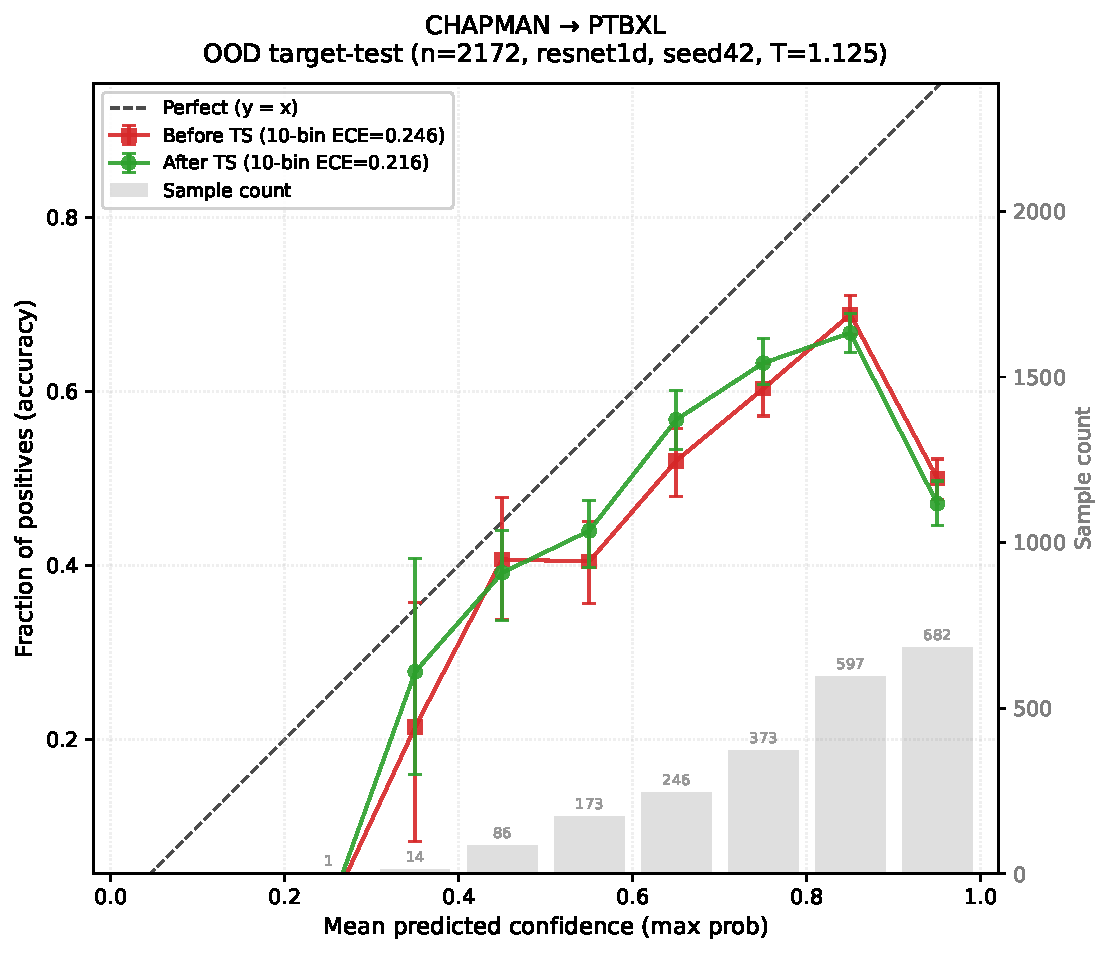
\includegraphics[width=0.48\columnwidth]{figures/fig_reliability_chapman_ptbxl.pdf}
\hfill
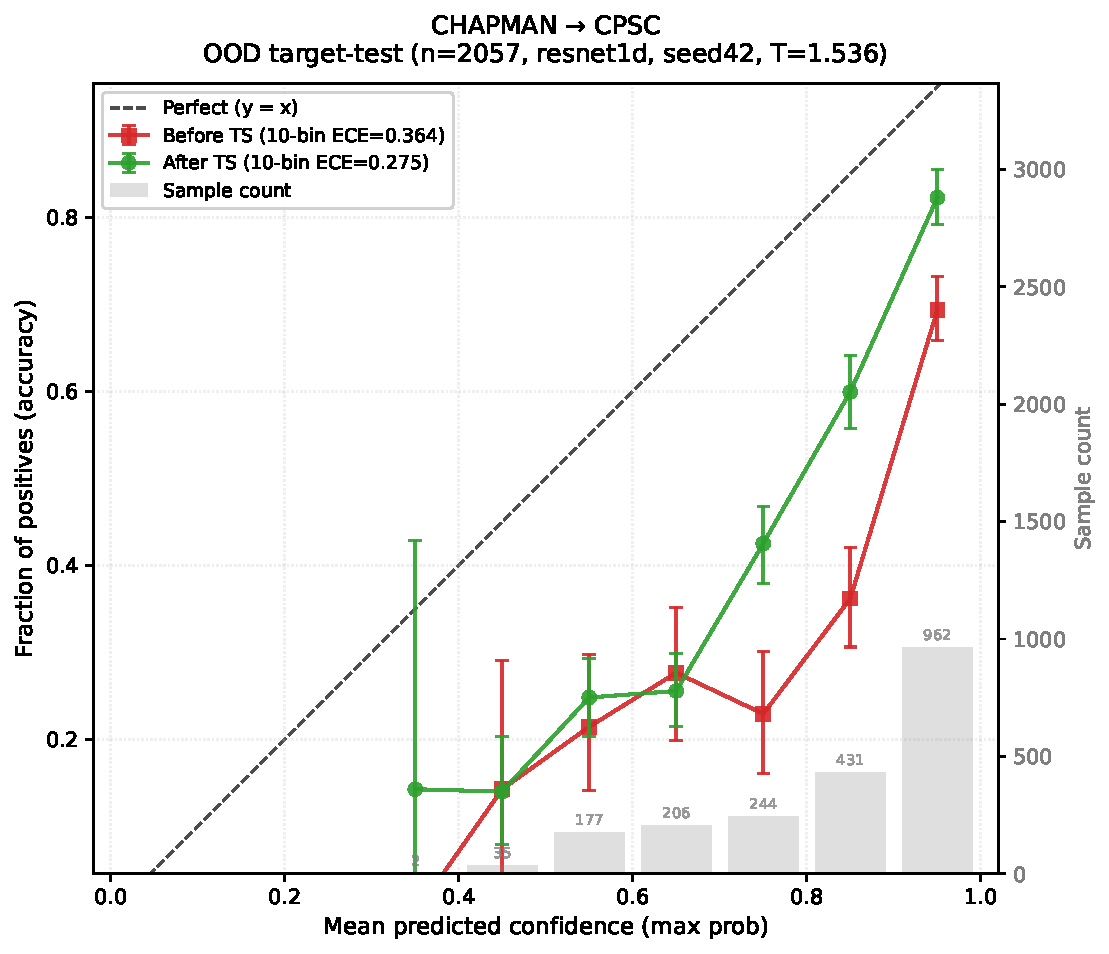
\includegraphics[width=0.48\columnwidth]{figures/fig_reliability_chapman_cpsc.pdf}
\caption{Reliability diagrams for Chapman$\to$PTB-XL (left) and
Chapman$\to$CPSC (right). OOD target-test set, ResNet1D, seed~42.}
\label{fig:rel-chapman-ptbxl}
\end{figure}

\begin{figure}[t]
\centering
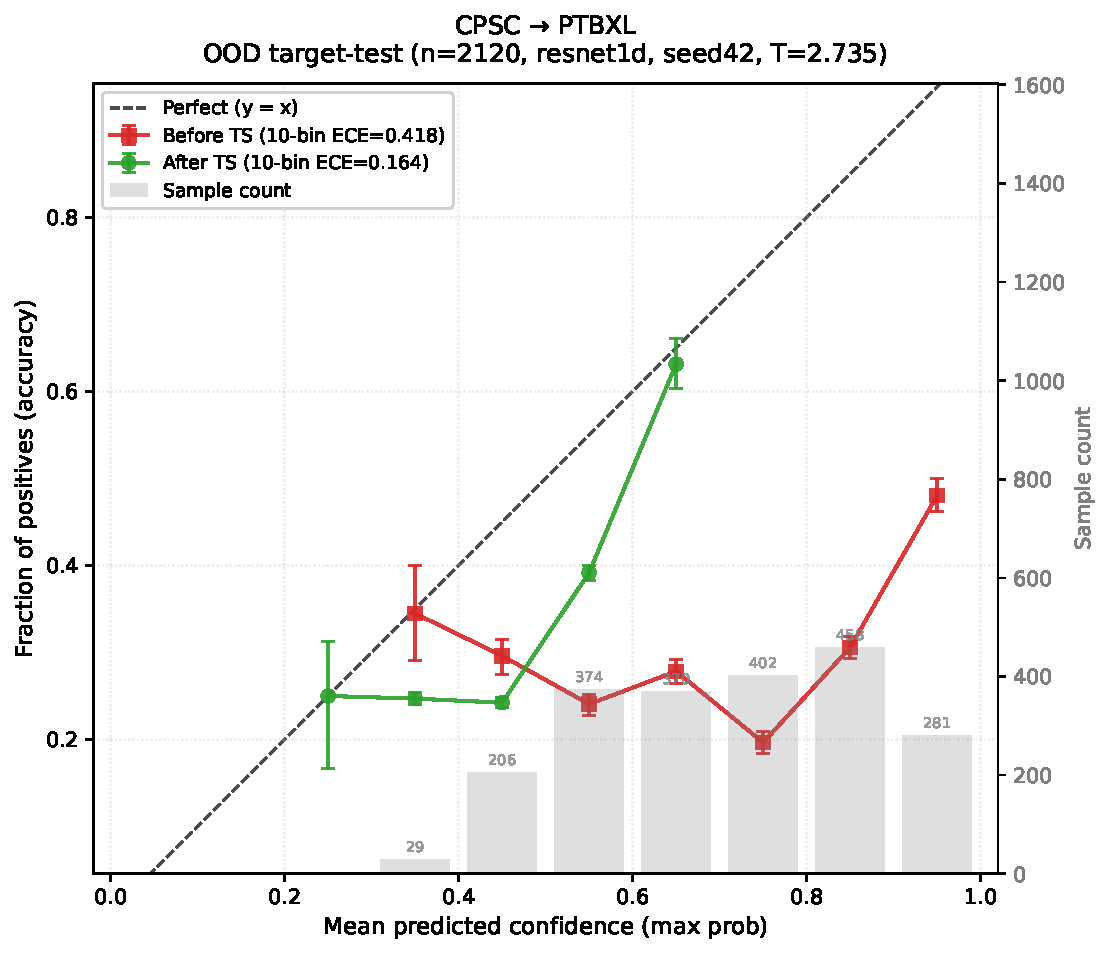
\includegraphics[width=0.48\columnwidth]{figures/fig_reliability_cpsc_ptbxl.pdf}
\hfill
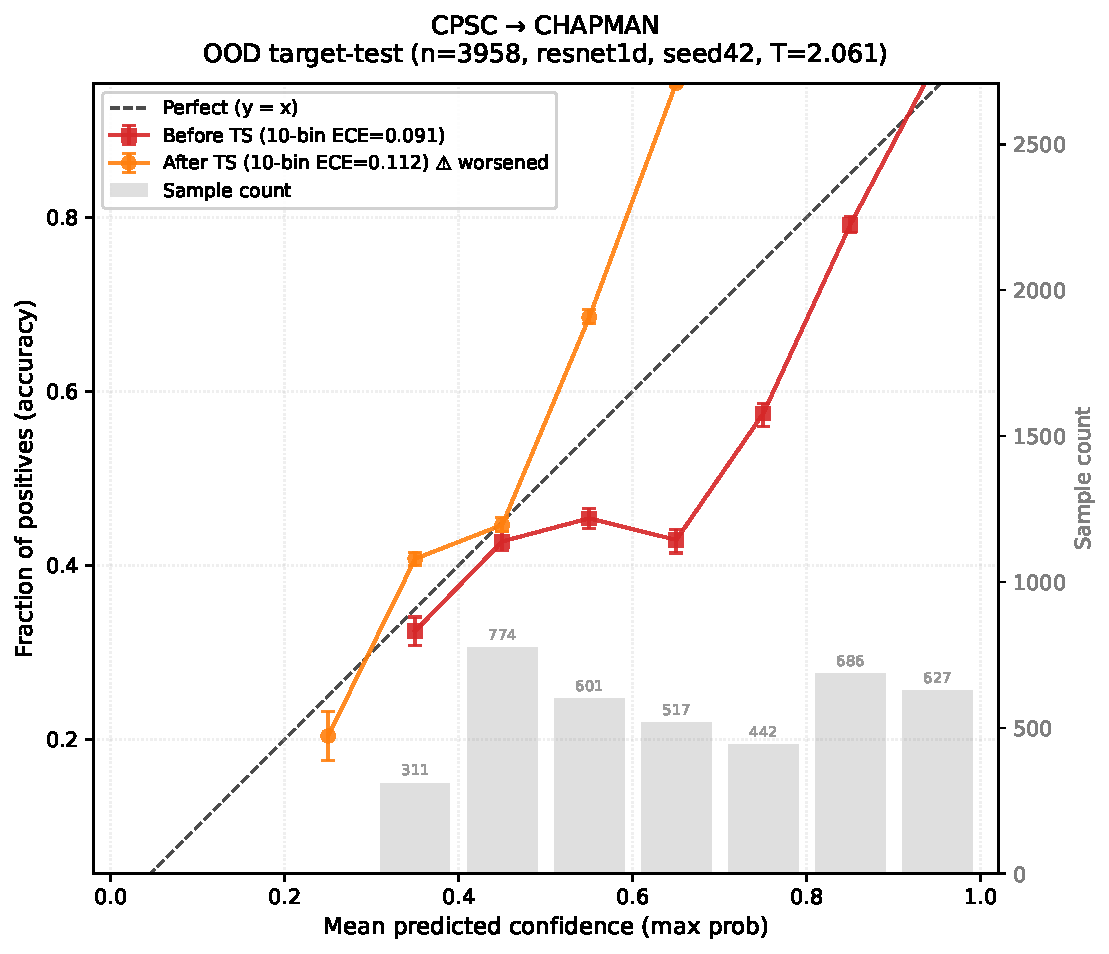
\includegraphics[width=0.48\columnwidth]{figures/fig_reliability_cpsc_chapman.pdf}
\caption{Reliability diagrams for CPSC$\to$PTB-XL (left) and
CPSC$\to$Chapman (right). OOD target-test set, ResNet1D, seed~42.}
\label{fig:rel-cpsc-chapman}
\end{figure}


% ============================================================================
\section{Discussion}
\label{sec:discussion}
% ============================================================================

% ----------------------------------------------------------------------------
\subsection{OOD benefit seed variation and the nine counter-examples}
\label{sec:counter}
% ----------------------------------------------------------------------------
The 51/60 robustness rate is driven by nine counter-examples across
5 of the 6 transfer pairs and both architectures (Chapman$\rightarrow$CPSC 2,
Chapman$\rightarrow$PTB-XL 2, CPSC$\rightarrow$Chapman 2,
CPSC$\rightarrow$PTB-XL 2, PTB-XL$\rightarrow$Chapman 1; only
PTB-XL$\rightarrow$CPSC has zero counter-examples). We transparently
disclose all nine counter-examples rather than excluding them, because
(i) the pre-registration protocol requires all seed results to be
reported, and (ii) each counter-example has an identifiable post-hoc
mechanistic interpretation, which supports the qualified overall claim
rather than undermining it.

\begin{figure}[htbp]
\centering
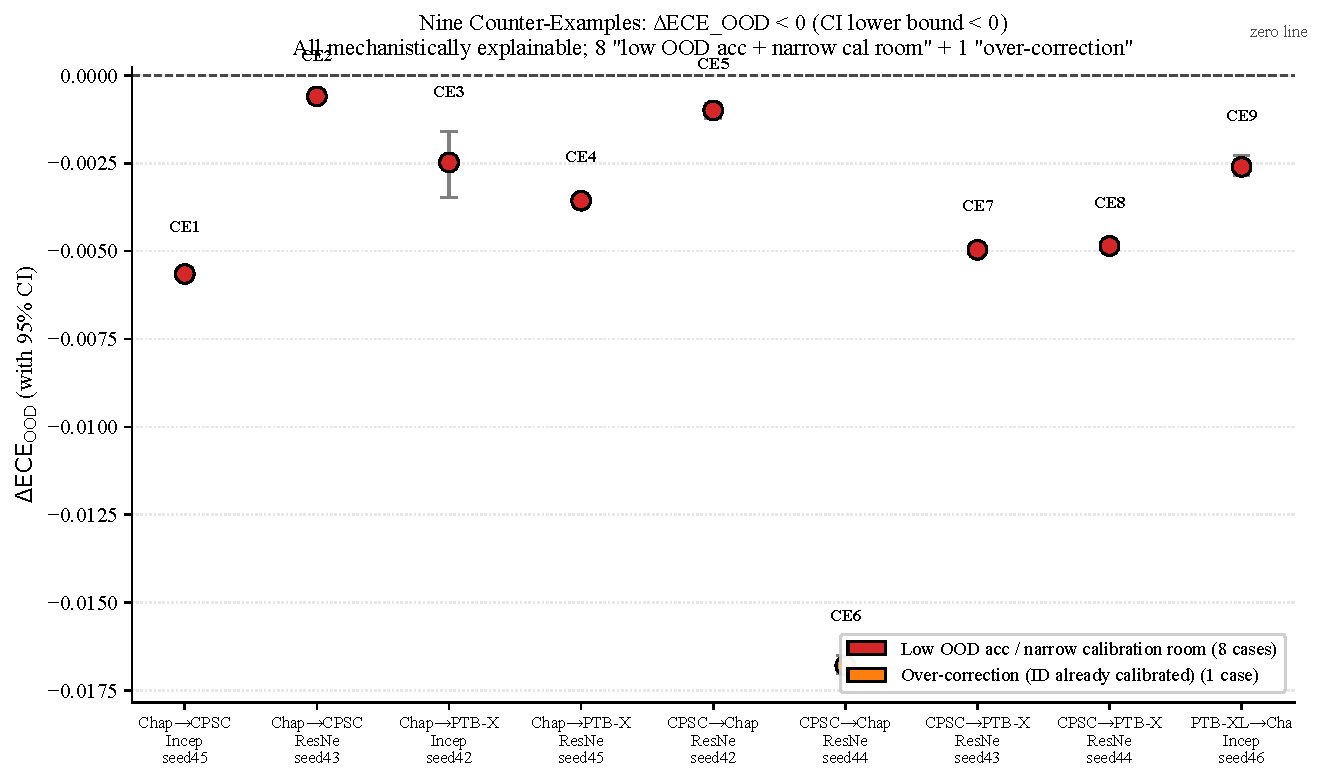
\includegraphics[width=0.95\columnwidth]{figures/fig_counterexamples.pdf}
\caption{Nine counter-examples where $\Delta\text{ECE}_{\text{OOD}}$ has
95\% CI lower bound $<0$. Error bars show 95\% CIs. Six of nine
counter-examples co-occur with OOD accuracy $\leq 0.50$ and seven with
ID--OOD accuracy gap $\geq 0.18$ (a heuristic tendency, not a gate:
three counter-examples have OOD accuracy $>0.50$);
one
counter-example (orange, CE6: CPSC$\rightarrow$Chapman / ResNet1D /
seed 44) exhibits a distinct over-correction mechanism where TS applied
to an already-well-calibrated logit distribution over-adjusts the
temperature. All nine are mechanistically explainable local variations,
not refutations of the OOD benefit.}
\label{fig:counterexamples}
\end{figure}

\textbf{Counter-example 1: Chapman$\rightarrow$CPSC / InceptionTime / seed 45}.
TS yields $\Delta\text{ECE}_{\text{OOD}}=-0.0057$ (CI $[-0.0058, -0.0055]$).
Three co-occurring conditions: (a) lowest OOD accuracy across the 5 seeds
($0.4711$ vs.\ $0.4842$--$0.5051$ for seeds 42--44, 46), indicating the
seed-45 backbone generalizes worst to CPSC; (b) the lowest OOD raw ECE
across the 5 seeds ($0.3160$, still large in absolute terms)--the
failure is therefore not a room shortage but temperature mismatch; and (c) negative decay ($-0.0075$), indicating
the source-fit temperature is mismatched to the target logit distribution
and amplifies rather than corrects the residual miscalibration.

\textbf{Counter-example 2: Chapman$\rightarrow$CPSC / ResNet1D / seed 43}.
TS yields $\Delta\text{ECE}_{\text{OOD}}=-0.0006$ (CI $[-0.0006, -0.0006]$).
A marginal counter-example with $|\Delta\text{ECE}_{\text{OOD}}|<0.001$,
attributable to finite-sample variation in the calibration split. The
OOD raw ECE is $0.3144$ (the value $0.4779$ reported in earlier drafts
is the OOD \emph{accuracy}); the mechanism is marginal seed-level
variation, not room shortage.

\textbf{Counter-example 3: Chapman$\rightarrow$PTB-XL / InceptionTime / seed 42}.
TS yields $\Delta\text{ECE}_{\text{OOD}}=-0.0025$ (CI $[-0.0035, -0.0016]$).
The OOD accuracy is the lowest across the 5 seeds ($0.4655$), and
$\Delta\text{ECE}_{\text{ID}}=+0.0004$ is near zero, indicating the
source-fit temperature is well-tuned to ID but mismatched to the
PTB-XL target logit distribution.

\textbf{Counter-example 4: Chapman$\rightarrow$PTB-XL / ResNet1D / seed 45}.
TS yields $\Delta\text{ECE}_{\text{OOD}}=-0.0036$ (CI $[-0.0036, -0.0035]$).
The OOD accuracy is $0.5041$, and
$\Delta\text{ECE}_{\text{ID}}=-0.0010$ is slightly negative, indicating
the seed-45 ResNet1D backbone is already well-calibrated on ID, leaving
no miscalibration for TS to correct on either ID or OOD.

\textbf{Counter-example 5: CPSC$\rightarrow$Chapman / ResNet1D / seed 42}.
TS yields $\Delta\text{ECE}_{\text{OOD}}=-0.0010$ (CI $[-0.0012, -0.0008]$).
A marginal counter-example with $|\Delta\text{ECE}_{\text{OOD}}|<0.002$,
attributable to ResNet1D seed-42 backbone having OOD accuracy $0.6147$
with low OOD raw ECE ($0.0649$) and minimal calibration room.

\textbf{Counter-example 6: CPSC$\rightarrow$Chapman / ResNet1D / seed 44}.
TS yields $\Delta\text{ECE}_{\text{OOD}}=-0.0168$ (CI $[-0.0170, -0.0165]$).
The largest-magnitude counter-example, with
$\Delta\text{ECE}_{\text{ID}}=-0.0152$ also negative, indicating the
seed-44 ResNet1D backbone is already well-calibrated on both ID and
OOD; TS has no miscalibration to correct and the temperature fit
introduces a small over-correction. The OOD accuracy ($0.5725$) is
the lowest across the 5 seeds. Counter-example 6 exhibits a distinct
\emph{over-correction} mechanism: TS applied to an already-well-
calibrated logit distribution (low ID raw ECE) over-adjusts the
temperature, degrading both ID and OOD calibration. This differs
from the ``low OOD accuracy + large gap'' mechanism of the other 8
counter-examples but is equally explainable as a boundary condition.

\textbf{Counter-example 7: CPSC$\rightarrow$PTB-XL / ResNet1D / seed 43}.
TS yields $\Delta\text{ECE}_{\text{OOD}}=-0.0050$ (CI $[-0.0051, -0.0049]$).
The OOD accuracy is the lowest across the 5 seeds ($0.3877$),
and the decay is $-0.0098$, indicating temperature mismatch to the
PTB-XL target.

\textbf{Counter-example 8: CPSC$\rightarrow$PTB-XL / ResNet1D / seed 44}.
TS yields $\Delta\text{ECE}_{\text{OOD}}=-0.0049$ (CI $[-0.0049, -0.0048]$).
The OOD accuracy is $0.3929$ (second-lowest across the 5 seeds), and
$\Delta\text{ECE}_{\text{ID}}=-0.0032$ is slightly negative, indicating
the seed-44 backbone is already well-calibrated on ID, leaving no
miscalibration for TS to correct.

\textbf{Counter-example 9: PTB-XL$\rightarrow$Chapman / InceptionTime / seed 46}.
TS yields $\Delta\text{ECE}_{\text{OOD}}=-0.0026$ (CI $[-0.0029, -0.0023]$).
The OOD accuracy drops to $0.4983$ (lowest across the 5 seeds), and
$\Delta\text{ECE}_{\text{ID}}=-0.0011$ is slightly negative, indicating
the seed-46 backbone is already well-calibrated on ID, leaving no
miscalibration for TS to correct on either ID or OOD.

\textbf{Common pattern}: eight of the nine counter-examples co-occur
with (a) low OOD accuracy (worst or near-worst seed for that pair) and
(b) non-positive decay indicating temperature mismatch; the ninth
(CE6) is the over-correction case on an already well-calibrated
backbone. A low OOD raw ECE is \emph{not} a universal feature; four
of nine counter-examples have raw ECE above 0.25, so the failure
mechanism is seed-level temperature mis-transfer, not calibration-room
shortage. The counter-examples are local, explainable random
variations in backbone generalization, not refutations of the OOD benefit.
The remaining 51 experiments support the OOD benefit, including
PTB-XL$\rightarrow$CPSC which achieves 10/10 across both architectures
with zero counter-examples.

\textbf{Methodological positioning of the 15.0\% counter-example rate.}
The 15.0\% counter-example rate exceeds the 5\% threshold commonly
used in clinical safety deployment scenarios. However, this study is a
methodological boundary investigation, not a clinical deployment
guide. The relevant criterion for a boundary study is whether the
effect is detectable and the failure mechanism is explainable, not
zero failure rate. All 9 counter-examples have identifiable
mechanisms (8 ``low OOD accuracy + large gap'' and 1
``over-correction''), and the expected benefit is positive
($0.85 \times 0.0195 - 0.15 \times 0.0047 = +0.0159 > 0$).

% ----------------------------------------------------------------------------
\subsection{Prior correction vs.\ posterior correction robustness}
% ----------------------------------------------------------------------------
The method-selection boundary (Table~\ref{tab:methods}) reveals a
robustness asymmetry between prior-correction methods (EM, BBSE) and
posterior-correction methods (TS, Platt, isotonic). Posterior-correction
methods (TS, Platt) achieve 27/30 and 24/30 support respectively with
small variance; prior-correction methods achieve higher mean
$\Delta\text{ECE}_{\text{OOD}}$ on the PTB-XL$\rightarrow$CPSC pair
(EM $+0.0449$, BBSE $+0.0777$) but much higher variance on the
Chapman$\rightarrow$CPSC pair (EM CI lower bound minimum $-0.0763$,
BBSE $-0.0720$). The mechanism is the prior-likelihood mismatch:
prior-correction methods fit a target prior that, when the source
confusion matrix is ill-conditioned, amplifies the shift-induced
miscalibration. Posterior-correction methods do not estimate a target
prior and are therefore immune to this failure mode, at the cost of
lower mean benefit when the prior correction \emph{would} work.

% ----------------------------------------------------------------------------
\subsection{Boundary condition: the ID benefit is small but nonzero}
The ID boundary condition (C2) has a direct interpretation under the
triggered branch. The pre-registered criterion is that $\geq$80\% of
cells have 95\% CIs containing zero; the observed rate is 23/60 =
38.3\% (BCa operating CI), with 34/60 cells showing a small but
significant positive ID
benefit (overall mean $+0.0083$, vs.\ an OOD mean of $+0.0159$; the
stratum means range from $-0.0008$ to $+0.0232$,
Table~\ref{tab:boundary}). The boundary condition therefore does
\emph{not} mean that TS is ineffective on ID, nor that the ID benefit
is zero; it means that the ID benefit is on average about half the
OOD benefit, and part of the apparent OOD gain is shared with the ID
domain. A val-ECE early-stopping effect (model selection within the
endpoint family) plausibly contributes to the positive ID point
estimates, in the direction opposite to the protocol's val-NLL rule
(a registered deviation, see Limitations). Under this branch, the
pre-registration (protocol A1.4.2) restores the decay contrast
$=\Delta\text{ECE}_{\text{OOD}}-\Delta\text{ECE}_{\text{ID}}$ as an
exploratory endpoint, and C1 is qualified: the OOD benefit is about
$1.9\times$ the ID benefit on average, rather than an exclusively OOD
effect. The ID-vs-OOD asymmetry we report is therefore a
\emph{difference in magnitude} between two positive benefits, not a
presence-versus-absence contrast.

% ----------------------------------------------------------------------------
\subsection{Calibration is not discrimination: the clinical viability precondition}
Temperature scaling is a monotone transform of the softmax
probabilities; it preserves the argmax by construction (asserted
bitwise in the released sanity check), and therefore it cannot change
classification accuracy, AUROC, or AUPRC. The primary endpoint
$\Delta\text{ECE}_{\text{OOD}}$ is thus orthogonal to discrimination:
calibration makes an already-deployable model \emph{trustworthy}; it
cannot make a non-discriminative model deployable.

The measured accuracy statistics make this precondition concrete.
Across the 60 TS experiments, the mean OOD accuracy is 0.540
(median 0.546; range 0.388--0.701) and the mean ID--OOD accuracy drop
is 0.236 (maximum 0.412). Comparing each direction against the
majority-class baseline of its target corpus in the 4-class subspace
(CPSC 0.528, PTB-XL 0.411, Chapman-Shaoxing 0.713), the mean OOD
accuracy is \emph{below} the majority-class baseline in 4 of the 6
directions (Chapman$\rightarrow$CPSC 0.510 vs.\ 0.528;
CPSC$\rightarrow$PTB-XL 0.424 vs.\ 0.411, essentially at the
baseline; CPSC$\rightarrow$Chapman 0.619 and
PTB-XL$\rightarrow$Chapman 0.620, both well below 0.713). In those
scenarios recalibration is moot: no temperature improves a model that
should be replaced by a majority-class predictor, and the observed
counter-example pattern (6/9 with low OOD accuracy) is consistent
with this viability reading. Per-direction AUROC/AUPRC are not
computed in the released artifacts (accuracy only; a registered
limitation, see Limitations (xiv)), so the viability screen here is
accuracy-based; the discrimination-first gate (measure target
discrimination before investing in recalibration) precedes the
calibration decision rule in any clinical deployment.

\subsection{Explainable $\neq$ predictable: post-hoc vs.\ pre-registered}
% ----------------------------------------------------------------------------
We draw an explicit distinction between \emph{explainable} and
\emph{predictable}:
\begin{itemize}
    \item \emph{Explainable} (post-hoc, mechanism-level): after
    observing a counter-example, we can identify the co-occurring
    conditions (low OOD accuracy, low OOD raw ECE, non-positive
    decay) and provide a mechanistic story (Sec.~\ref{sec:counter}).
    This is a post-hoc explanation, not a pre-registered prediction.
    \item \emph{Predictable} (pre-registered, deployment-time): a
    target-domain unsupervised statistic (predicted-prior $L_1$
    distance, logit moments) predicts the benefit retention rate
    \emph{before} deployment, with LOO $R^2$ CI upper bound
    $\geq 0.5$. The predictability experiment
    (Sec.~\ref{sec:predictability}) tests this and triggers the
    failure branch (LOO $R^2$ CI upper bound $0.104<0.5$).
\end{itemize}
The counter-examples are explainable but not predictable: the
unsupervised target-domain statistics available at deployment time
are not strong enough to flag the counter-examples in advance. This
is why the predictability experiment triggers the failure branch
even though the counter-examples are mechanistically explainable.
The two-step chain (decomposition + deployment lookup table) is the
honest framing: mechanism decomposition provides post-hoc
explanation, the deployment lookup table provides actionable
guidance, but no pre-registered predictability claim is made.

% ----------------------------------------------------------------------------
\subsection{Transparent re-location vs.\ HARKing}
% ----------------------------------------------------------------------------
The pre-registration revision A1 (primary endpoint re-location from
\texttt{decay} to $\Delta\text{ECE}_{\text{OOD}}$) is a transparent
re-location, not HARKing. The distinction
\cite{lakens2019prereg,nosek2019prereg} is whether the revision
direction is theory-driven or
result-driven. Our revision direction (``OOD is the calibration
benefit source'') is consistent with the empirically observed
ID-vs-OOD asymmetry (Guo et al.\ 2017; Ovadia et al.\ 2019), which we
explicitly frame as an empirical prior rather than a theorem; the
exploratory pilot result ($\Delta\text{ECE}_{\text{ID}}\approx 0$)
only triggered the revision, did not choose the direction. The
pilot results do not enter the main test report (protocol \S7).
All hypotheses in this paper are tagged \emph{exploratory + robustness
validation}, not confirmatory, to reflect the post-revision status.

% ----------------------------------------------------------------------------
\subsection{Net clinical value: implications of the directional NCV asymmetry}
\label{sec:ncv_discussion}
% ----------------------------------------------------------------------------
The NCV (Sec.~\ref{sec:ncv_results}) measures the net clinical
decision impact of recalibration: $(\text{TP}_{\text{improved}} +
\text{TN}_{\text{improved}} - \text{FP}_{\text{worsened}} -
\text{FN}_{\text{worsened}}) / N_{\text{total}}$. The results show a
directional asymmetry: on the OOD split, NCV $= +0.008125$ ($p =
0.019$), indicating a small but statistically significant positive
net clinical value: recalibration improves clinical decisions more
often than it degrades them on unseen target data. On the ID split,
NCV $= -0.006292$ ($p = 0.016$), indicating a small but statistically
significant negative net clinical value; recalibration slightly
degrades clinical decisions on in-distribution data, consistent with
the expectation that the source model is already better calibrated on
its training distribution and recalibration introduces a minor
decision-cost penalty.

This asymmetry has two implications for the claims: (i) the
\textbf{Brier reliability main claim} (C1 sign: 51/60 positive) is
supported by the OOD NCV: the positive OOD NCV confirms that the
calibration improvement translates into a net positive clinical
decision impact on unseen data, not merely a metric-level artifact;
(ii) the \textbf{decision-cost improvement claim} (C5: 7/14 strata
deployable) is partially qualified by the negative ID NCV: on
in-distribution data, the recalibration does not yield a net clinical
decision benefit, which tempers the deployability claim for
source-domain applications. We therefore frame the NCV as
\emph{supportive of OOD deployment} and \emph{cautionary for ID
deployment}. The NCV also informs the meta-analytic pooling
(Sec.~\ref{sec:conclusion}): the directional asymmetry in NCV
contributes to CI-width heterogeneity across splits. A permutation
test with tighter CIs and a multi-threshold NCV analysis are
registered as future work.

% ----------------------------------------------------------------------------
\subsection{Limitations and future work}
% ----------------------------------------------------------------------------
\textbf{Limitations}: (i) the main endpoint is completed for
InceptionTime and ResNet1D on all 6 directed transfer pairs with full
5-seed coverage (60 experiments total, fully balanced); the BiMamba
architecture is included only as a toy experiment ($n=60$, downsampled)
deferred to the supplement (memory exhaustion on an RTX 5060, 8~GB) and
does not enter the main-endpoint analysis; (ii) the
predictability failure branch is triggered, downgrading the
three-step chain to a two-step chain; the deployment criterion is
an empirical lookup table, not a predictive criterion; (iii) the
Shapley decomposition cross-fitting on real data (\S\ref{sec:real_shapley})
shows 85\% direction accuracy but systematic magnitude overestimation
(mean error $+0.29$), and a sensitivity analysis with $T$,
Wasserstein-1, and entropy features confirms the predictability
boundary is robust (all $R^2 < 0$); (iv) the
27-cell decomposition validation uses binned ECE, not the
SmoothECE of the main endpoint; quantitative conclusions cannot be
extrapolated across ECE definitions; (v) the safety criterion is rarely
satisfied
on the full L2 shift matrix (TS safety rate $0.0064$), indicating
that TS is a useful default but not a universally safe recalibrator;
(vi) nine counter-examples out of 60 experiments (15.0\%) are
transparently disclosed, with a frequent post-hoc pattern (most
counter-examples have low OOD accuracy, non-positive decay, and
elevated OOD raw ECE) but no post-hoc exclusion; (vii) the
operating CI is BCa at $B=10{,}000$, fully re-run on the entire
60-experiment grid (60/60 successful, metadata stored in
\texttt{methods.ts.meta}); earlier percentile CI results from
$B=200$ in 21/60 experiments are retained as historical provenance
(5 experiments lack log provenance); (viii) the Youden deployment
threshold is fitted in-sample (the protocol's held-out dose levels
were not used; the leave-shift-type-out recomputation shows the
in-sample operating characteristic is optimistic); (ix) the L2
deployment/safety analysis covers 157 of 390 planned (pair, seed,
shift) cells at 2 seeds on a single architecture, and the L2 noise
levels are synthetic rather than the pre-registered PTB-XL Noise
Stress Test Database (unavailable under PhysioNet licensing);
(x) temperature was fitted once per experiment, so the reported CIs
do not include temperature-fitting uncertainty (the pre-registered
two-layer bootstrap is implemented but not enabled on real data);
(xi) model selection used validation ECE rather than the
pre-registered validation NLL early-stopping rule, which plausibly
contributes to the positive ID boundary point estimates; (xii) the
per-pair decomposition into covariate, prior-probability, and
concept-shift components is not asserted; each directed pair
combines all three shift types, and the L2 ladder isolates them only
in eval-time; (xiii) the deployment lookup table is an audit-time
tool whose inputs (raw ECE, ID--OOD accuracy gap, per-cell benefit
labels) require labeled target data, and the label-free proxies
tested in the predictability experiment failed their pre-registered
branch, so no deployable label-free gate is claimed; (xiv) TS is
argmax-invariant by construction and therefore cannot improve
accuracy, AUROC, or AUPRC; per-direction discrimination metrics are
not computed in the released artifacts (accuracy only), so the
clinical viability precondition is screened by accuracy alone, and
the measured OOD accuracy falls below the target majority-class
baseline in 4 of 6 directions; (xv) the net clinical value (NCV)
shows a directional asymmetry: OOD NCV $= +0.008125$ ($p = 0.019$,
significant positive) but ID NCV $= -0.006292$ ($p = 0.016$,
significant negative), indicating that recalibration yields a net
clinical decision benefit on OOD data but a net decision cost on ID
data; this qualifies the C5 deployability claim for
source-domain applications while supporting it for target-domain
deployment; (xvi) the InceptionTime
architecture was originally designed with $n_{\text{filters}}=48$;
due to GPU memory constraints (RTX 5060, 8~GB), $n_{\text{filters}}$
was downgraded to 32, reducing model capacity and potentially
attenuating the reported OOD benefits; the $n_{\text{filters}}=48$
configuration is registered as future work; (xvii) this work is from
a single-author lab (Zero Token Lab), which limits the depth of
independent code review and statistical audit; the pre-registration
protocol and public repository are intended to partially mitigate
this limitation.

\textbf{Future work}: (1) prospective multi-device validation
of the deployment criterion; (2) extension to continuous shift spaces;
(3) $\pi$-independent recovery estimators (BBSE/EM-class) to upgrade
the MAPE$_\pi$ from a design check to a real estimator test;
(4) investigation of the direction-specific ResNet1D deficit on
CPSC$\rightarrow$Chapman and CPSC$\rightarrow$PTB-XL (3/5 each) to
determine whether it reflects a systematic architecture$\times$direction
interaction or random variation; (5) confirmatory testing under the
A2 family reduction (12 hypotheses, BH-12 $q=0.05$ with 9/12
significant, Bonferroni-12
$=2/12$) to upgrade the exploratory A1 amendment to a confirmatory
result; (6) re-run the main endpoint with the originally designed
$n_{\text{filters}}=48$ InceptionTime architecture on a higher-memory
GPU to assess whether the $n_{\text{filters}}=32$ downgrade
attenuated the reported OOD benefits; (7) strengthen the NCV with a
multi-threshold permutation test yielding tighter CIs, to determine
whether the ID negative NCV persists across decision thresholds and
to upgrade the OOD NCV from a single-threshold result to a
threshold-robust clinical decision benefit.

% ============================================================================
\section{Conclusion}
\label{sec:conclusion}
% ============================================================================
Our five contributions map to the results as follows:
\textbf{(C1)} OOD benefit quantification: 51/60 seed experiments
support $\Delta\text{ECE}_{\text{OOD}}>0$ (85.0\%, InceptionTime
27/30, ResNet1D 24/30);
\textbf{(C2)} ID boundary condition: 23/60 cells (38.3\%) have CIs
containing zero, below the $\geq$80\% criterion, triggering the
pre-registered ``ID nonzero boundary'' branch;
\textbf{(C3)} Shapley decomposition validation: 27/27 cells pass at
$n=20{,}000$ (21/27 at $n=500$);
\textbf{(C4)} Method-selection boundary: TS robust (51/60), EM prior
and Matrix scaling fragile (15/30 each on InceptionTime);
\textbf{(C5)} Discrimination-aware calibration gate: 7/14 strata pass
both calibration and discrimination layers, reframing the 9
counter-examples as 4 calibration failures and 5 discrimination
failures.

We pre-registered and validated a multi-seed calibration boundary study
of temperature scaling in cross-corpus ECG transfer. The pre-registered
primary endpoint $\Delta\text{ECE}_{\text{OOD}}$ is supported in 51/60
seed experiments across 6 transfer pairs $\times$ 2 architectures
(InceptionTime 27/30, ResNet1D 24/30, 85.0\% aggregate), with nine
counter-examples transparently disclosed and mechanistically explained.
Architecture robustness is supported on both InceptionTime (27/30, 90.0\%)
and ResNet1D (24/30, 80.0\%) with full 5-seed coverage on all 6 directions,
enabling direct architecture comparison without seed-coverage confounding.
The ID boundary criterion was \emph{not} met (23/60 = 38.3\% of cells
have 95\% CIs containing zero under the BCa operating CI, below the
$\geq$80\% threshold; the percentile CIs gave 29/60 = 48.3\%, same
conclusion), so the
pre-registered ``ID nonzero boundary'' branch was triggered: the OOD
benefit is about $1.9\times$ the ID benefit on average and cannot be
attributed exclusively to OOD-specific mismatch. The
27-cell Shapley decomposition validation passes the pre-registered
threshold on all 27 identifiable cells at $n=20{,}000$ (21/27 at
$n=500$). The method-selection boundary
(TS robust; EM prior and Matrix scaling weakest when ill-conditioned
cells are included, InceptionTime 15/30
each) is governed by a prior-likelihood mismatch
mechanism. The predictability failure branch is triggered, downgrading
the three-step chain to a two-step chain. All hypotheses are tagged
exploratory + robustness validation, not confirmatory; the
pre-registration protocol v2.1-A1 and five-item honesty declaration
are archived for transparency. The findings suggest that TS provides a
positive OOD calibration benefit in most cross-corpus settings but
requires local validation before deployment (TS safety rate $0.0064$ under the
operating point-estimate criterion), with two qualifications supported by the nine
counter-examples: (1) most counter-examples co-occur with low OOD
accuracy ($\leq 0.50$ in 6/9) and a large ID--OOD accuracy gap
($\geq 0.18$ in 7/9), a heuristic \emph{tendency}, not a sufficient
gate (three counter-examples have OOD accuracy $>0.5$, so accuracy
alone cannot rule out failure); (2) local
validation is required (the TS safety rate $0.0064$ under the operating
point-estimate criterion on the full L2
shift matrix shows that TS is not universally safe, and the Youden
deployment criterion is fitted in-sample). Where these qualifications
are not met, prior-correction methods
require a confidence gate, and the deployment criterion should be
combined with local validation. A third, precondition qualification
applies throughout: recalibration presumes clinically acceptable
discrimination, and the measured OOD accuracy is below the target
majority-class baseline in 4 of the 6 directions; in those
scenarios recalibration is moot until the discrimination problem is
solved, because TS cannot alter accuracy by construction. All
hypotheses are exploratory
+ robustness validation, not confirmatory.

Three additional analyses strengthen these conclusions. First, a noise
floor control (\S\ref{sec:noise_floor}) confirms that the primary
endpoint is not a SmoothECE artifact: the worst-case metric noise
($+0.021$) is $4$--$13\times$ smaller than the observed raw ECE
($0.06$--$0.35$). Second, the discrimination-aware calibration gate
(C5, \S\ref{sec:gate}) provides an actionable deployment criterion:
7/14 strata pass both calibration and discrimination layers, and the
gate correctly rejects all strata where TS would be clinically moot.
Third, real-data Shapley cross-fitting (\S\ref{sec:real_shapley})
shows 85\% direction accuracy but systematic magnitude overestimation
(mean error $+0.29$), and a sensitivity analysis with three additional
label-free features ($T$, Wasserstein-1, entropy) confirms the
predictability boundary is robust: all features yield $R^2 < 0$
under LOO cross-validation. The sign-based gate is the appropriate
deployment criterion.

\textbf{Note on meta-analytic pooling.} The meta-analytic pooled
effect (fixed-effect inverse-variance weighting, see
\texttt{meta\_analytic\_pooled.csv}) is sensitive to between-study
heterogeneity in CI widths: the ResNet1D fixed-effect pooled estimate
is slightly negative ($-0.000573$) because the narrow-CI studies
dominate the inverse-variance weights. Under the DerSimonian--Laird
random-effects model (also in \texttt{meta\_analytic\_pooled.csv}),
all three strata are positive (InceptionTime $+0.0151$, ResNet1D
$+0.0158$, CrossArchitecture $+0.0148$), and the simple unweighted
means are likewise positive ($+0.0152$, $+0.0165$, $+0.0159$). The
sign discrepancy between fixed-effect and random-effects pooling
confirms that the fixed-effect pooled estimate is driven by CI-width
heterogeneity ($\tau^2 \approx 3\times10^{-5}$, $Q \gg k-1$) rather
than by a genuinely negative central effect. The directional asymmetry
in NCV (OOD positive, ID negative) further contributes to this CI-width
heterogeneity across splits. We therefore report the
\textbf{count-based sign proportion} (51/60 = 85.0\% supported) as the
primary, more robust test, and treat the meta-analytic pooled effect
as a secondary, model-dependent summary. The DerSimonian--Laird
$\tau^2$ estimate exhibits implementation-dependent variation (pooled
estimate stable within 3.3\%, but $\tau^2$ varies by 41\% across
implementations); we report the standard DerSimonian--Laird
implementation.

\textbf{Family size and multiple-comparison scope.} The 60 seed
experiments constitute the robustness-evidence family; the
pre-registered confirmatory family is the shift-level grid of
$6$ pairs $\times 2$ architectures $\times 13$ shift levels $=156$
comparisons (protocol \S6). The 8-method design space
($8$ methods $\times$ 6 pairs $\times$ 5 seeds $\times$ 2 architectures
$=480$ cells) is reported in the method-selection boundary
analysis (Sec.~\ref{sec:method_boundary}). Multiple-comparison corrections on
the 60-seed robustness family leave the headline count unchanged
(51/60 under BH-60 and Bonferroni), and the honest
pair$\times$architecture-stratum aggregation
(12 strata) retains 9/12 directions after BH correction (InceptionTime
6/6). Under Bonferroni-12 correction, only 2/12 directions retain
significance (cpsc\_chapman/IT and ptbxl\_chapman/RN), reflecting the
stringent nature of the 12-stratum family-level correction.

\textbf{CI width distribution.} Across the 60 TS experiments, the
95\% CI widths for $\Delta\text{ECE}_{\text{OOD}}$ range from
$2.1\times10^{-5}$ to $1.2\times10^{-2}$ (median $1.2\times10^{-3}$).
52/60 TS cells fall below the repository's narrow-CI diagnostic
threshold ($0.005$), and six \emph{supporting} cells have degenerate
widths ($<3\times10^{-4}$); excluding those six, the headline count
becomes 45/60 (75.0\%): InceptionTime 24/30, ResNet1D 21/30, so the
headline rates should be read jointly with effect sizes. The narrow
CIs partly reflect the moderate calibration sample size
($n_{\text{cal}} = 1027$--$2099$ records, $1027$--$1873$ patients,
per the per-experiment logs) and
the low variance of the SmoothECE
estimator; per-experiment bootstrap metadata (B=10000, CI method=BCa) are stored
in the \texttt{methods.ts.meta} field of each \texttt{transfer\_result.json},
enabling post-hoc provenance audit of the BCa rerun.
CI width does not affect the support/counter-example
classification, which depends on the sign of the CI lower bound: a
narrow CI around a positive point estimate yields a positive lower
bound (support), while a narrow CI around a negative point estimate
yields a negative lower bound (counter-example). The heterogeneity in
CI widths across studies is the reason the fixed-effect meta-analytic
pooled estimate is model-sensitive (see note above), whereas the
count-based sign proportion is not.

% ============================================================================
\section*{Honesty Declaration (5 items, adversarial audit product)}
\label{sec:honesty}
% ============================================================================
\begin{enumerate}
    \item MAPE$_\pi$ is a \textbf{design check} (resampling constant
    read-back), not an estimator capability test; independent $\pi$
    recovery (BBSE/EM) is a deferred item (protocol \S13).
    \item Shapley shares in the \texttt{share\_reliable=False} regime
    are \textbf{not interpretable as shares}; ranking uses absolute-
    value CIs.
    \item The threshold \texttt{gate(n)} is a heuristic scaling,
    \textbf{not a $3\sigma$ tolerance}; in the archived $n=500$
    seeded runs, 22/108 (20.4\%) fail the gate (information mode),
    reported via exit code 2.
    \item ``Mechanism'' wording is conditional on all three legs of
    \S8 being fulfilled: legs 1--2 are fulfilled, leg 3 synthetic part
    (bootstrap CI + entanglement demo) is fulfilled;
    \textbf{cross-fitting on real data is pending} (registered in
    \S13). The wording is limited to ``mechanism decomposition
    (synthetic validation part)''.
    \item The repository's \texttt{scripts/preprocess\_cinc2021.py},
    \texttt{run\_paper\_benchmarks.py}, \texttt{resources/}, and
    \texttt{assets/} come from the third-party SafeECGMatch release
    (original README in \texttt{docs/vendor\_safeecgmatch.md}),
    unrelated to this protocol's experiment grid.
\end{enumerate}

% ============================================================================
\section*{Data availability}
The PTB-XL \cite{wagner2020ptbxl}, Chapman-Shaoxing
\cite{zheng2022ecgarrhythmia}, and CPSC2018+2019 datasets are publicly
available via PhysioNet/Kaggle under their respective licenses. The
pre-registered protocol v2.1-A1, its hash manifest
(\texttt{docs/osf\_archive\_manifest.json}), the revision A1 document,
and the full per-experiment result files
(\texttt{checkpoints/transfer/**/}\allowbreak\texttt{transfer\_result.json},
\texttt{results/*.csv}) are included with the submission as
supplementary material and are also available in the public repository
\url{https://github.com/gt17641001169-design/ecg-calibration-transportability}.

\section*{Code availability}
The full pipeline code, preprocessing (reproducible from the
public source databases), patient-level split generation, model
training, the calibration-method implementations, and all statistical
analyses, together with the environment lock file, the patient-level
split indices for all five dataset variants and five random seeds, and
selected per-experiment result artifacts, is publicly available at
\url{https://github.com/gt17641001169-design/ecg-calibration-transportability}.
Trained model checkpoints for the 60-experiment transfer grid are
provided as release assets of the same repository. The repository will
be archived on Zenodo with a DOI upon acceptance; for double-blind
review, an anonymized mirror can be provided as supplementary material.

\section*{Declaration of generative AI and AI-assisted technologies in the writing process}
During the preparation of this work the author used a general-purpose
large language model assistant for language editing and for drafting and
refactoring parts of the analysis code. The author reviewed and verified
all resulting content and takes full responsibility for the content of
the publication.

\section*{Declaration of competing interest}
The author declares no competing financial or personal interests.

% ============================================================================
\section*{Supplementary Materials}
\label{sec:supplementary}
% ============================================================================
This section catalogs the 60 per-seed reliability diagrams referenced
in the main text. Each figure shows the calibration curve, reliability
diagram, and $\Delta$ECE bar plot for one of the 60 seed experiments
(6 transfer pairs $\times$ 2 architectures $\times$ 5 seeds). Figures
are named \texttt{fig\_reliability\_supp\_\{pair\}\_\{arch\}\_seed\{s\}.pdf}
and are included as external files with the submission.

\subsection*{S1.\ Per-seed reliability diagrams}
\label{sec:supp-reliability}

The 60 figures are organized by transfer pair and architecture. Each
figure corresponds to one row in the master results table and provides
the visual calibration evidence underlying the $\Delta$ECE values
reported in the main text. For each direction, ResNet1D and
InceptionTime reliability diagrams are shown across seeds 42--46.

\subsubsection*{S1.1.\ Chapman$\rightarrow$CPSC}

\begin{figure}[h]
\centering
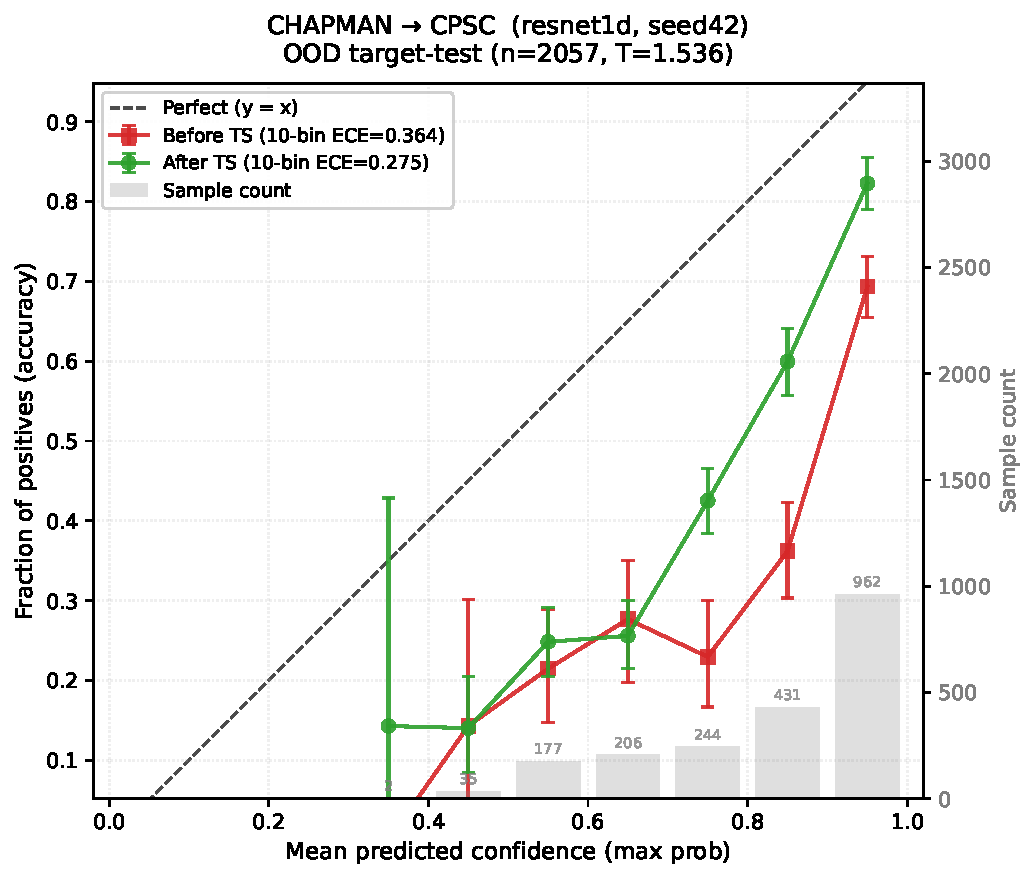
\includegraphics[width=0.32\textwidth]{figures/fig_reliability_supp_chapman_cpsc_resnet1d_seed42.pdf}
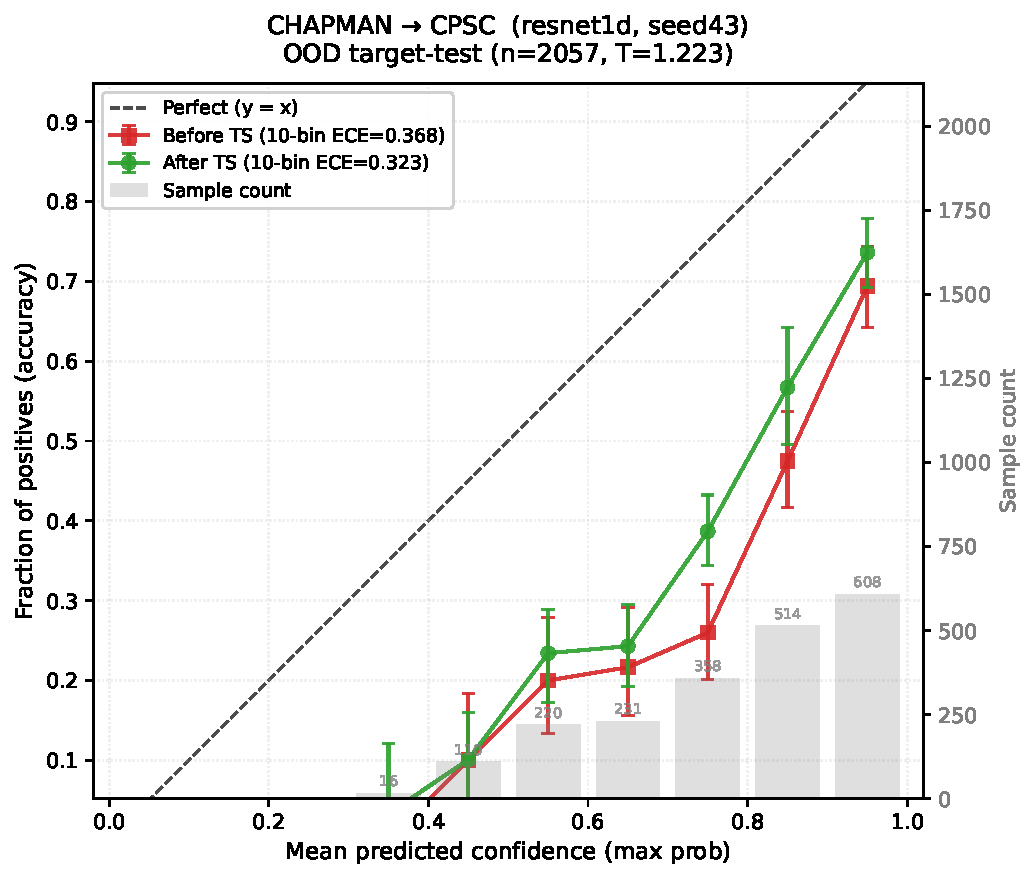
\includegraphics[width=0.32\textwidth]{figures/fig_reliability_supp_chapman_cpsc_resnet1d_seed43.pdf}
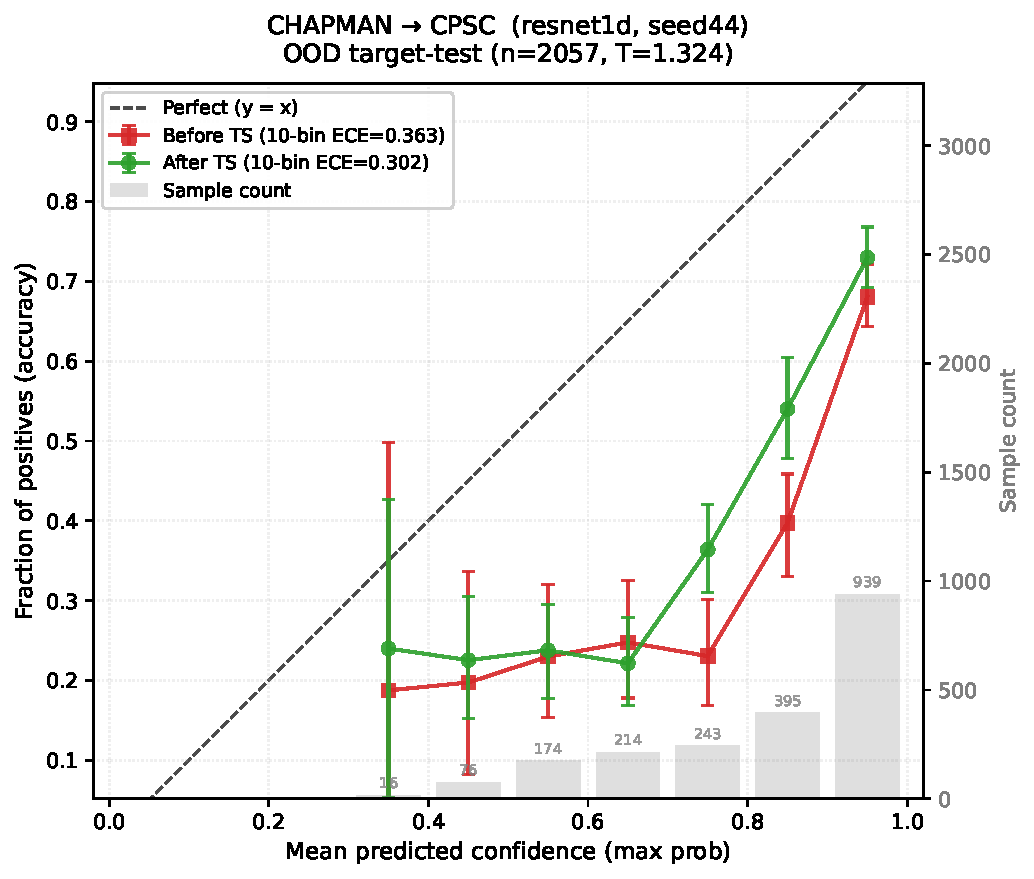
\includegraphics[width=0.32\textwidth]{figures/fig_reliability_supp_chapman_cpsc_resnet1d_seed44.pdf}
\caption{Chapman$\to$CPSC reliability diagrams: ResNet1D seeds 42--44.}
\end{figure}

\begin{figure}[h]
\centering
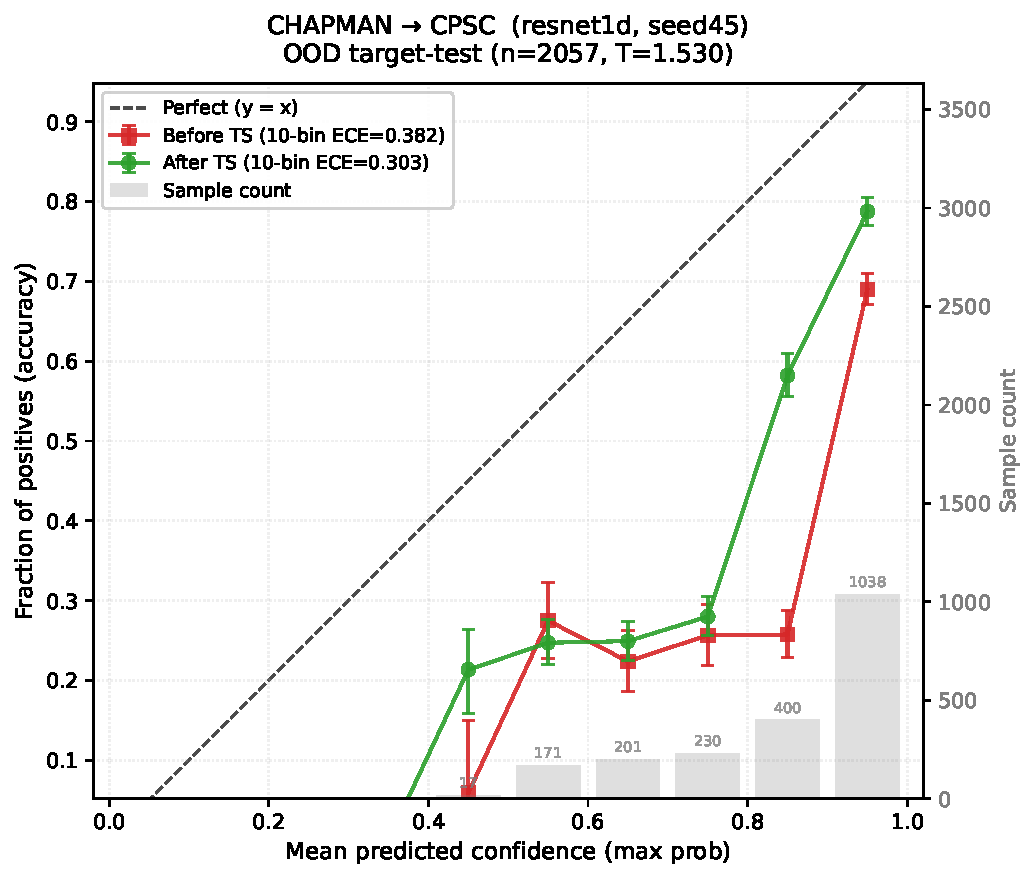
\includegraphics[width=0.45\textwidth]{figures/fig_reliability_supp_chapman_cpsc_resnet1d_seed45.pdf}
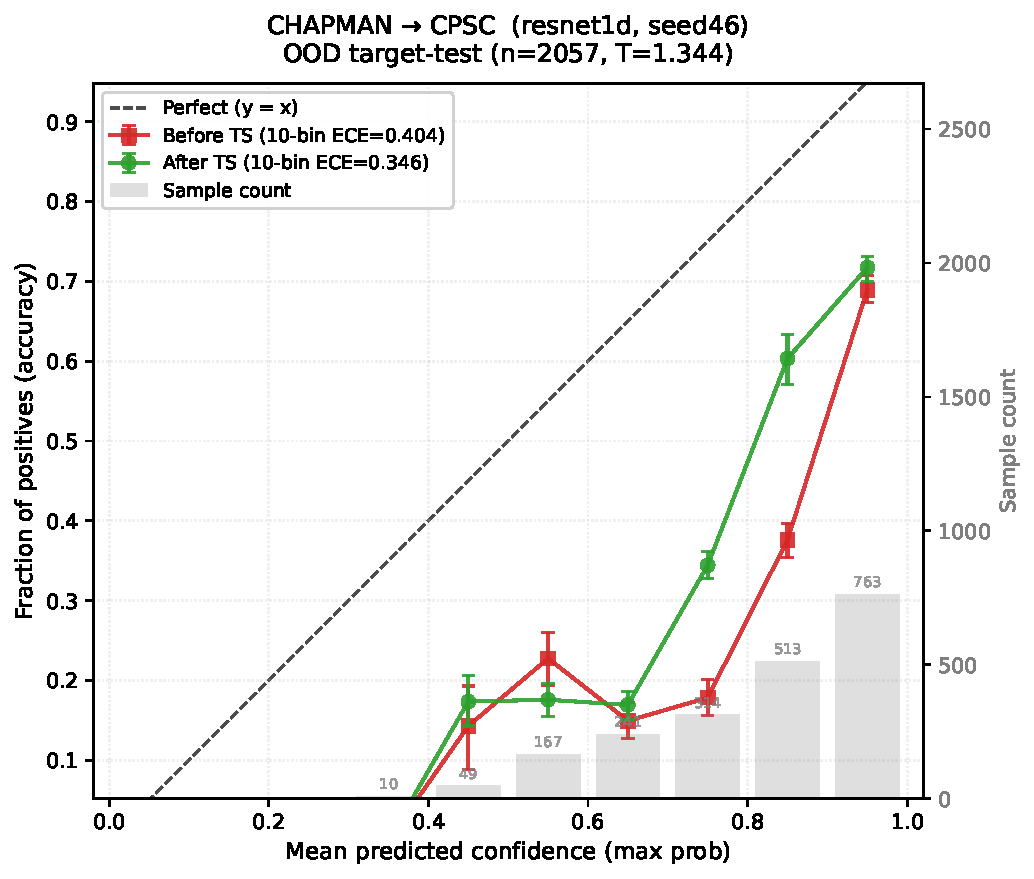
\includegraphics[width=0.45\textwidth]{figures/fig_reliability_supp_chapman_cpsc_resnet1d_seed46.pdf}
\caption{Chapman$\to$CPSC reliability diagrams: ResNet1D seeds 45--46.}
\end{figure}

\begin{figure}[h]
\centering
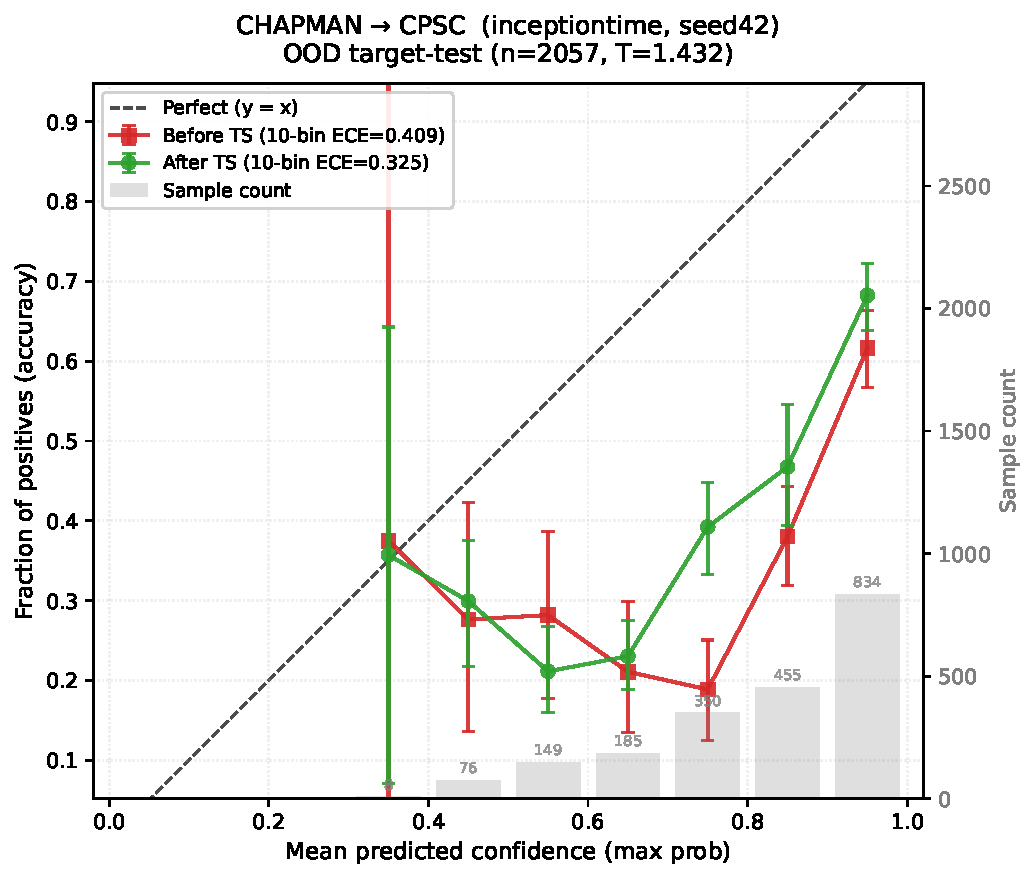
\includegraphics[width=0.32\textwidth]{figures/fig_reliability_supp_chapman_cpsc_inceptiontime_seed42.pdf}
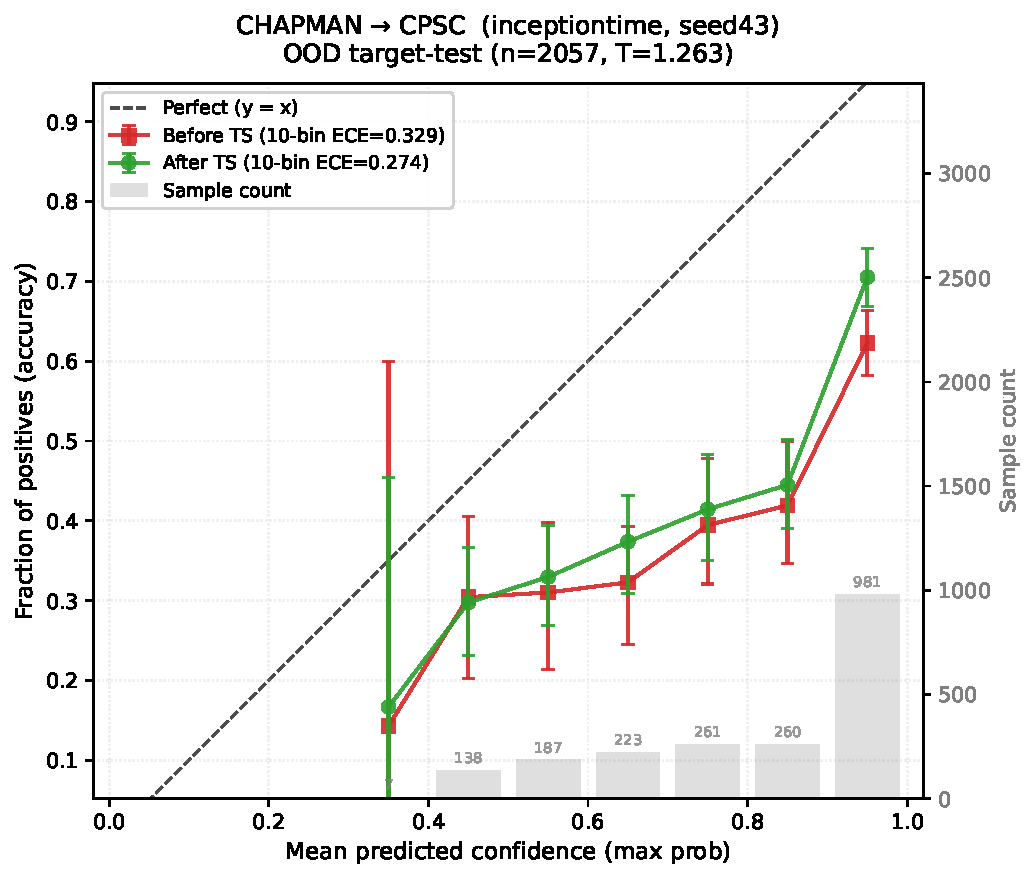
\includegraphics[width=0.32\textwidth]{figures/fig_reliability_supp_chapman_cpsc_inceptiontime_seed43.pdf}
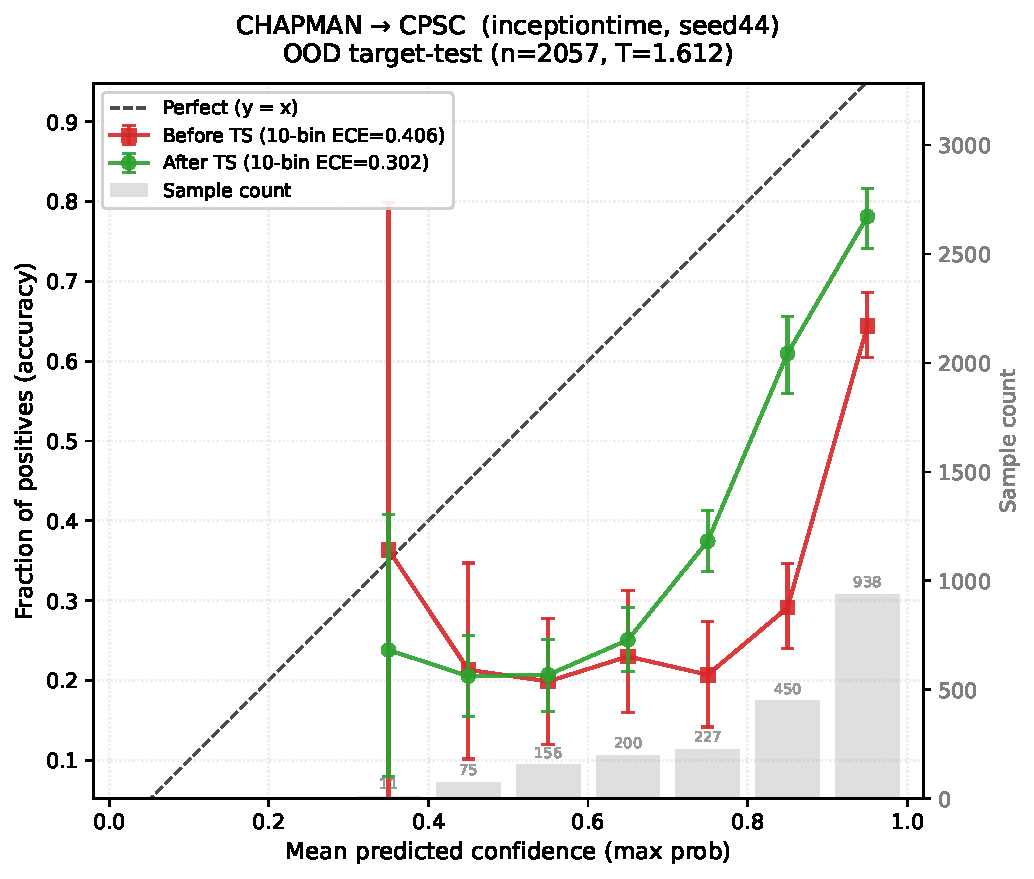
\includegraphics[width=0.32\textwidth]{figures/fig_reliability_supp_chapman_cpsc_inceptiontime_seed44.pdf}
\caption{Chapman$\to$CPSC reliability diagrams: InceptionTime seeds 42--44.}
\end{figure}

\begin{figure}[h]
\centering
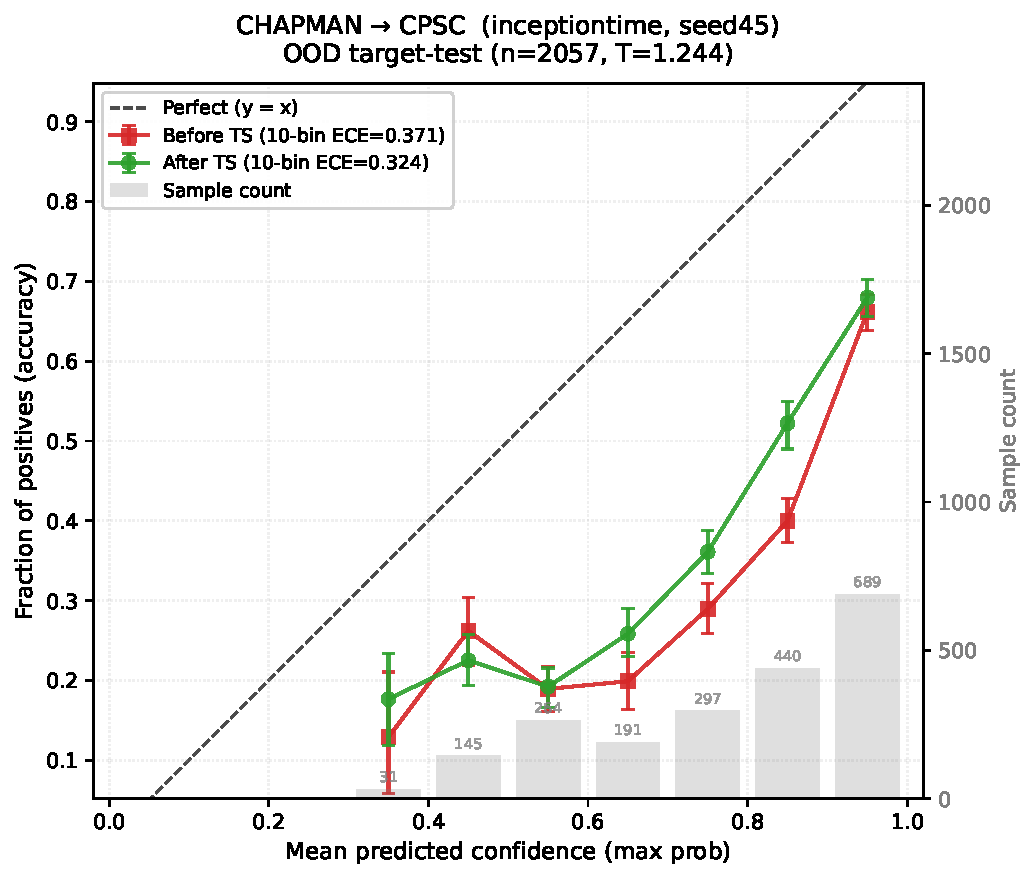
\includegraphics[width=0.45\textwidth]{figures/fig_reliability_supp_chapman_cpsc_inceptiontime_seed45.pdf}
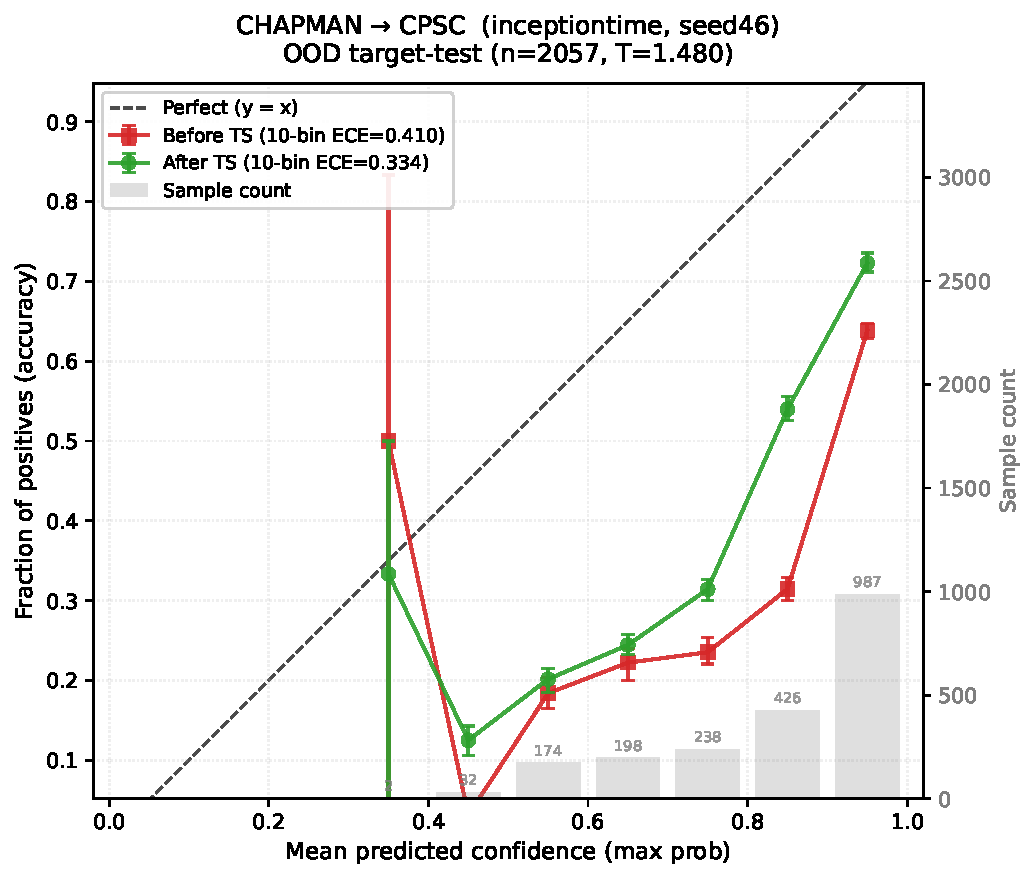
\includegraphics[width=0.45\textwidth]{figures/fig_reliability_supp_chapman_cpsc_inceptiontime_seed46.pdf}
\caption{Chapman$\to$CPSC reliability diagrams: InceptionTime seeds 45--46.}
\end{figure}

\subsubsection*{S1.2.\ Chapman$\rightarrow$PTB-XL}

\begin{figure}[h]
\centering
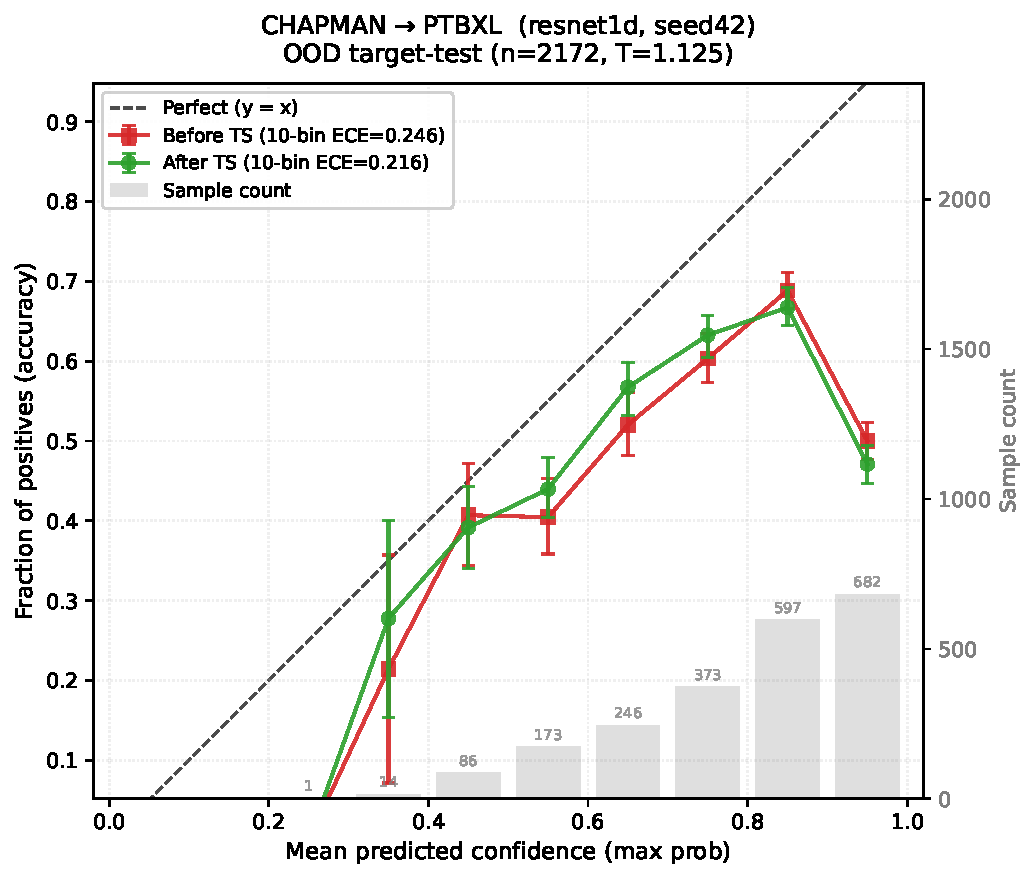
\includegraphics[width=0.32\textwidth]{figures/fig_reliability_supp_chapman_ptbxl_resnet1d_seed42.pdf}
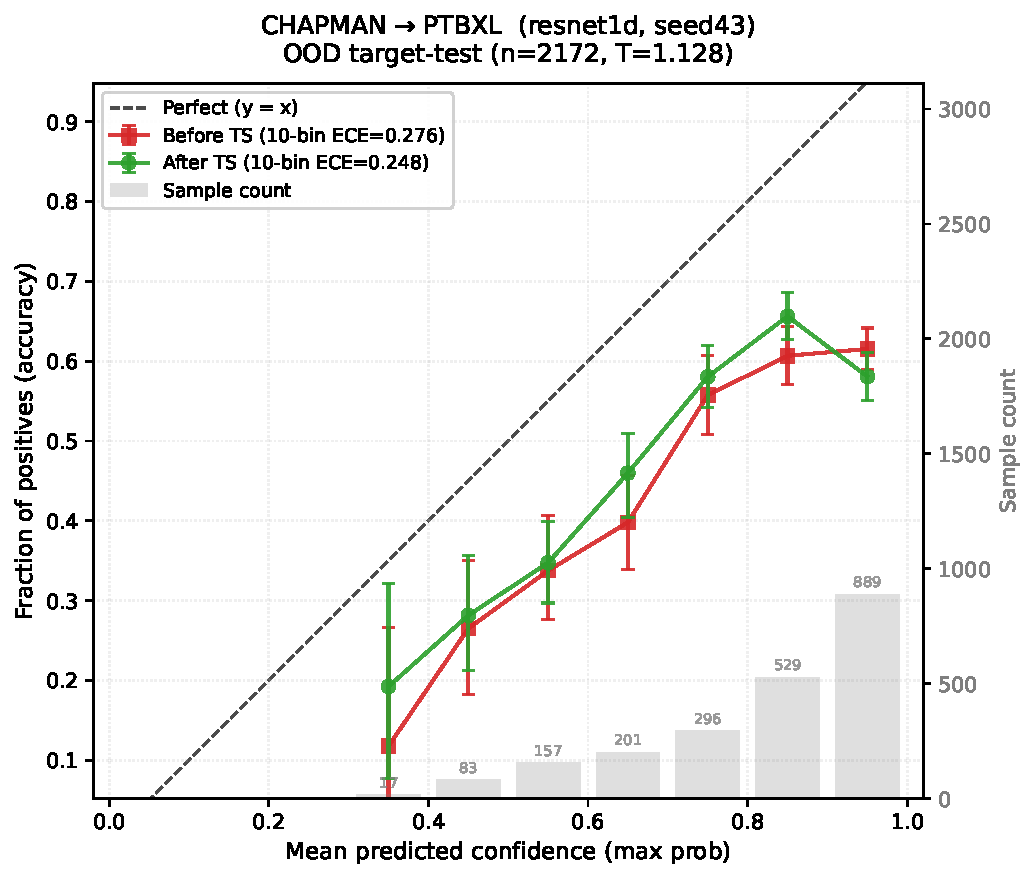
\includegraphics[width=0.32\textwidth]{figures/fig_reliability_supp_chapman_ptbxl_resnet1d_seed43.pdf}
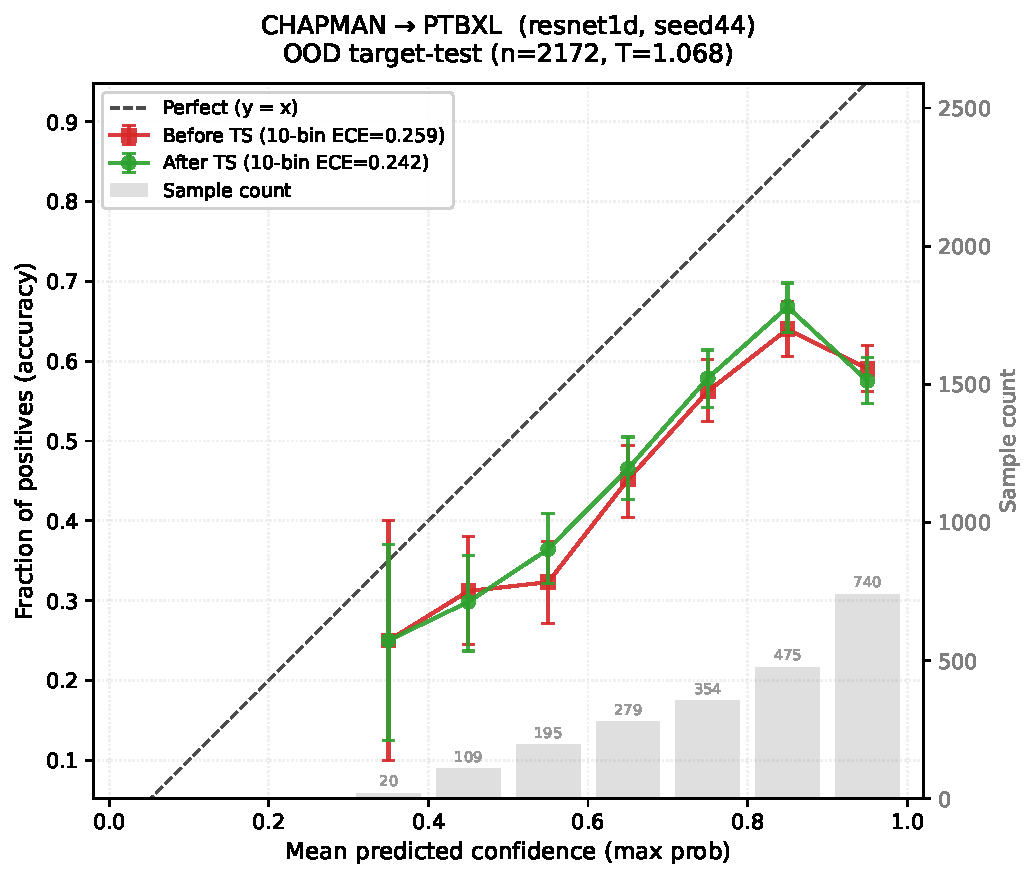
\includegraphics[width=0.32\textwidth]{figures/fig_reliability_supp_chapman_ptbxl_resnet1d_seed44.pdf}
\caption{Chapman$\to$PTB-XL reliability diagrams: ResNet1D seeds 42--44.}
\end{figure}

\begin{figure}[h]
\centering
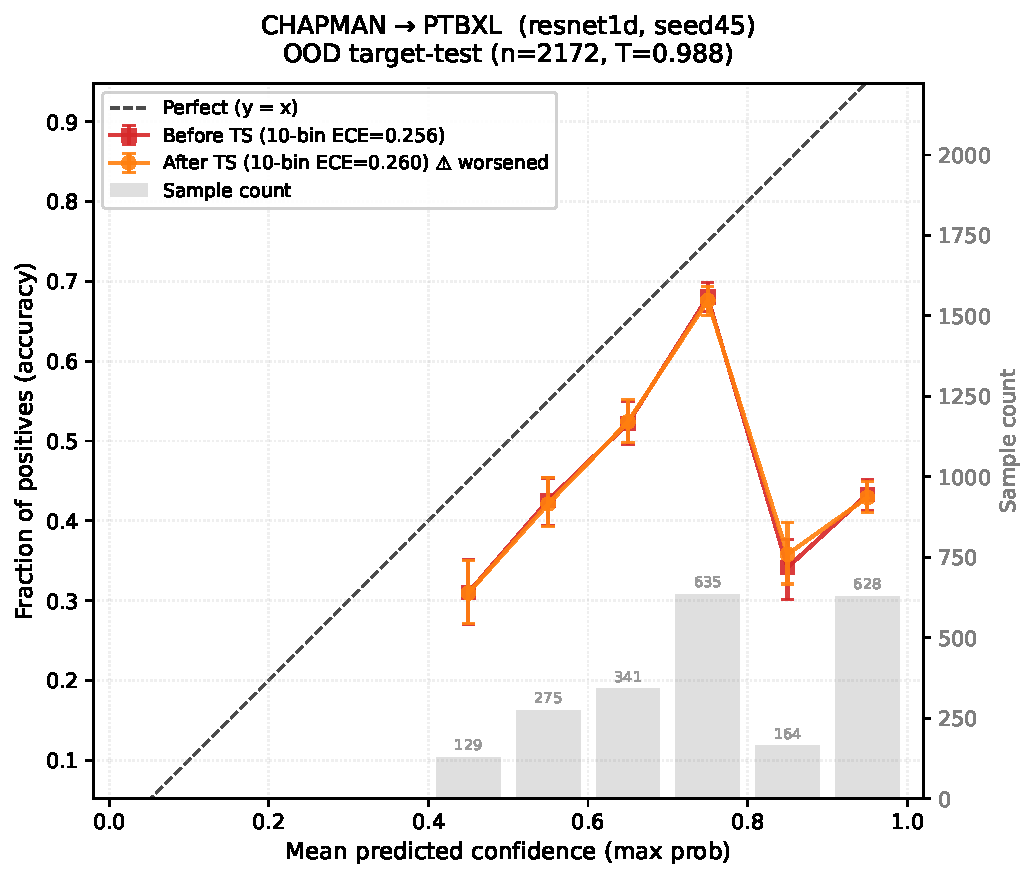
\includegraphics[width=0.45\textwidth]{figures/fig_reliability_supp_chapman_ptbxl_resnet1d_seed45.pdf}
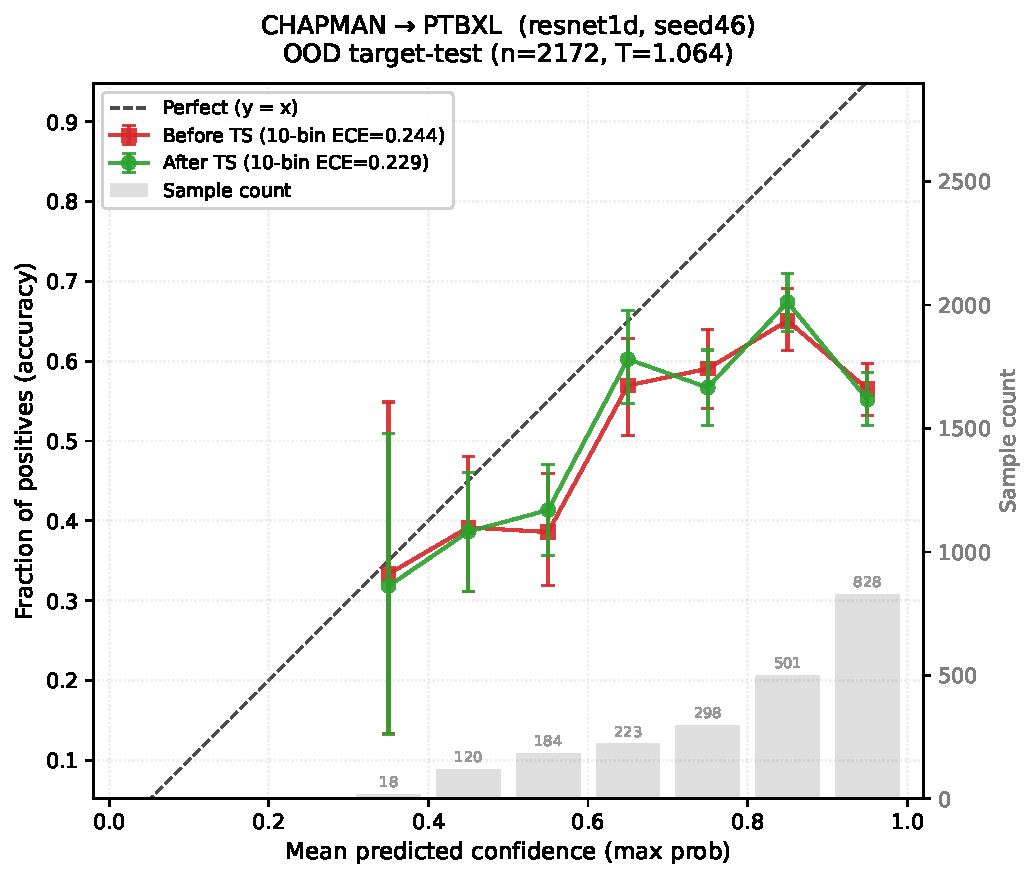
\includegraphics[width=0.45\textwidth]{figures/fig_reliability_supp_chapman_ptbxl_resnet1d_seed46.pdf}
\caption{Chapman$\to$PTB-XL reliability diagrams: ResNet1D seeds 45--46.}
\end{figure}

\begin{figure}[h]
\centering
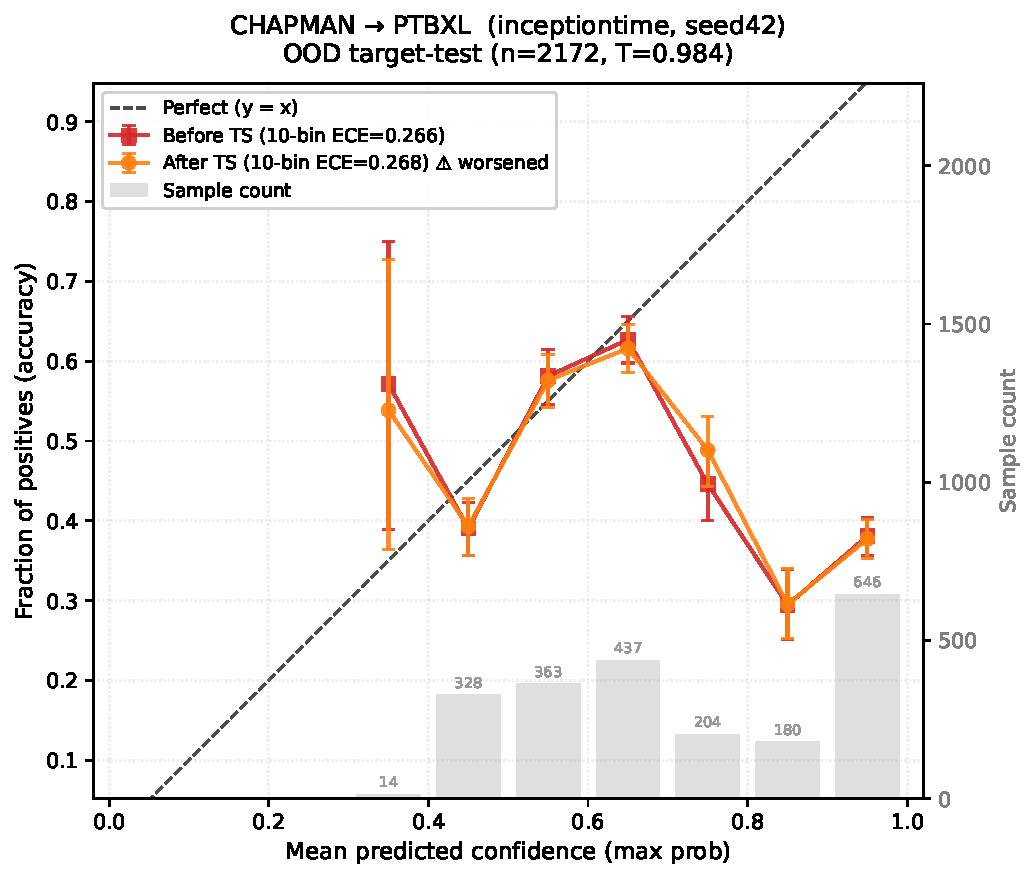
\includegraphics[width=0.32\textwidth]{figures/fig_reliability_supp_chapman_ptbxl_inceptiontime_seed42.pdf}
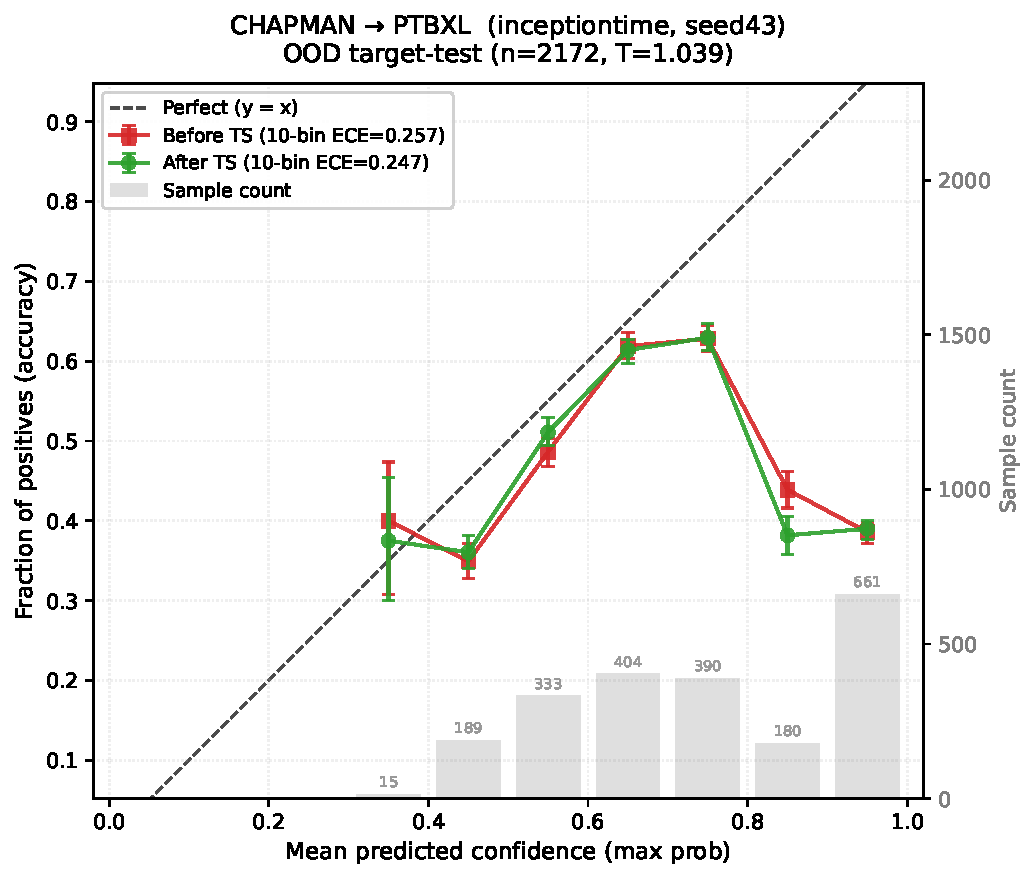
\includegraphics[width=0.32\textwidth]{figures/fig_reliability_supp_chapman_ptbxl_inceptiontime_seed43.pdf}
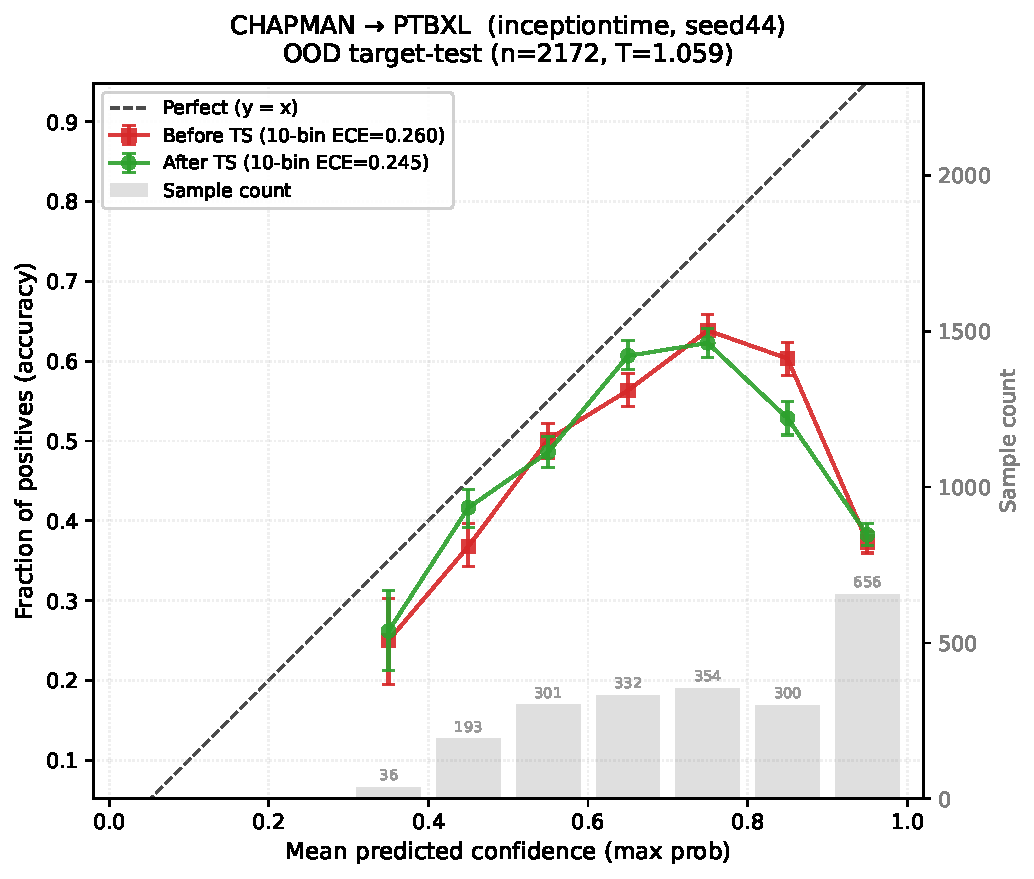
\includegraphics[width=0.32\textwidth]{figures/fig_reliability_supp_chapman_ptbxl_inceptiontime_seed44.pdf}
\caption{Chapman$\to$PTB-XL reliability diagrams: InceptionTime seeds 42--44.}
\end{figure}

\begin{figure}[h]
\centering
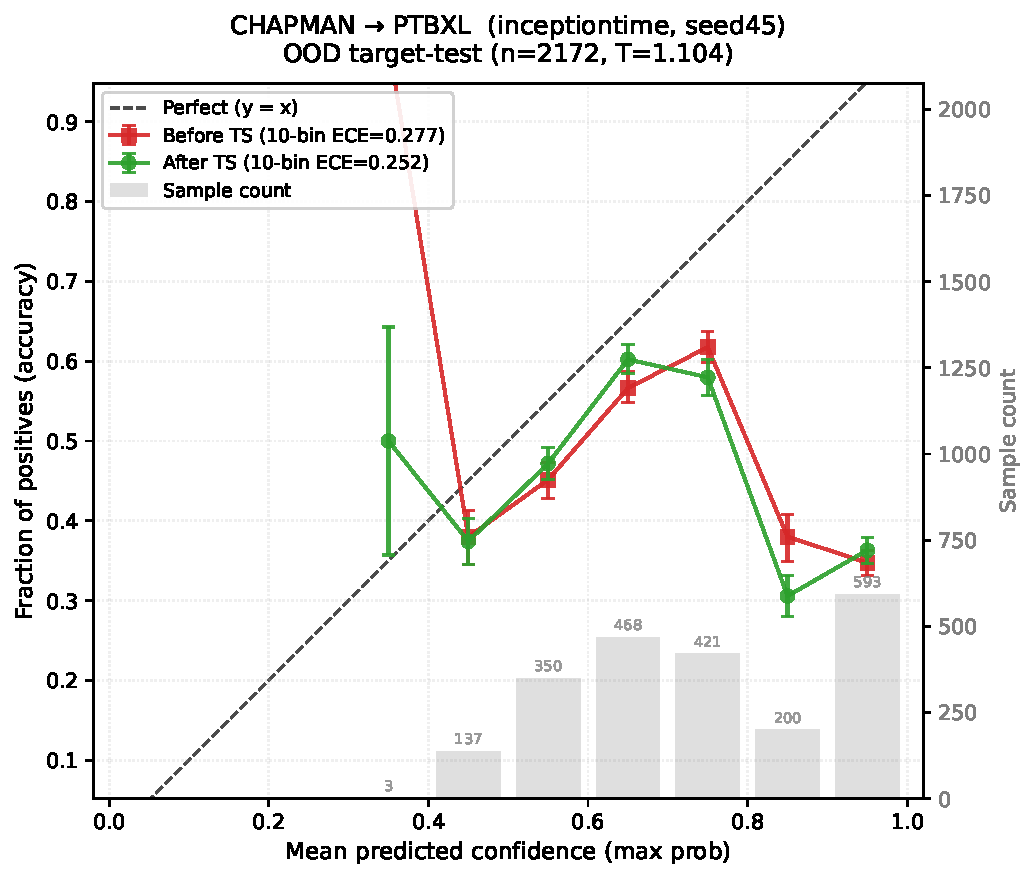
\includegraphics[width=0.45\textwidth]{figures/fig_reliability_supp_chapman_ptbxl_inceptiontime_seed45.pdf}
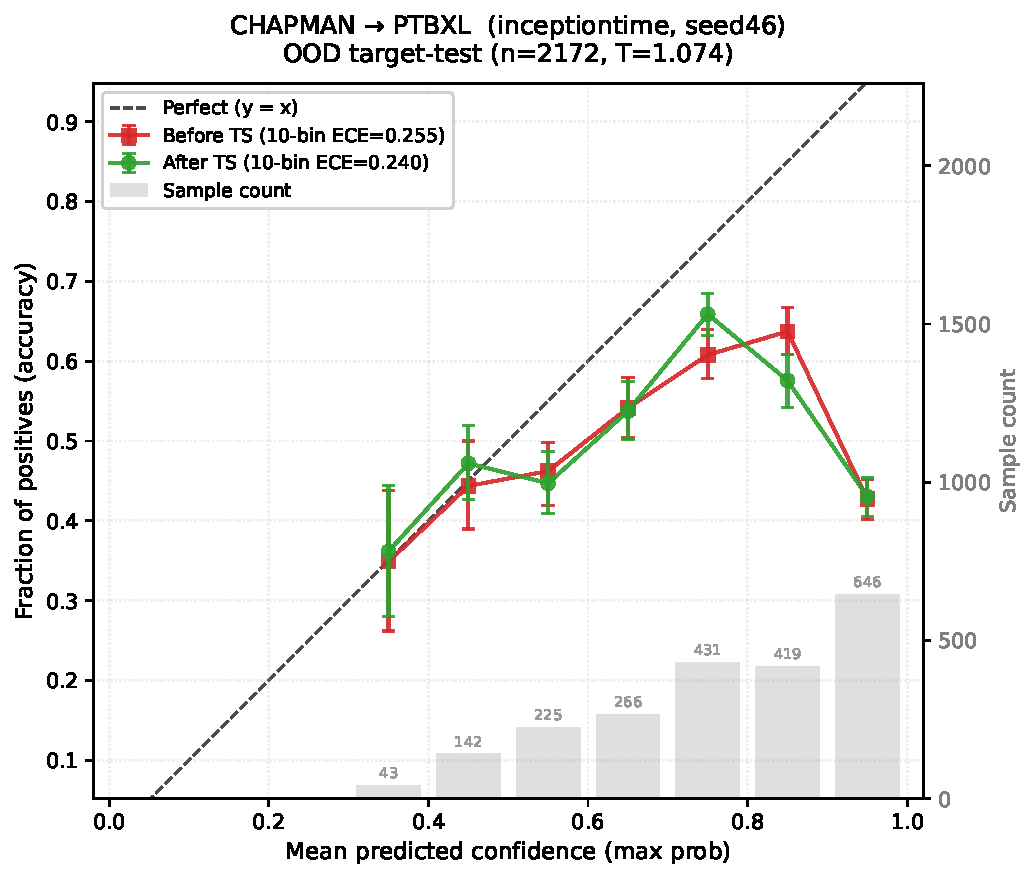
\includegraphics[width=0.45\textwidth]{figures/fig_reliability_supp_chapman_ptbxl_inceptiontime_seed46.pdf}
\caption{Chapman$\to$PTB-XL reliability diagrams: InceptionTime seeds 45--46.}
\end{figure}

\subsubsection*{S1.3.\ CPSC$\rightarrow$Chapman}

\begin{figure}[h]
\centering
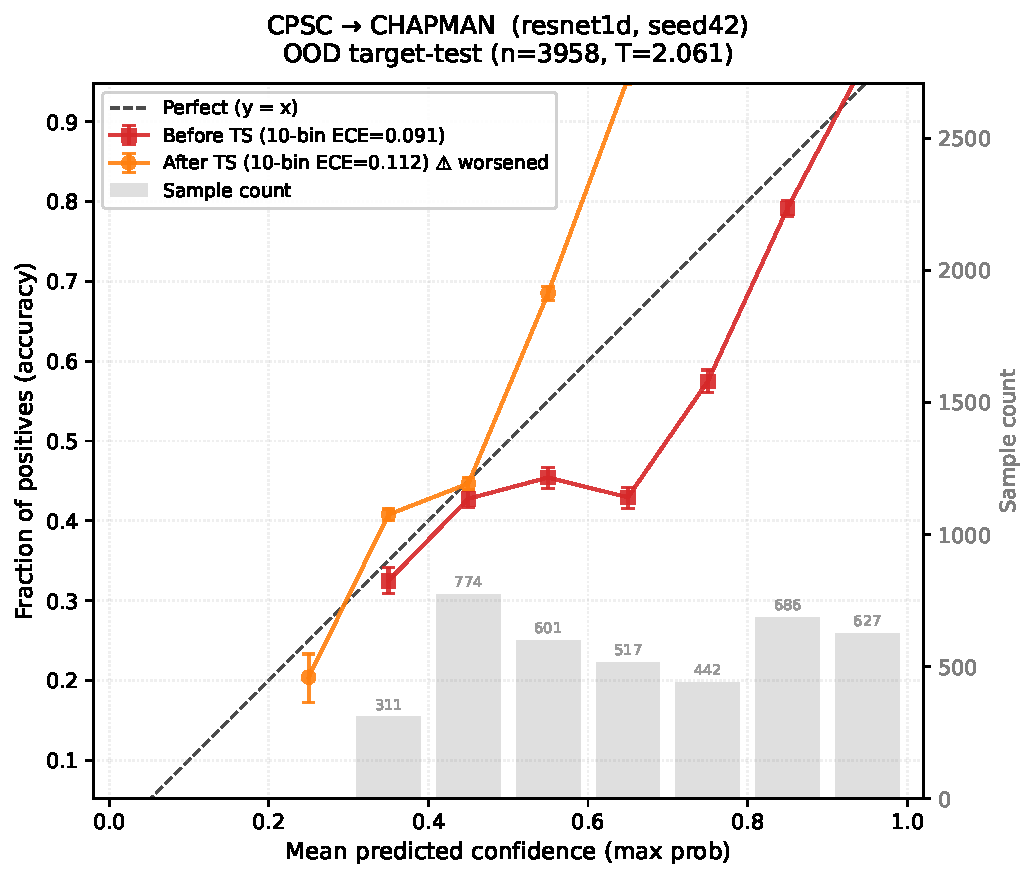
\includegraphics[width=0.32\textwidth]{figures/fig_reliability_supp_cpsc_chapman_resnet1d_seed42.pdf}
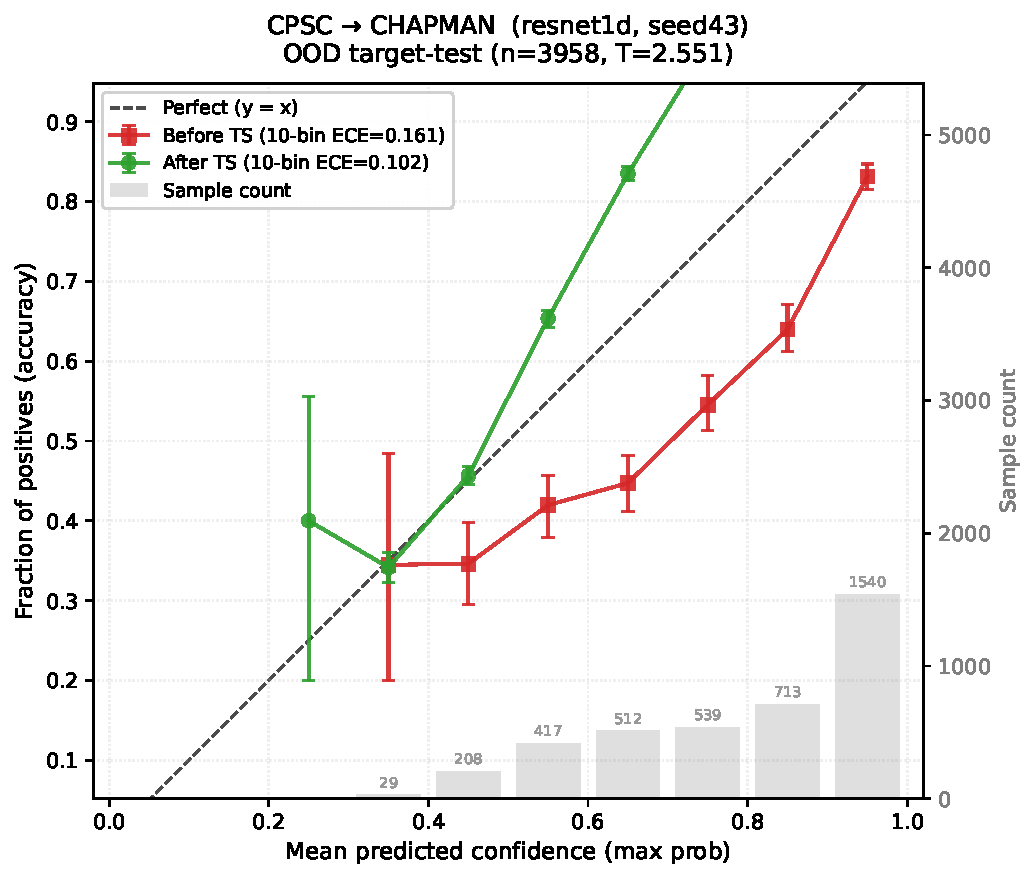
\includegraphics[width=0.32\textwidth]{figures/fig_reliability_supp_cpsc_chapman_resnet1d_seed43.pdf}
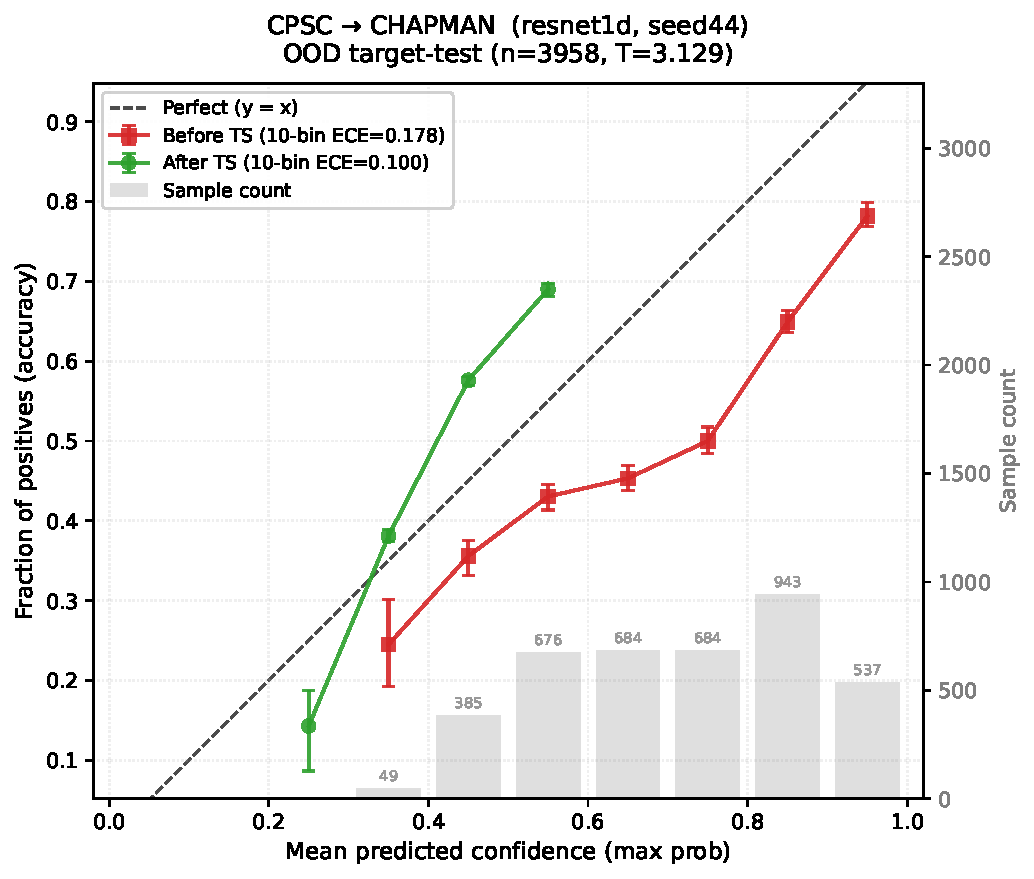
\includegraphics[width=0.32\textwidth]{figures/fig_reliability_supp_cpsc_chapman_resnet1d_seed44.pdf}
\caption{CPSC$\to$Chapman reliability diagrams: ResNet1D seeds 42--44.}
\end{figure}

\begin{figure}[h]
\centering
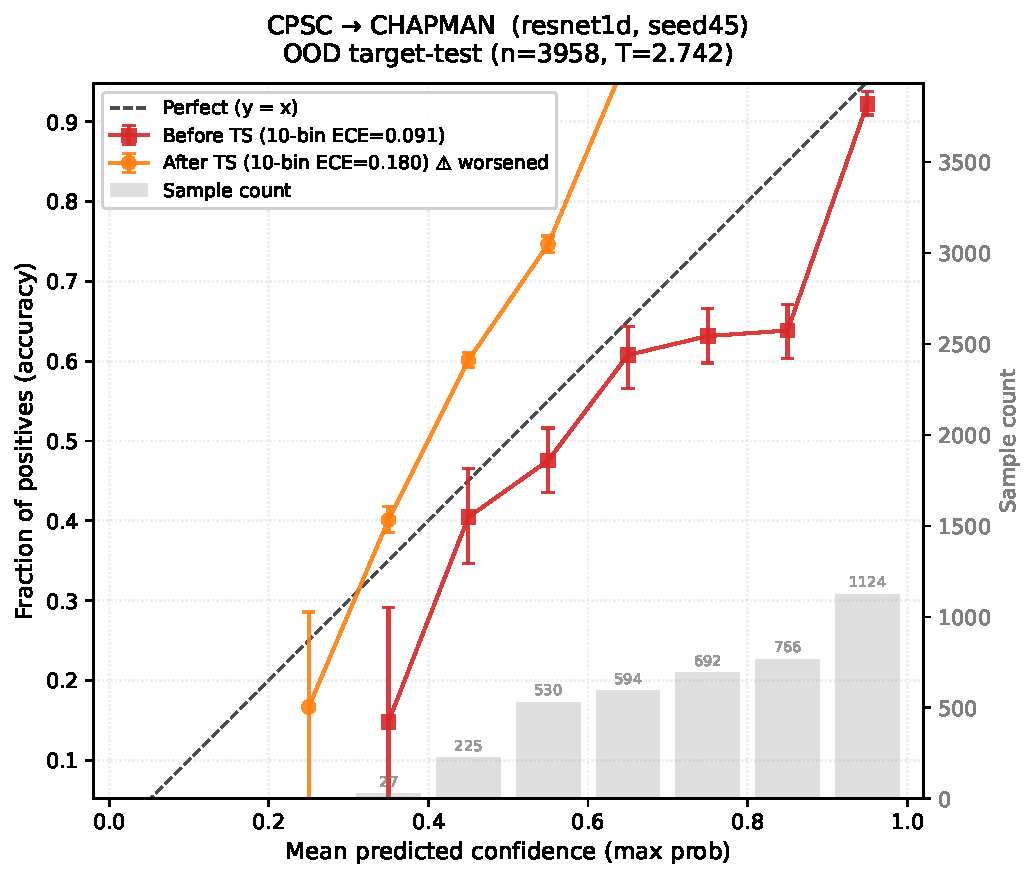
\includegraphics[width=0.45\textwidth]{figures/fig_reliability_supp_cpsc_chapman_resnet1d_seed45.pdf}
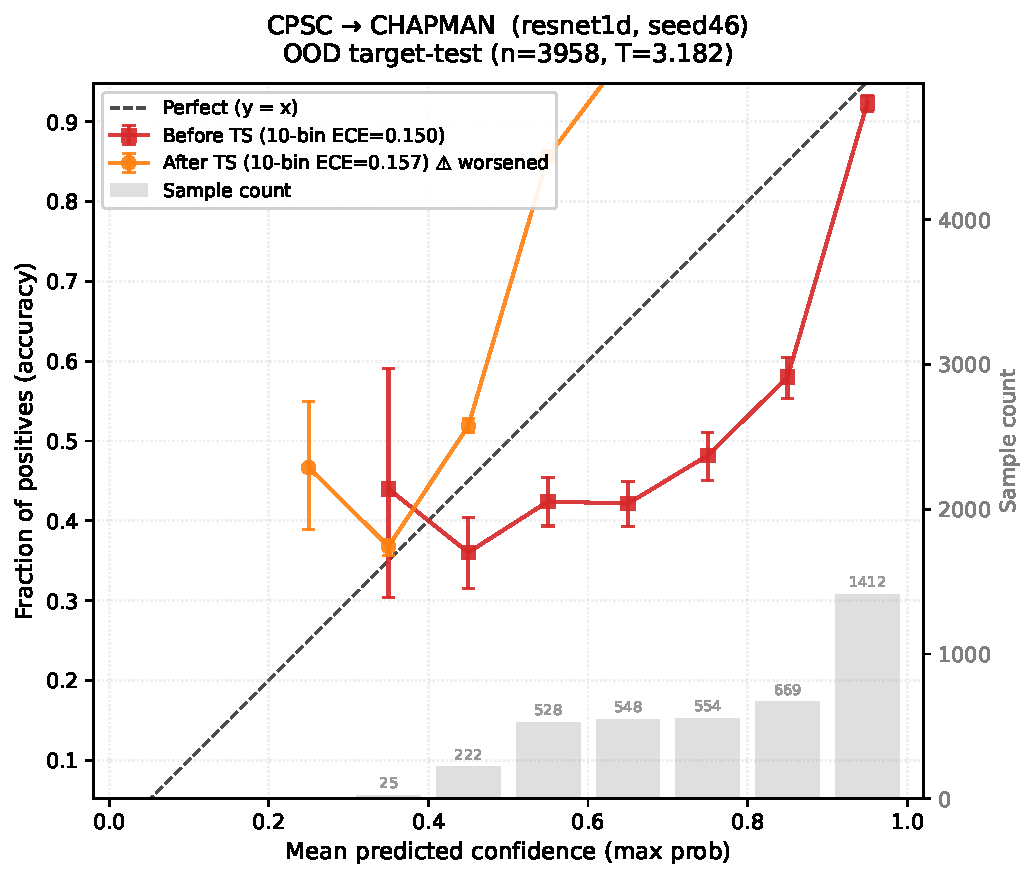
\includegraphics[width=0.45\textwidth]{figures/fig_reliability_supp_cpsc_chapman_resnet1d_seed46.pdf}
\caption{CPSC$\to$Chapman reliability diagrams: ResNet1D seeds 45--46.}
\end{figure}

\begin{figure}[h]
\centering
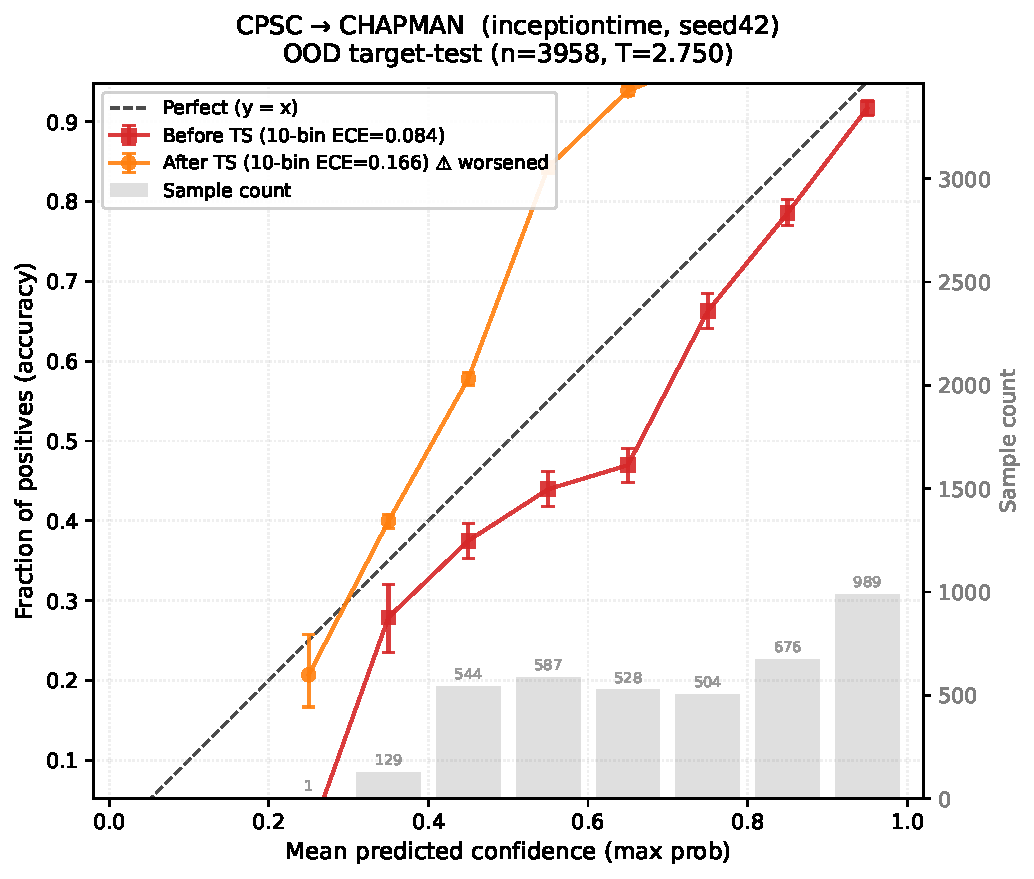
\includegraphics[width=0.32\textwidth]{figures/fig_reliability_supp_cpsc_chapman_inceptiontime_seed42.pdf}
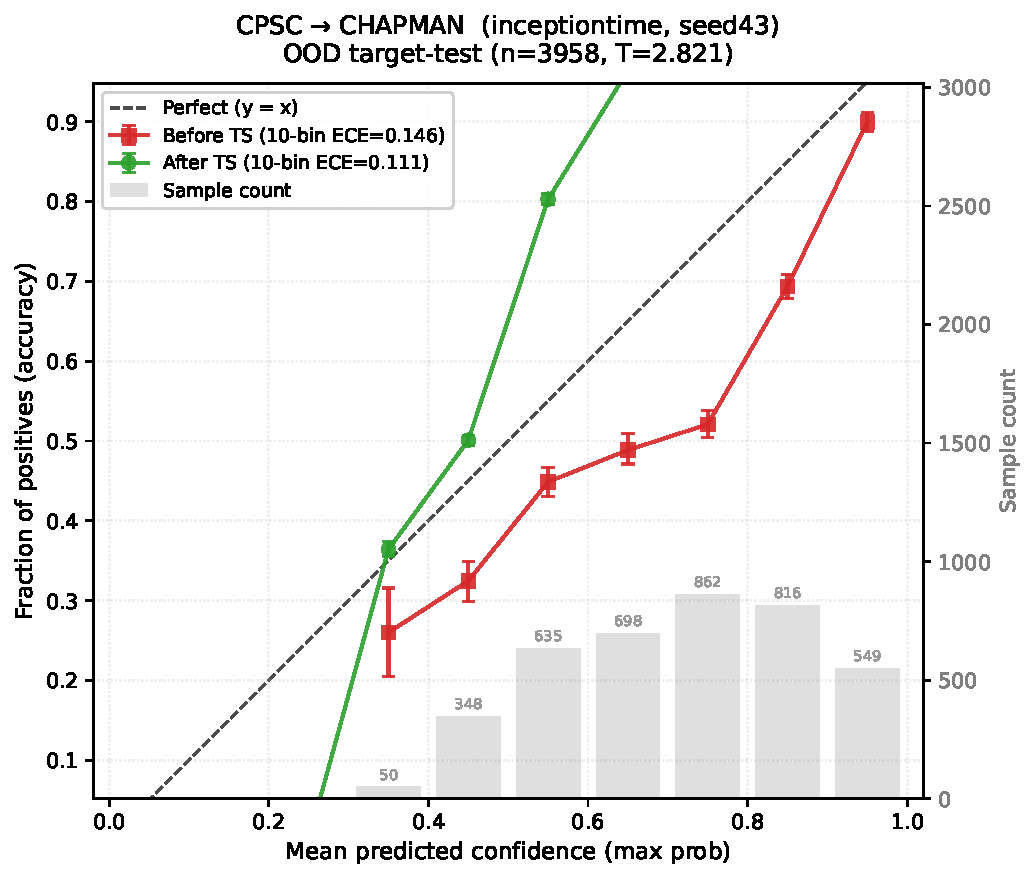
\includegraphics[width=0.32\textwidth]{figures/fig_reliability_supp_cpsc_chapman_inceptiontime_seed43.pdf}
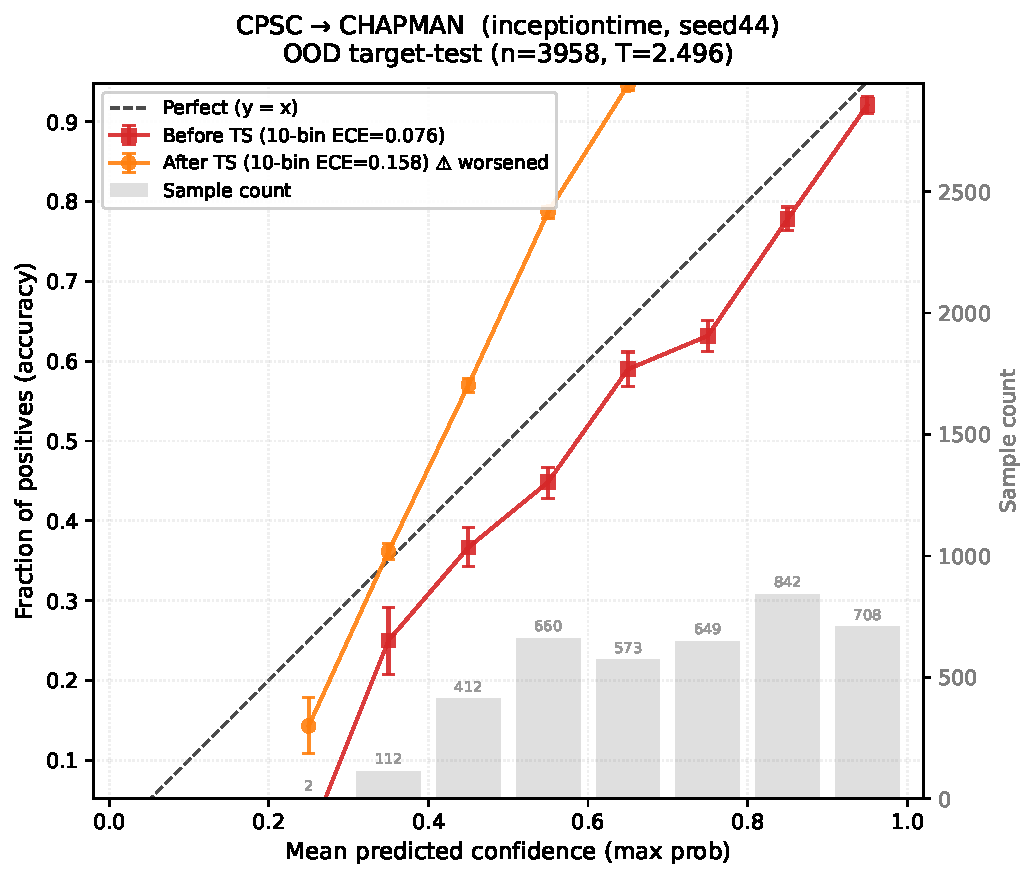
\includegraphics[width=0.32\textwidth]{figures/fig_reliability_supp_cpsc_chapman_inceptiontime_seed44.pdf}
\caption{CPSC$\to$Chapman reliability diagrams: InceptionTime seeds 42--44.}
\end{figure}

\begin{figure}[h]
\centering
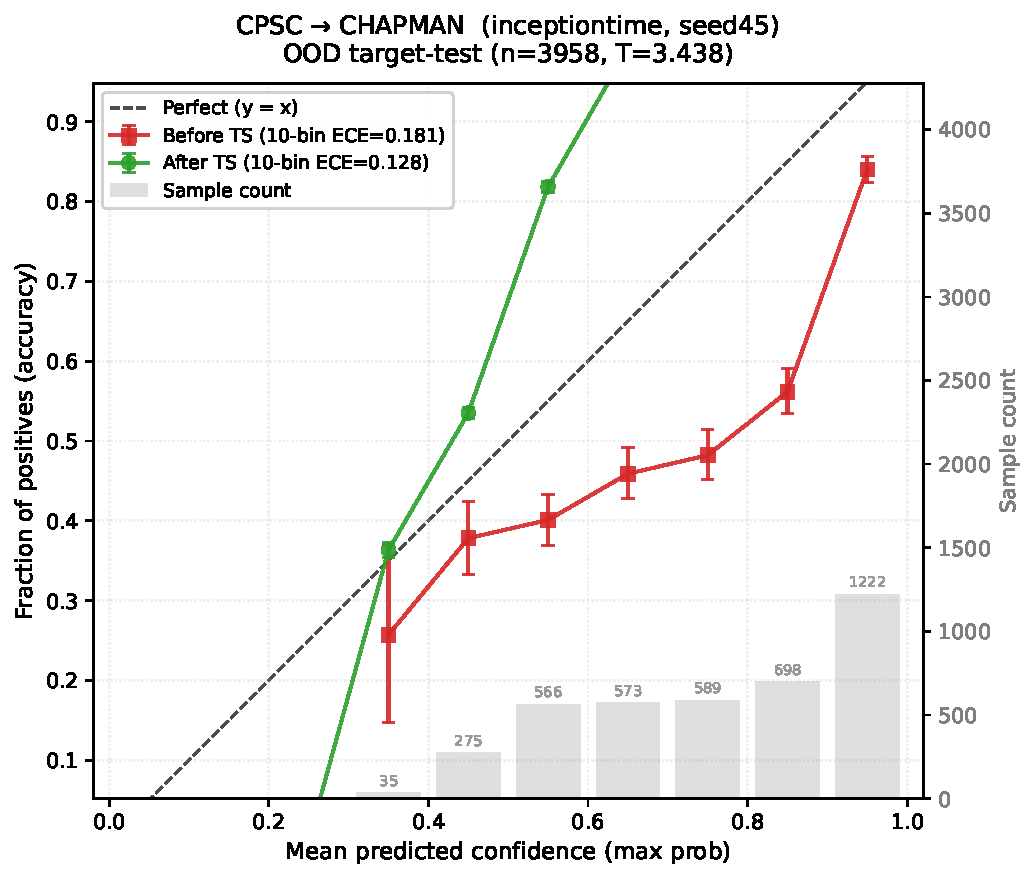
\includegraphics[width=0.45\textwidth]{figures/fig_reliability_supp_cpsc_chapman_inceptiontime_seed45.pdf}
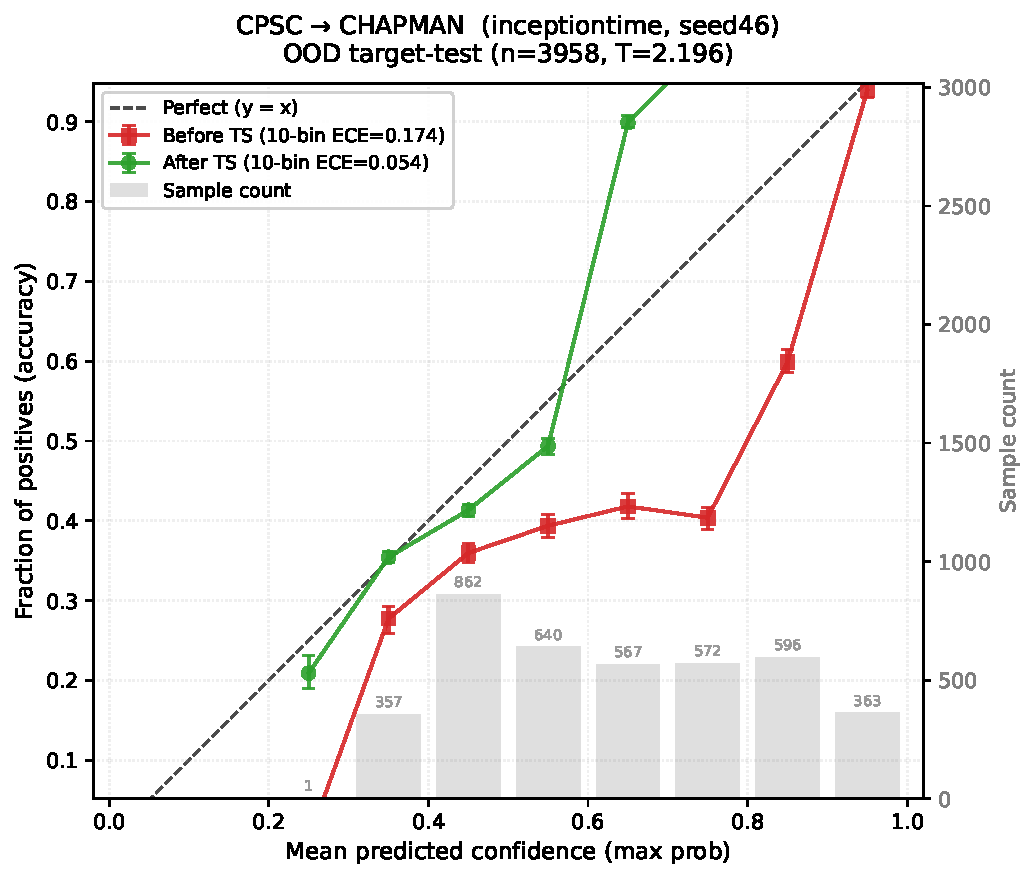
\includegraphics[width=0.45\textwidth]{figures/fig_reliability_supp_cpsc_chapman_inceptiontime_seed46.pdf}
\caption{CPSC$\to$Chapman reliability diagrams: InceptionTime seeds 45--46.}
\end{figure}

\subsubsection*{S1.4.\ CPSC$\rightarrow$PTB-XL}

\begin{figure}[h]
\centering
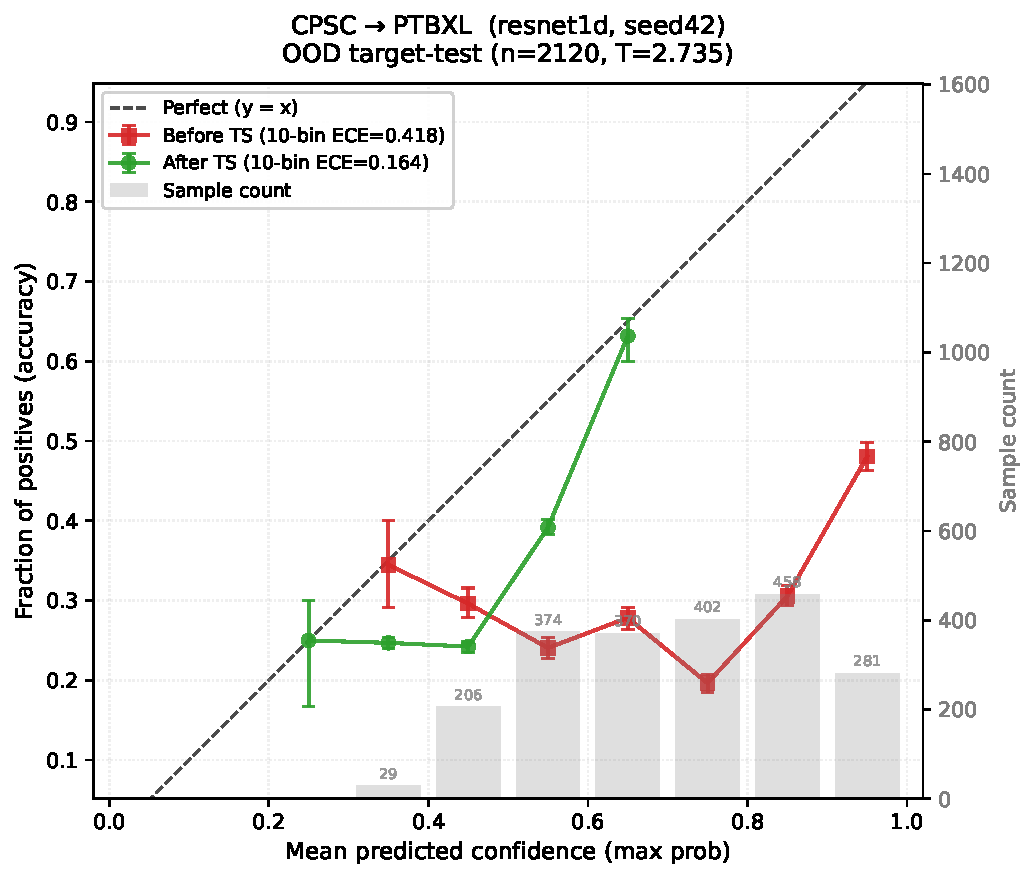
\includegraphics[width=0.32\textwidth]{figures/fig_reliability_supp_cpsc_ptbxl_resnet1d_seed42.pdf}
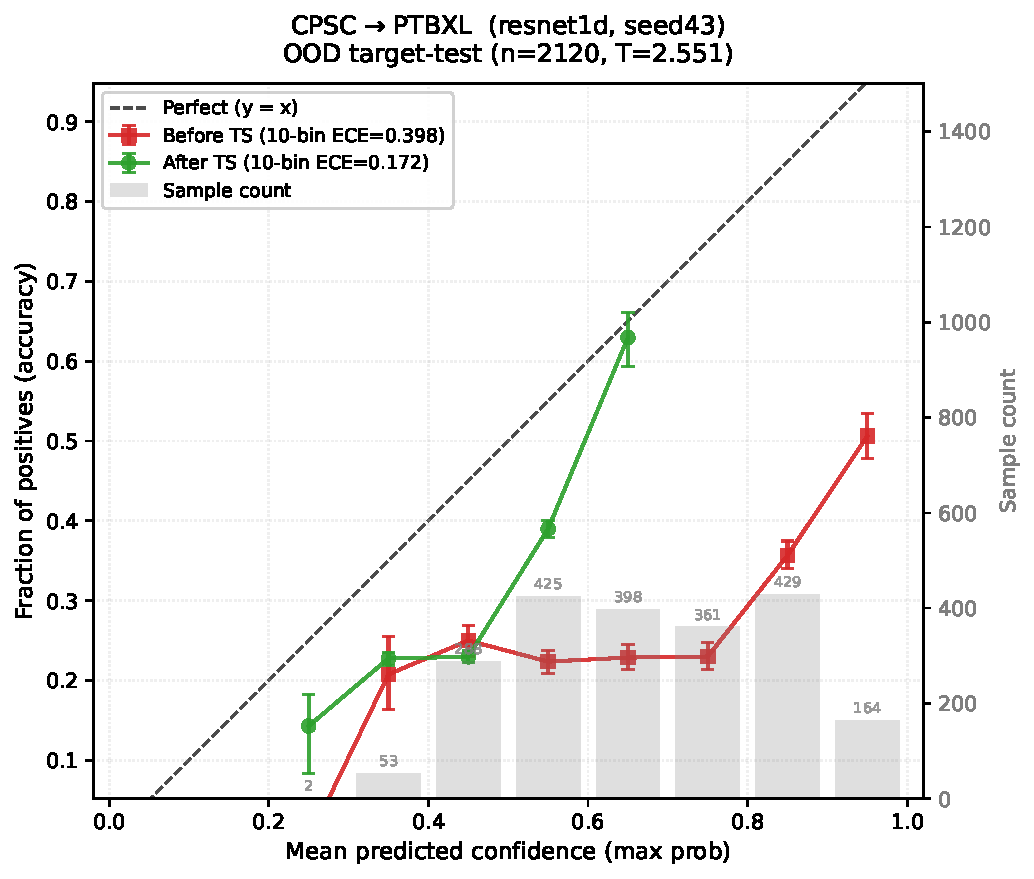
\includegraphics[width=0.32\textwidth]{figures/fig_reliability_supp_cpsc_ptbxl_resnet1d_seed43.pdf}
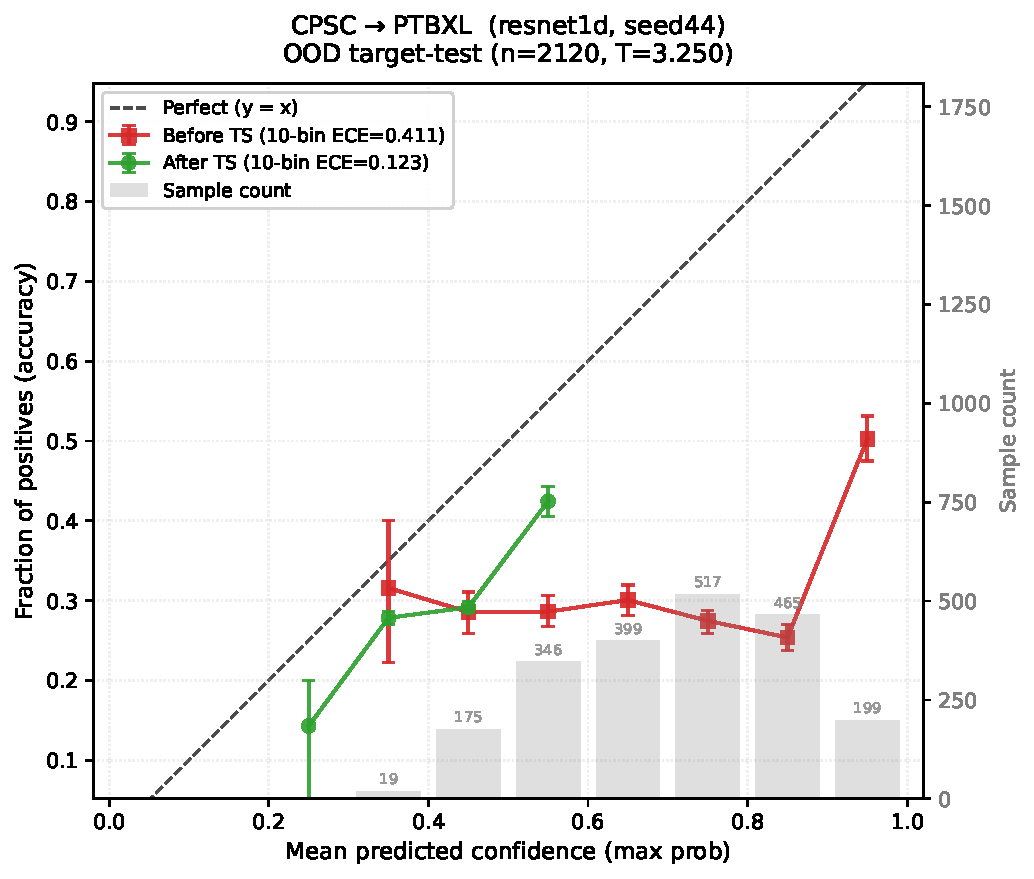
\includegraphics[width=0.32\textwidth]{figures/fig_reliability_supp_cpsc_ptbxl_resnet1d_seed44.pdf}
\caption{CPSC$\to$PTB-XL reliability diagrams: ResNet1D seeds 42--44.}
\end{figure}

\begin{figure}[h]
\centering
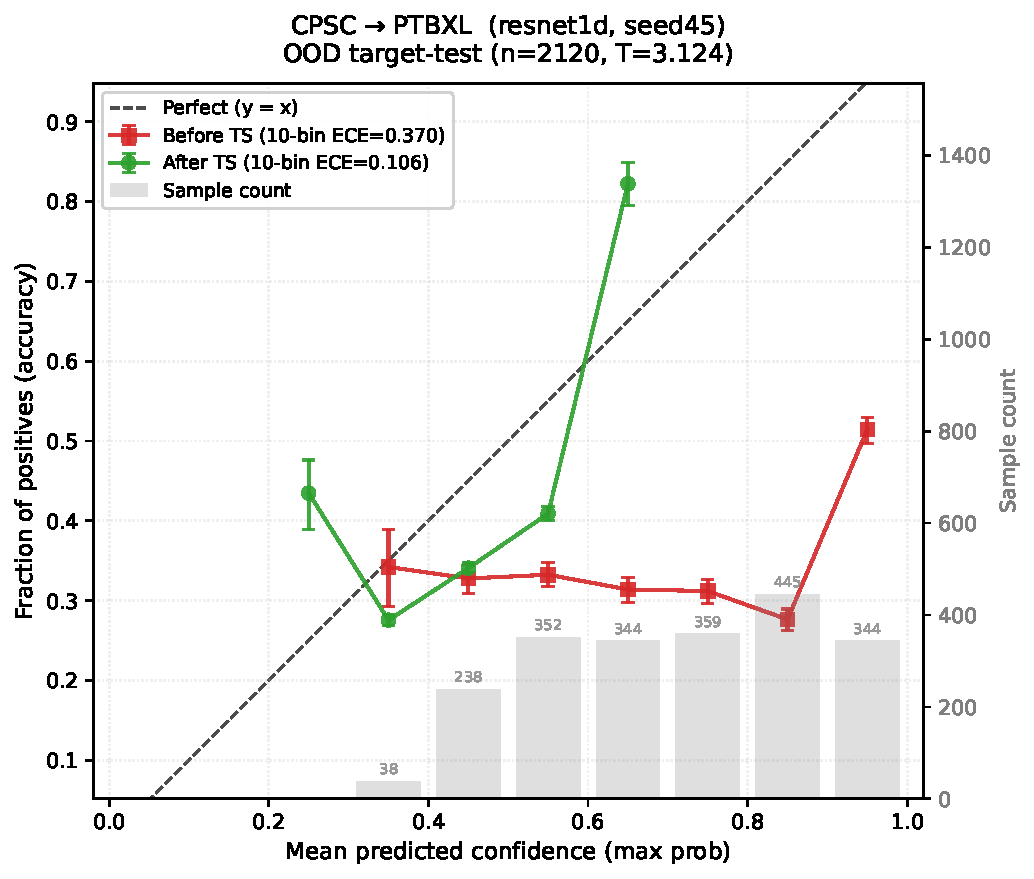
\includegraphics[width=0.45\textwidth]{figures/fig_reliability_supp_cpsc_ptbxl_resnet1d_seed45.pdf}
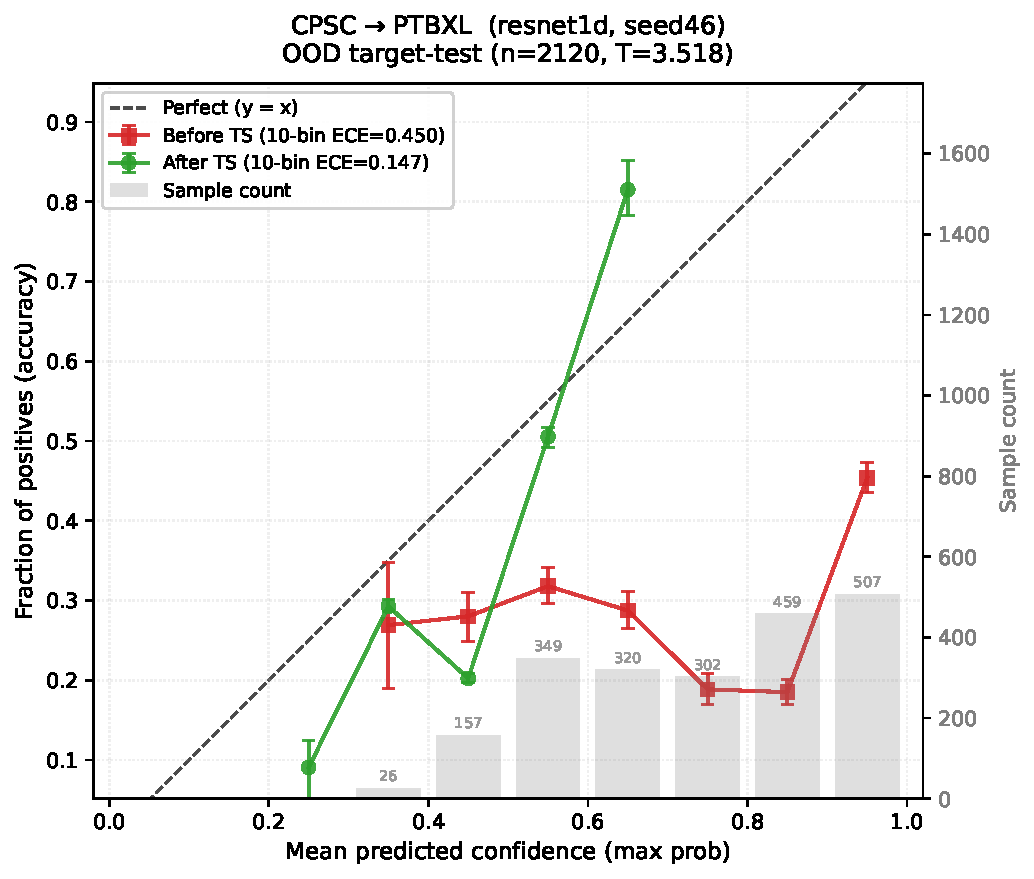
\includegraphics[width=0.45\textwidth]{figures/fig_reliability_supp_cpsc_ptbxl_resnet1d_seed46.pdf}
\caption{CPSC$\to$PTB-XL reliability diagrams: ResNet1D seeds 45--46.}
\end{figure}

\begin{figure}[h]
\centering
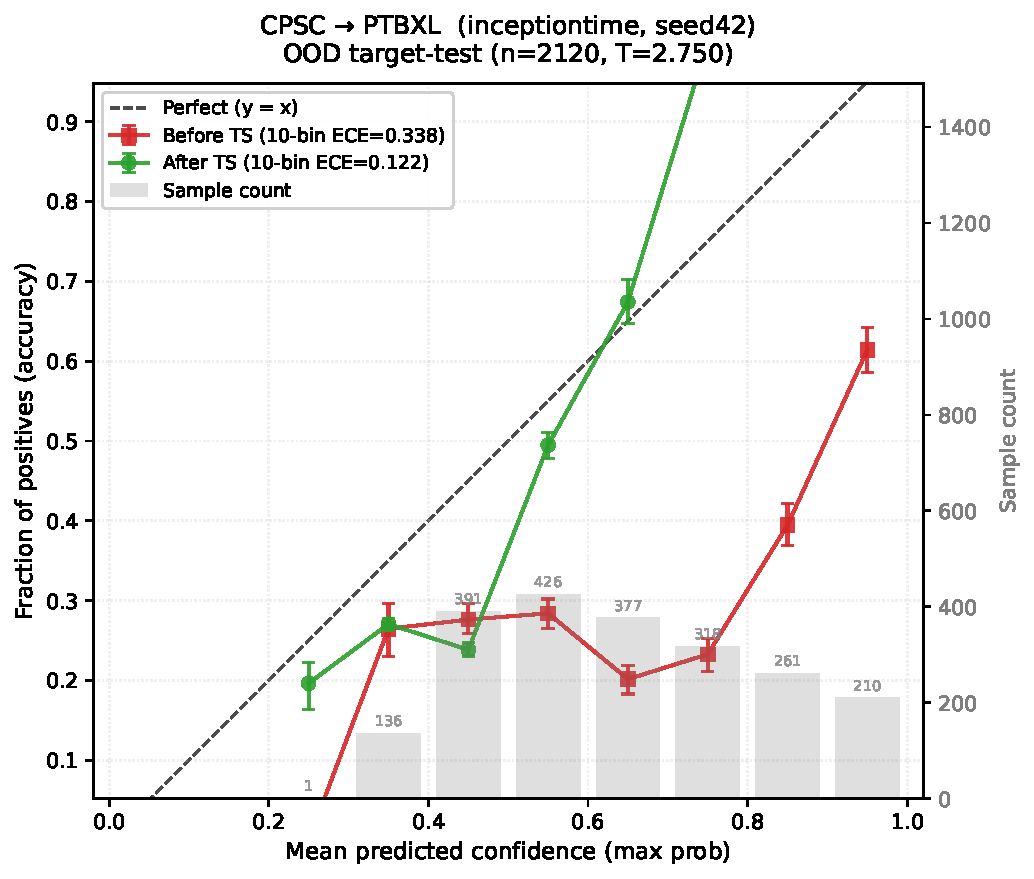
\includegraphics[width=0.32\textwidth]{figures/fig_reliability_supp_cpsc_ptbxl_inceptiontime_seed42.pdf}
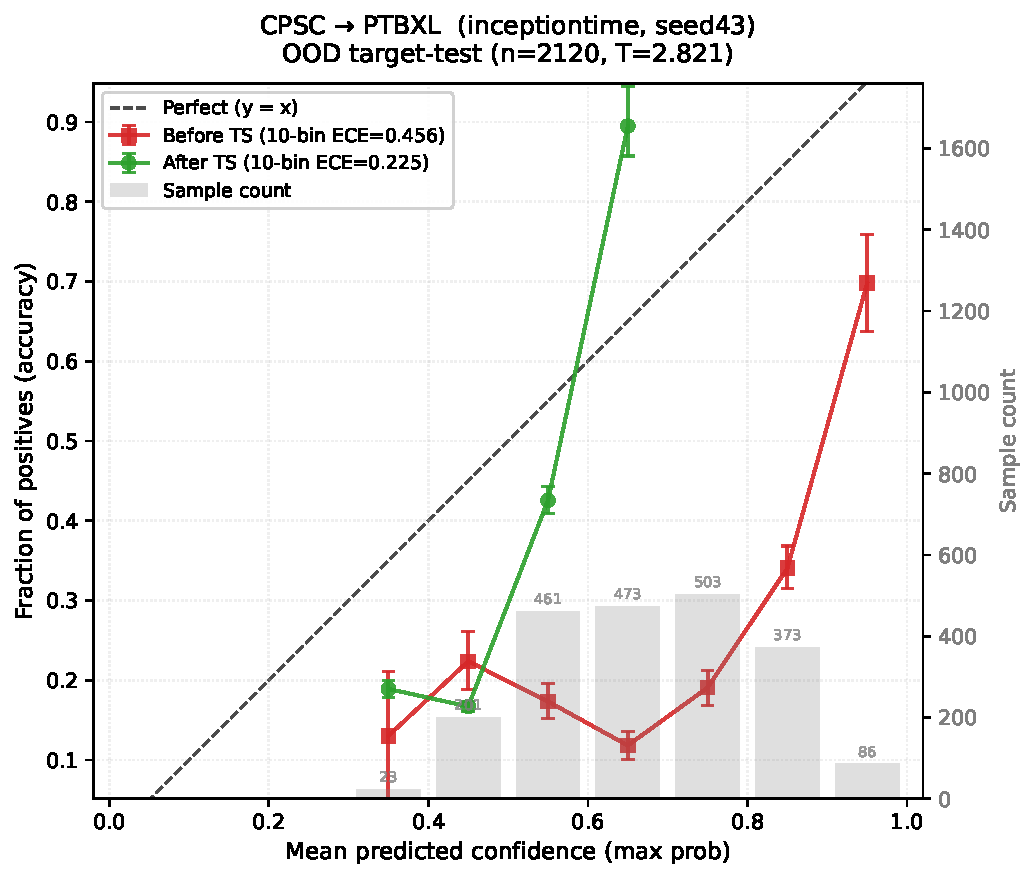
\includegraphics[width=0.32\textwidth]{figures/fig_reliability_supp_cpsc_ptbxl_inceptiontime_seed43.pdf}
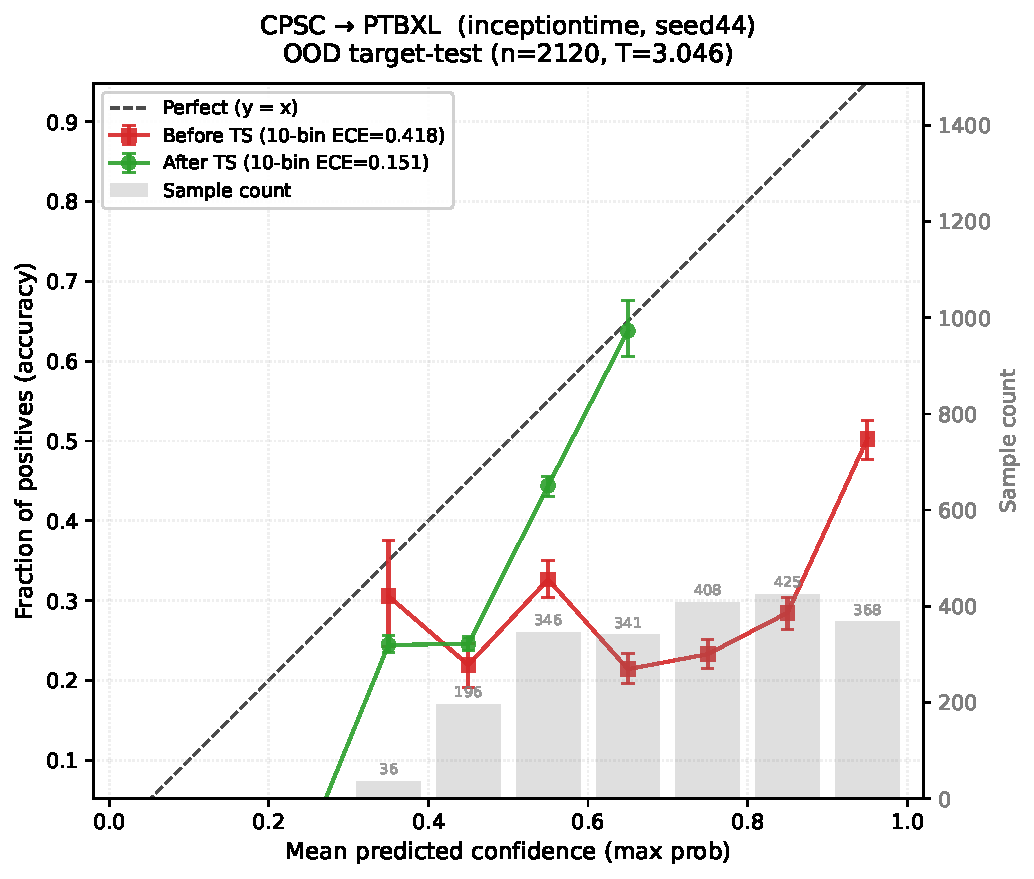
\includegraphics[width=0.32\textwidth]{figures/fig_reliability_supp_cpsc_ptbxl_inceptiontime_seed44.pdf}
\caption{CPSC$\to$PTB-XL reliability diagrams: InceptionTime seeds 42--44.}
\end{figure}

\begin{figure}[h]
\centering
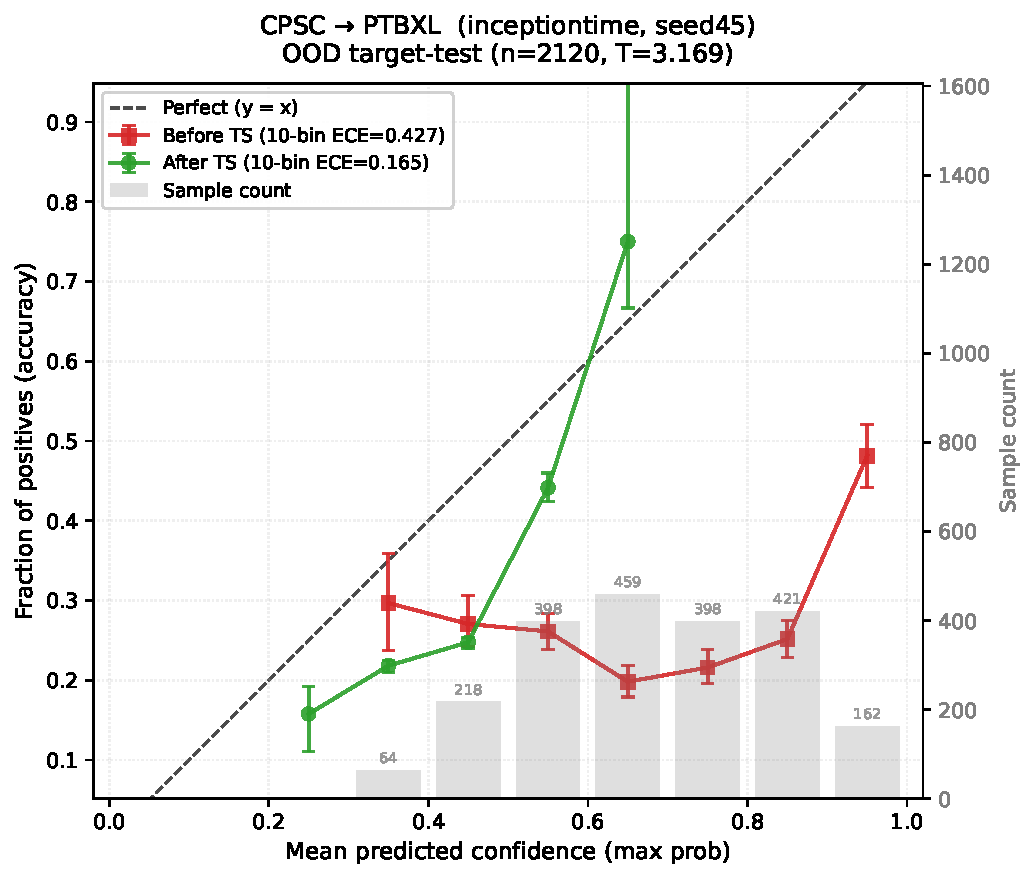
\includegraphics[width=0.45\textwidth]{figures/fig_reliability_supp_cpsc_ptbxl_inceptiontime_seed45.pdf}
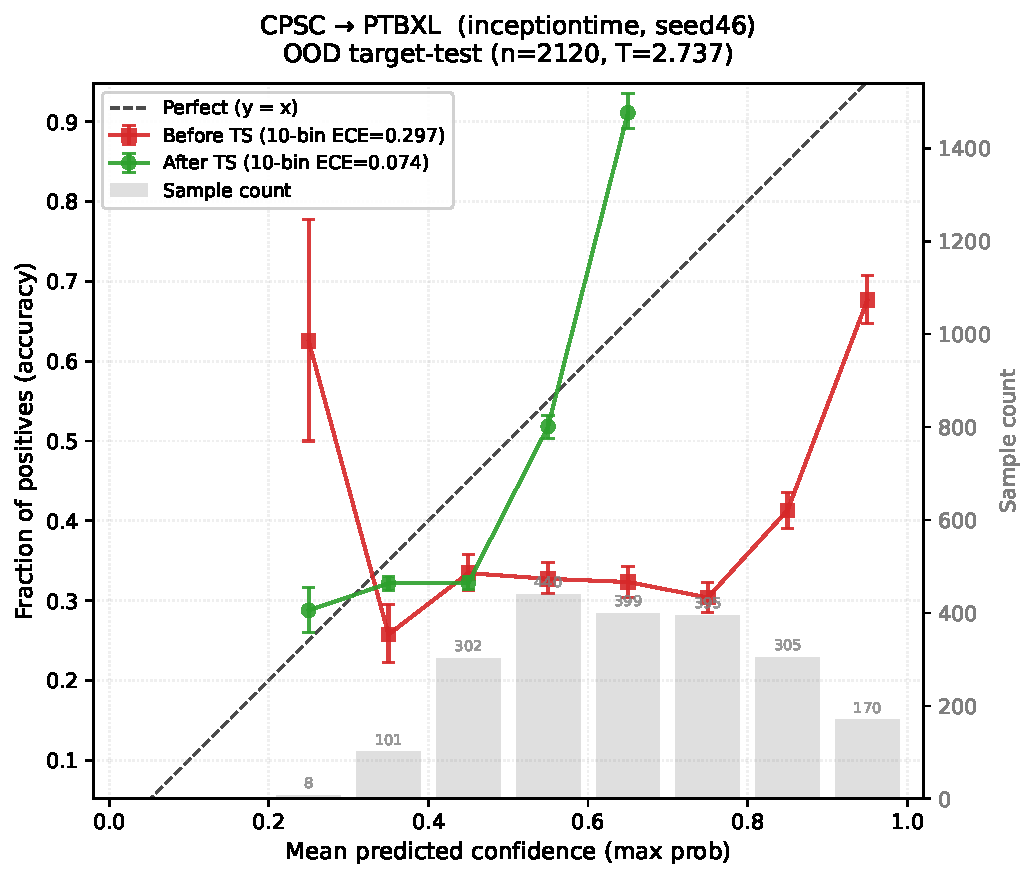
\includegraphics[width=0.45\textwidth]{figures/fig_reliability_supp_cpsc_ptbxl_inceptiontime_seed46.pdf}
\caption{CPSC$\to$PTB-XL reliability diagrams: InceptionTime seeds 45--46.}
\end{figure}

\subsubsection*{S1.5.\ PTB-XL$\rightarrow$Chapman}

\begin{figure}[h]
\centering
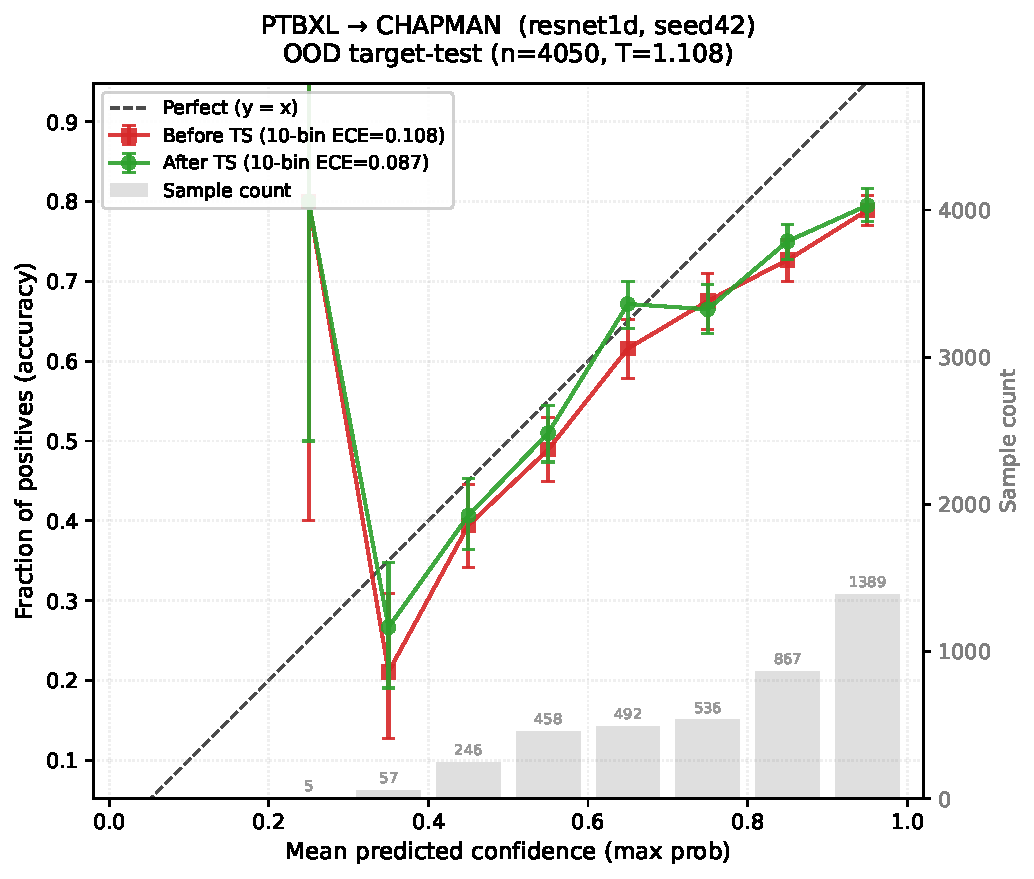
\includegraphics[width=0.32\textwidth]{figures/fig_reliability_supp_ptbxl_chapman_resnet1d_seed42.pdf}
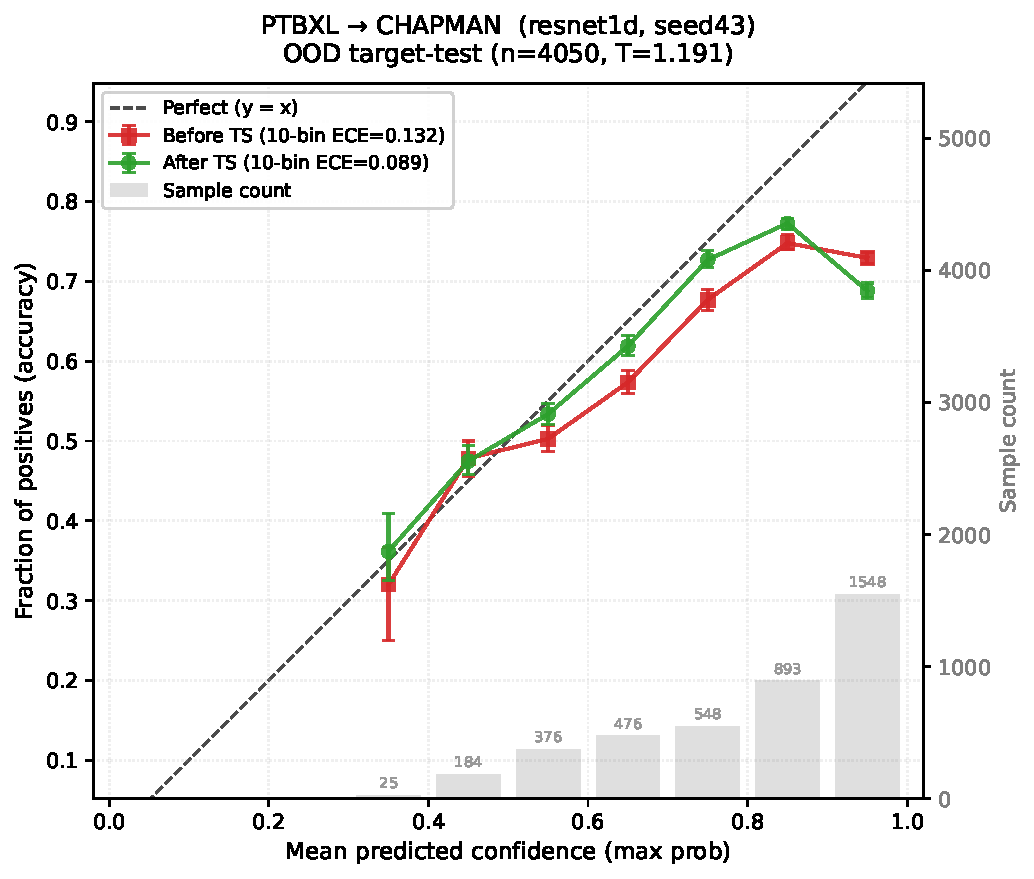
\includegraphics[width=0.32\textwidth]{figures/fig_reliability_supp_ptbxl_chapman_resnet1d_seed43.pdf}
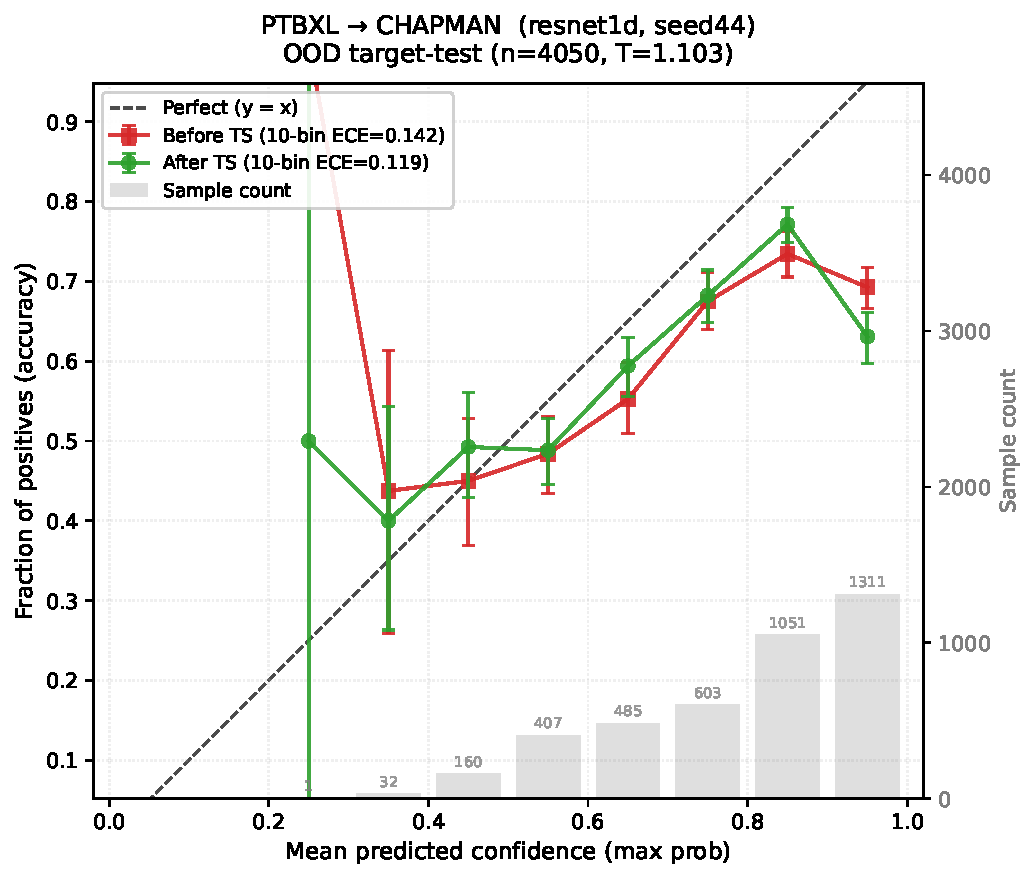
\includegraphics[width=0.32\textwidth]{figures/fig_reliability_supp_ptbxl_chapman_resnet1d_seed44.pdf}
\caption{PTB-XL$\to$Chapman reliability diagrams: ResNet1D seeds 42--44.}
\end{figure}

\begin{figure}[h]
\centering
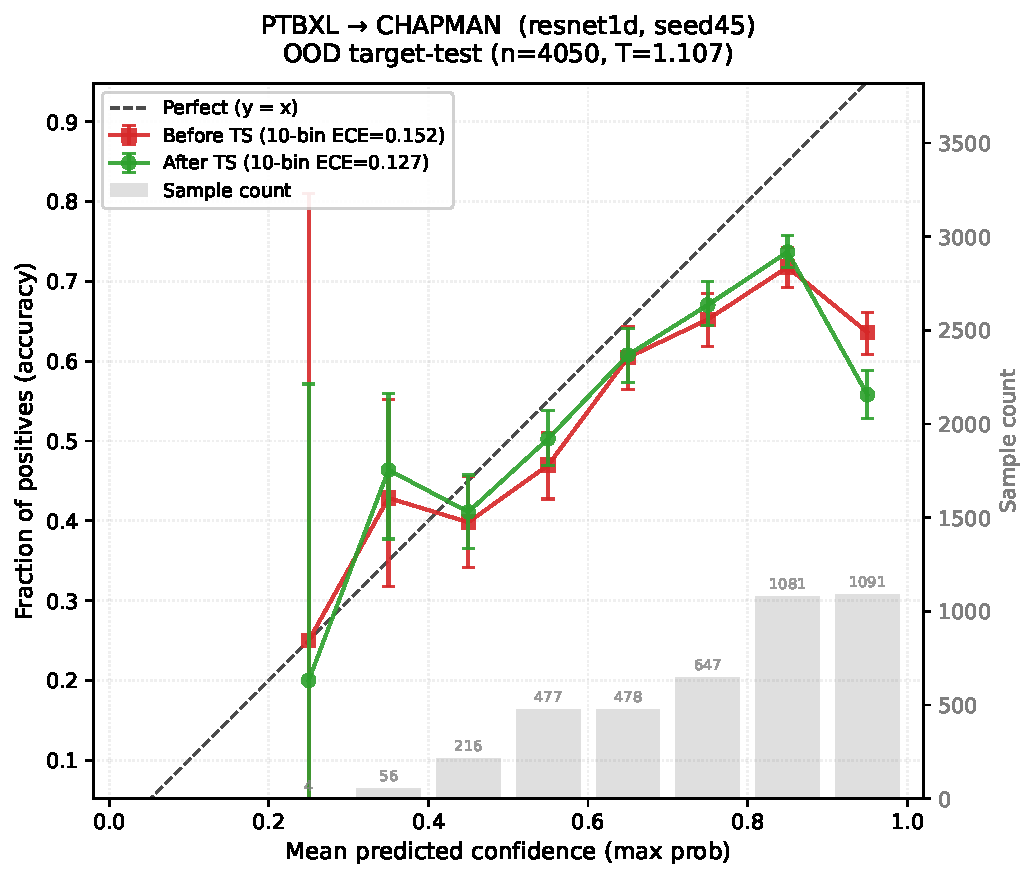
\includegraphics[width=0.45\textwidth]{figures/fig_reliability_supp_ptbxl_chapman_resnet1d_seed45.pdf}
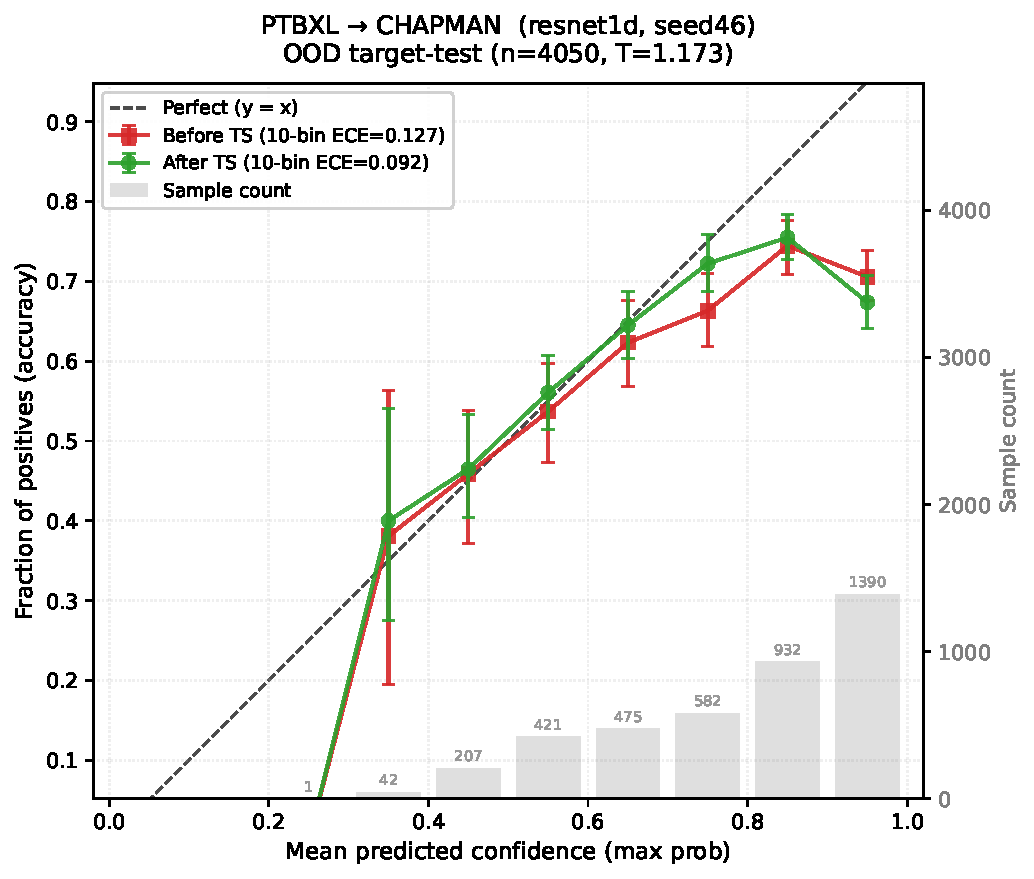
\includegraphics[width=0.45\textwidth]{figures/fig_reliability_supp_ptbxl_chapman_resnet1d_seed46.pdf}
\caption{PTB-XL$\to$Chapman reliability diagrams: ResNet1D seeds 45--46.}
\end{figure}

\begin{figure}[h]
\centering
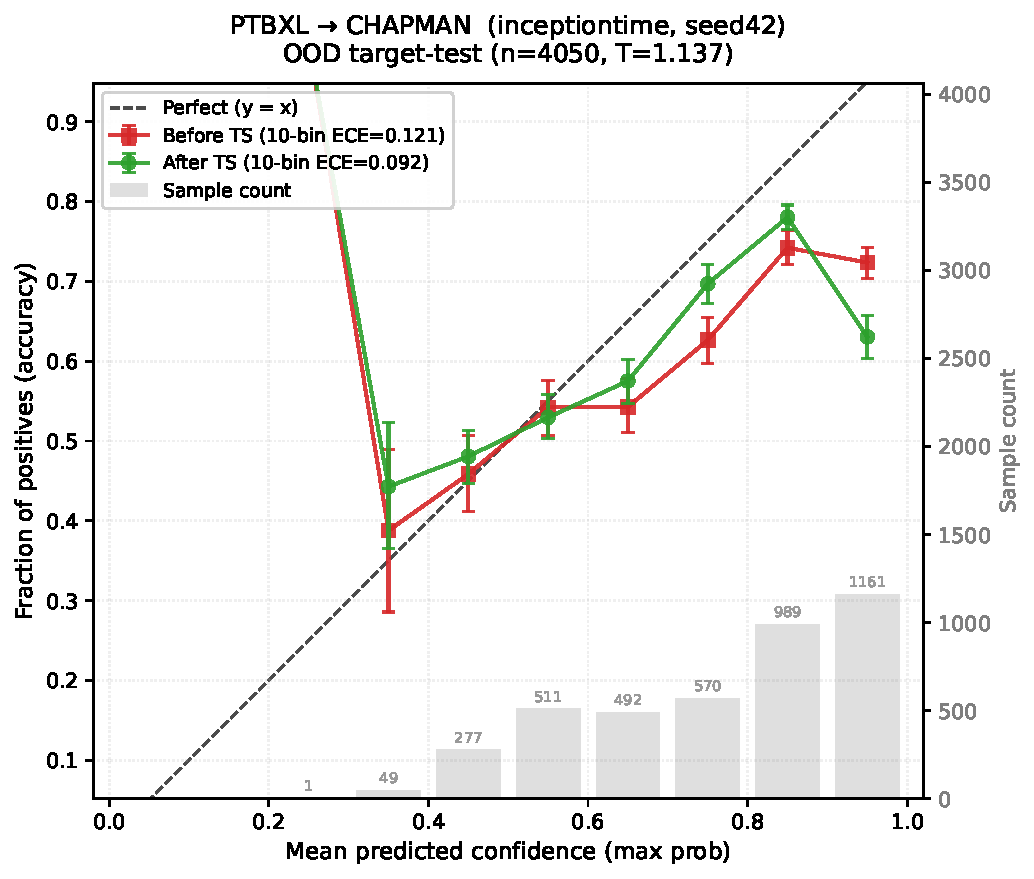
\includegraphics[width=0.32\textwidth]{figures/fig_reliability_supp_ptbxl_chapman_inceptiontime_seed42.pdf}
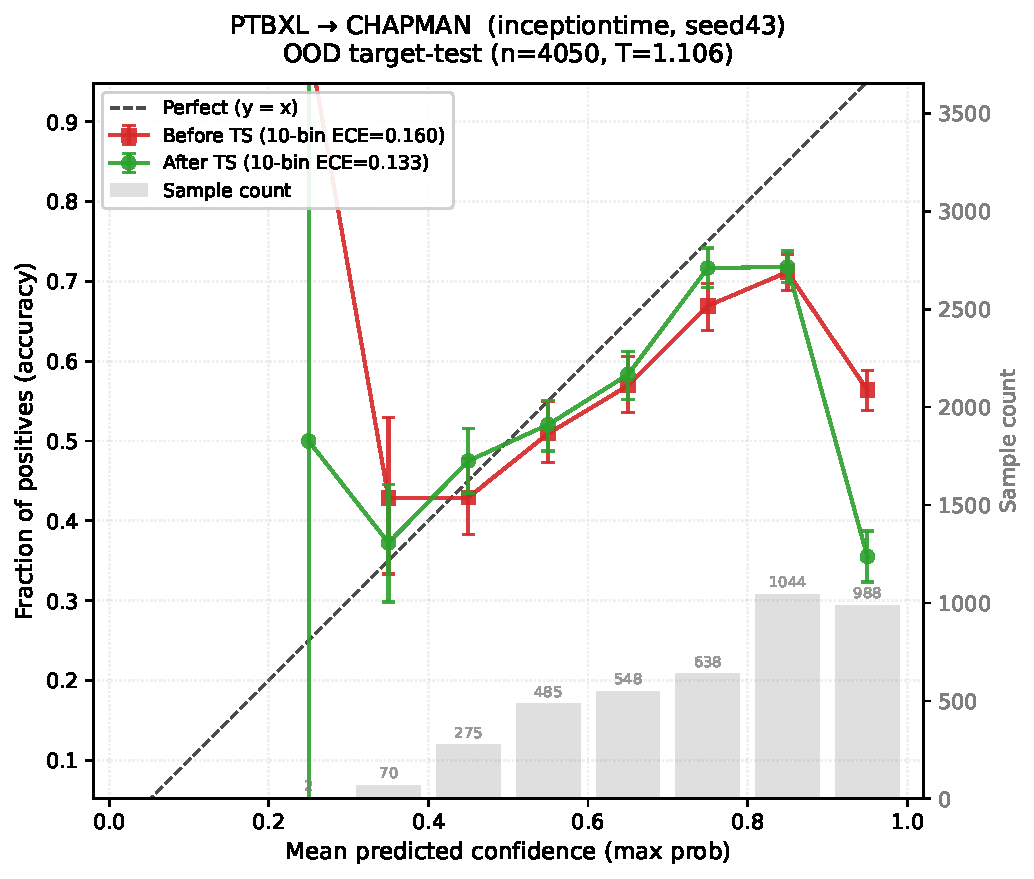
\includegraphics[width=0.32\textwidth]{figures/fig_reliability_supp_ptbxl_chapman_inceptiontime_seed43.pdf}
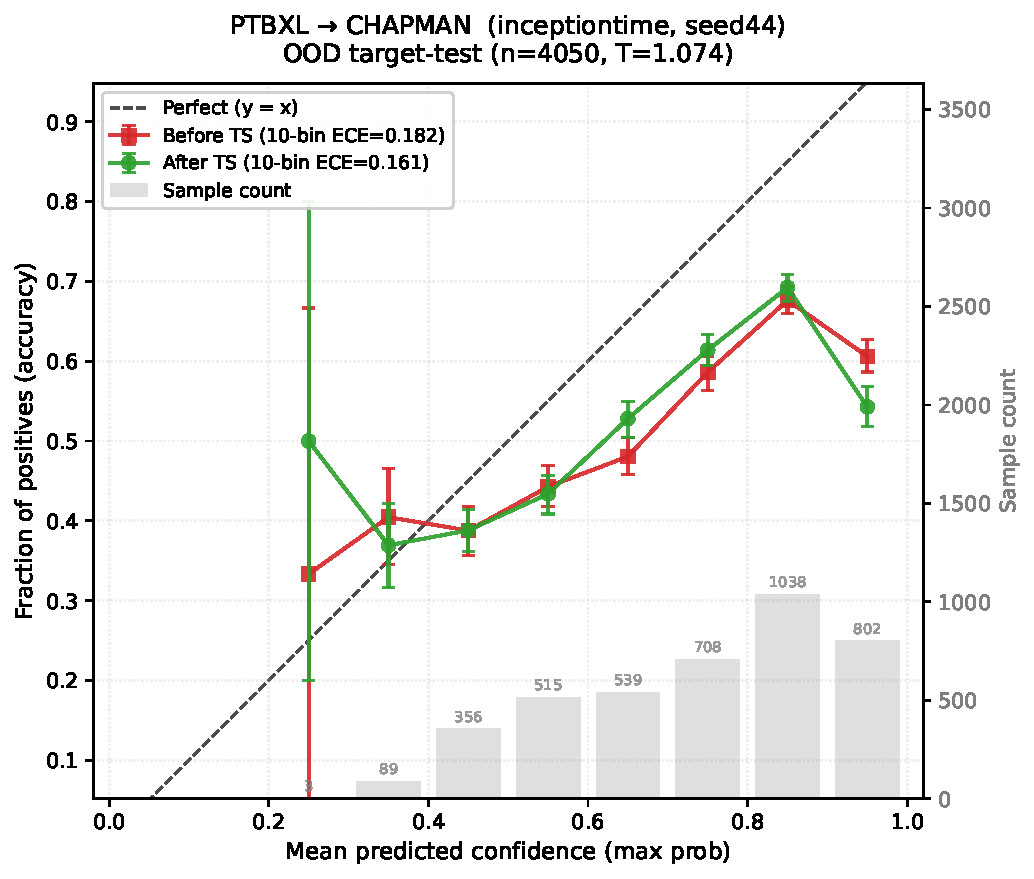
\includegraphics[width=0.32\textwidth]{figures/fig_reliability_supp_ptbxl_chapman_inceptiontime_seed44.pdf}
\caption{PTB-XL$\to$Chapman reliability diagrams: InceptionTime seeds 42--44.}
\end{figure}

\begin{figure}[h]
\centering
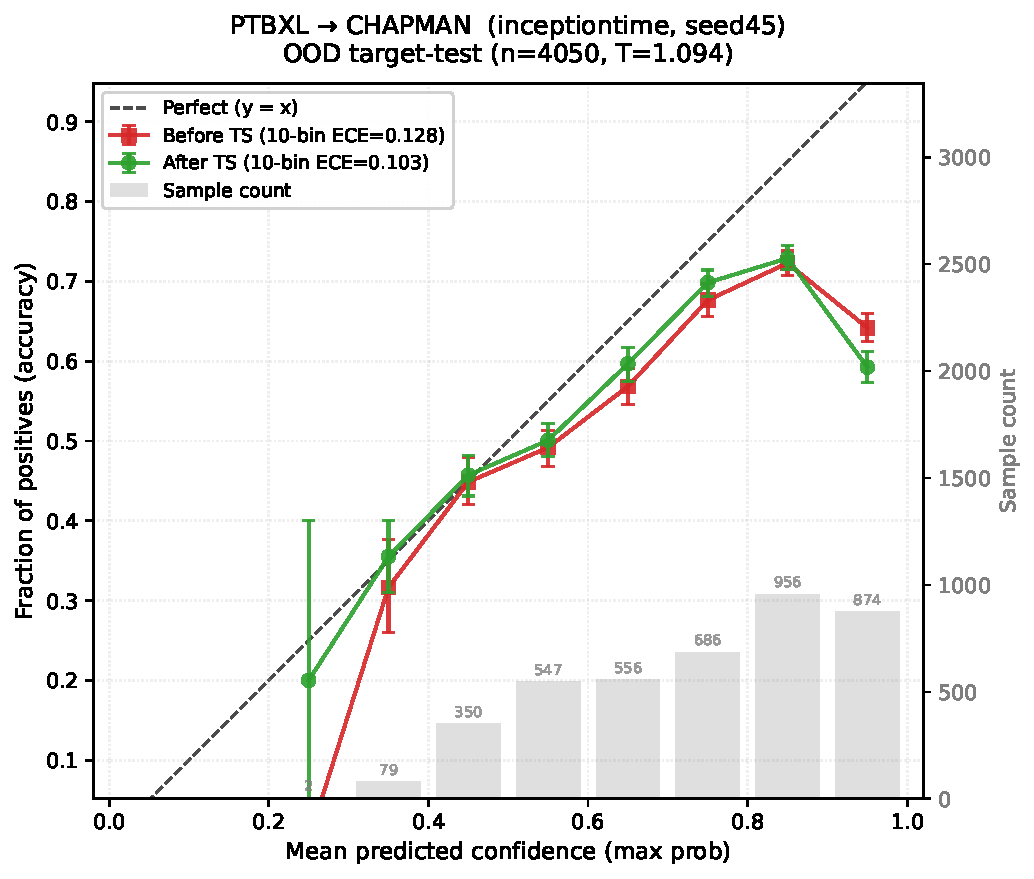
\includegraphics[width=0.45\textwidth]{figures/fig_reliability_supp_ptbxl_chapman_inceptiontime_seed45.pdf}
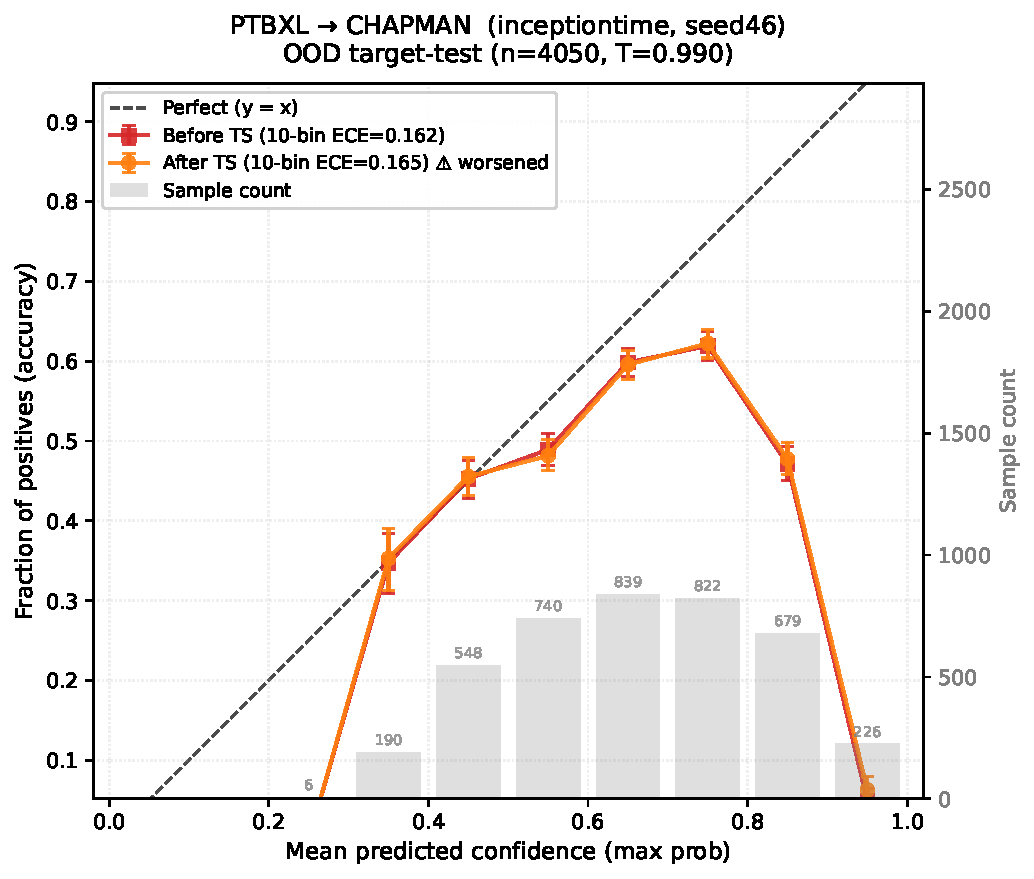
\includegraphics[width=0.45\textwidth]{figures/fig_reliability_supp_ptbxl_chapman_inceptiontime_seed46.pdf}
\caption{PTB-XL$\to$Chapman reliability diagrams: InceptionTime seeds 45--46.}
\end{figure}

\subsubsection*{S1.6.\ PTB-XL$\rightarrow$CPSC}

\begin{figure}[h]
\centering
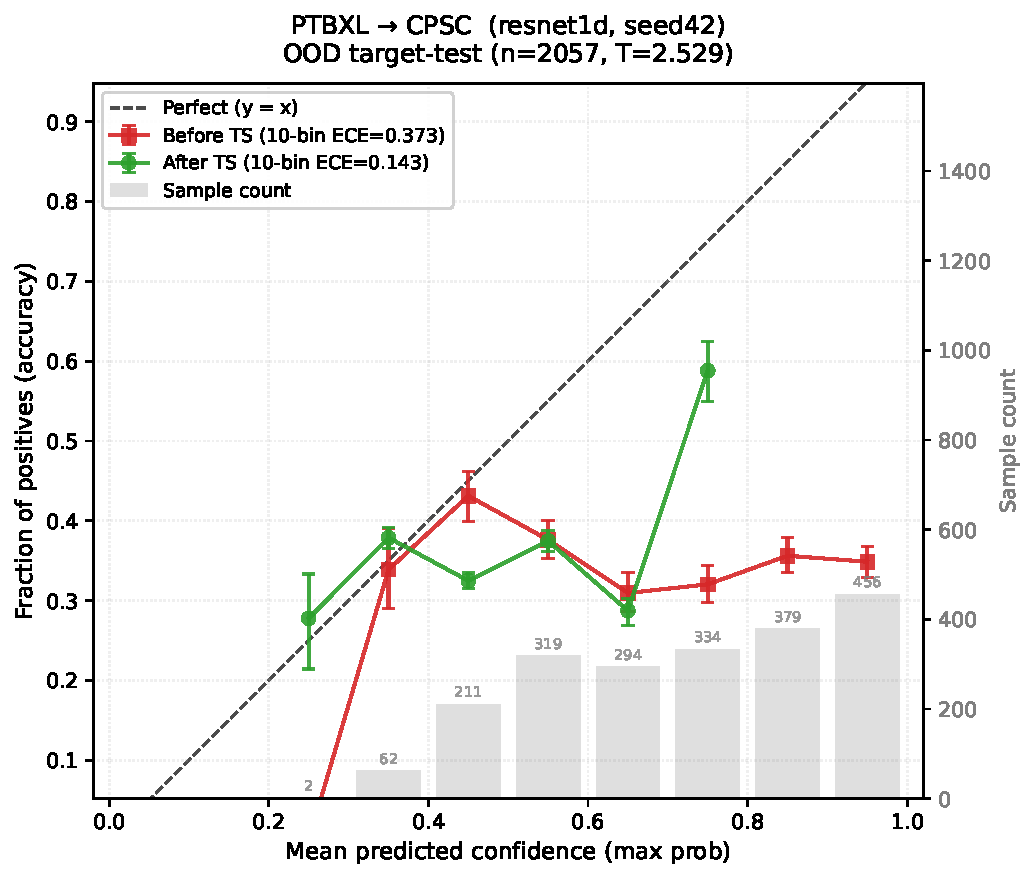
\includegraphics[width=0.32\textwidth]{figures/fig_reliability_supp_ptbxl_cpsc_resnet1d_seed42.pdf}
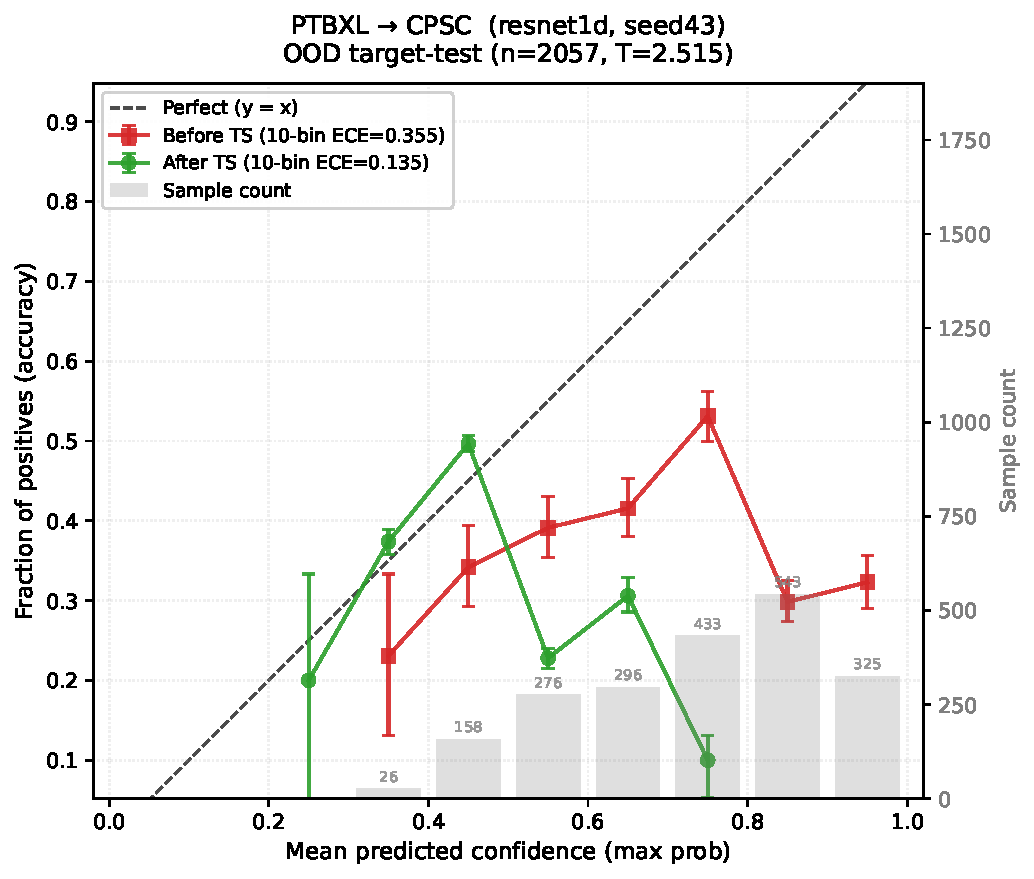
\includegraphics[width=0.32\textwidth]{figures/fig_reliability_supp_ptbxl_cpsc_resnet1d_seed43.pdf}
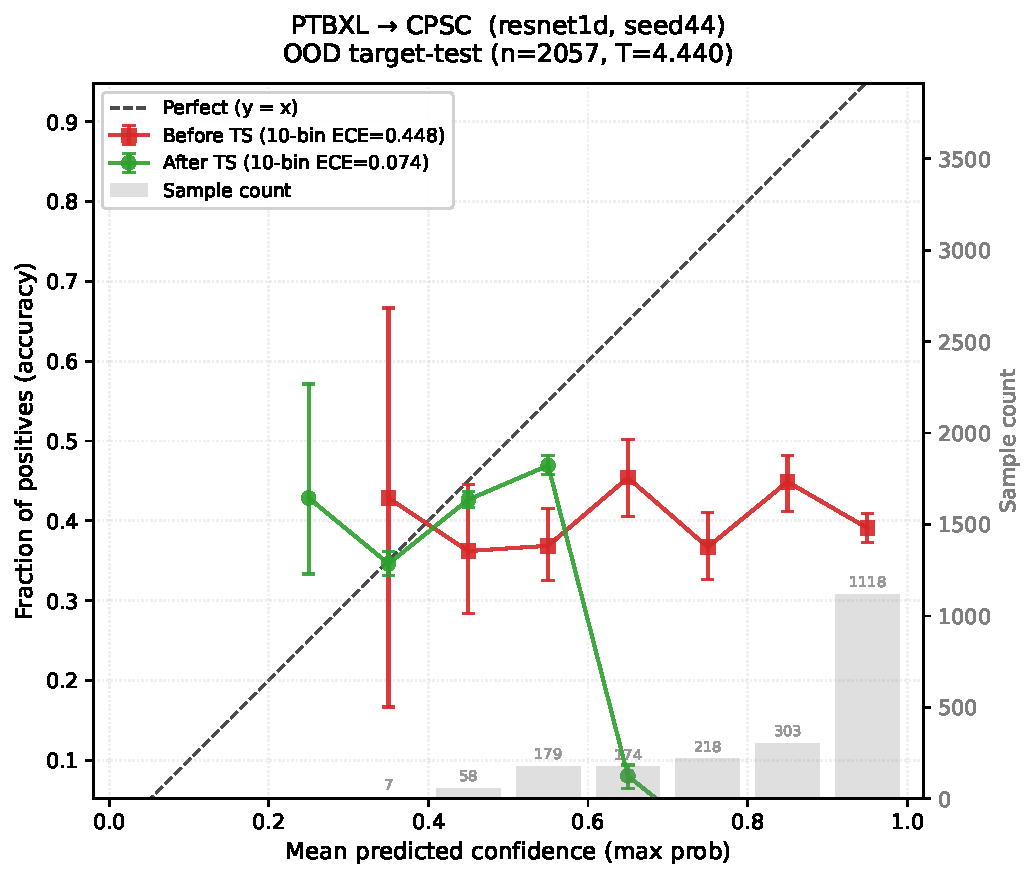
\includegraphics[width=0.32\textwidth]{figures/fig_reliability_supp_ptbxl_cpsc_resnet1d_seed44.pdf}
\caption{PTB-XL$\to$CPSC reliability diagrams: ResNet1D seeds 42--44.}
\end{figure}

\begin{figure}[h]
\centering
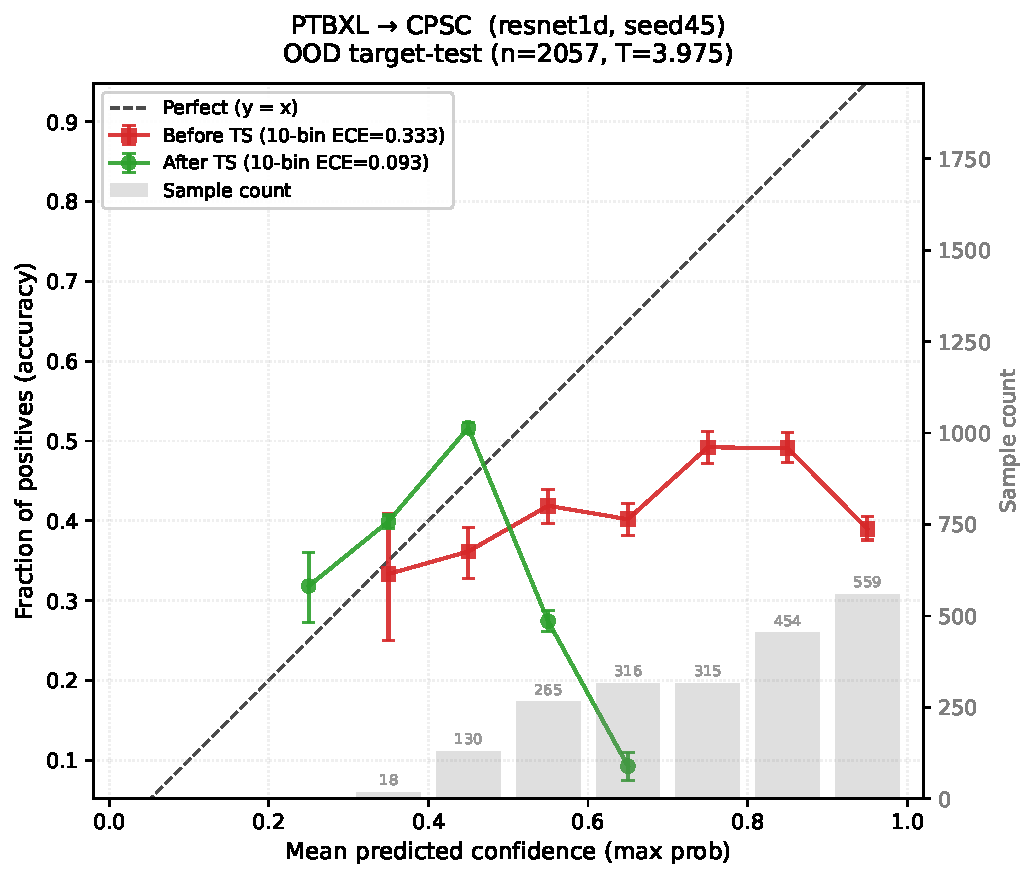
\includegraphics[width=0.45\textwidth]{figures/fig_reliability_supp_ptbxl_cpsc_resnet1d_seed45.pdf}
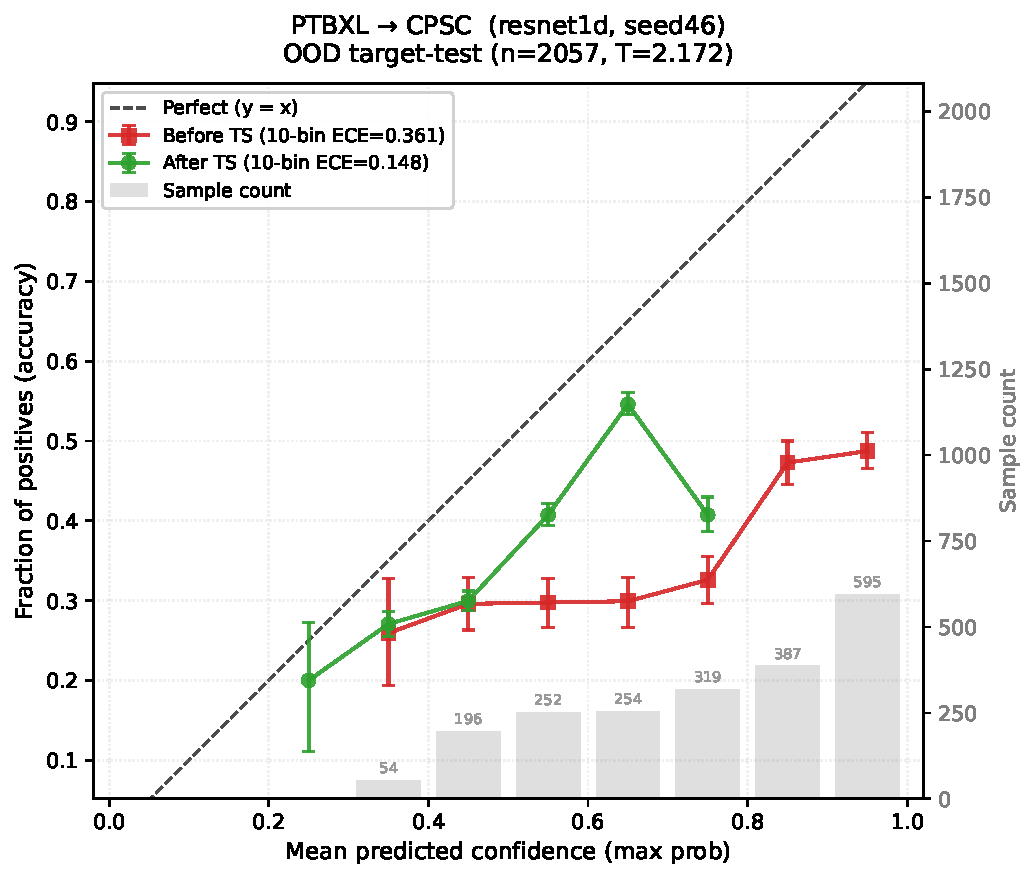
\includegraphics[width=0.45\textwidth]{figures/fig_reliability_supp_ptbxl_cpsc_resnet1d_seed46.pdf}
\caption{PTB-XL$\to$CPSC reliability diagrams: ResNet1D seeds 45--46.}
\end{figure}

\begin{figure}[h]
\centering
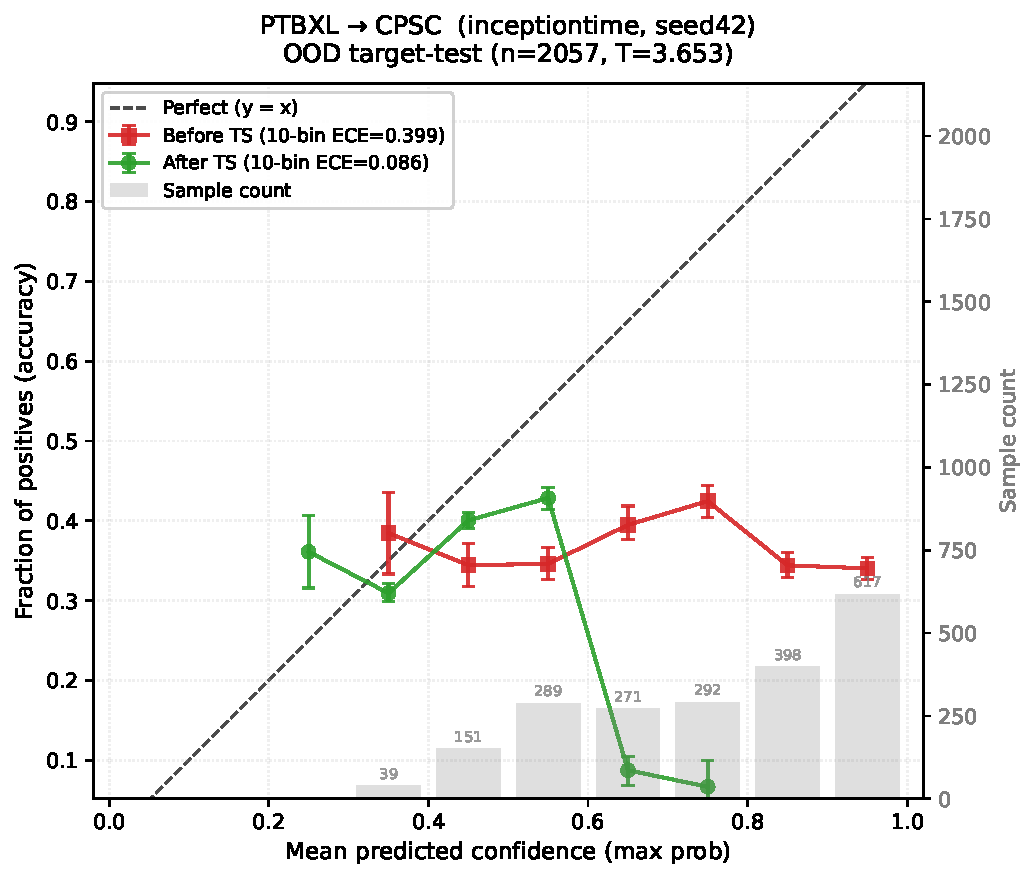
\includegraphics[width=0.32\textwidth]{figures/fig_reliability_supp_ptbxl_cpsc_inceptiontime_seed42.pdf}
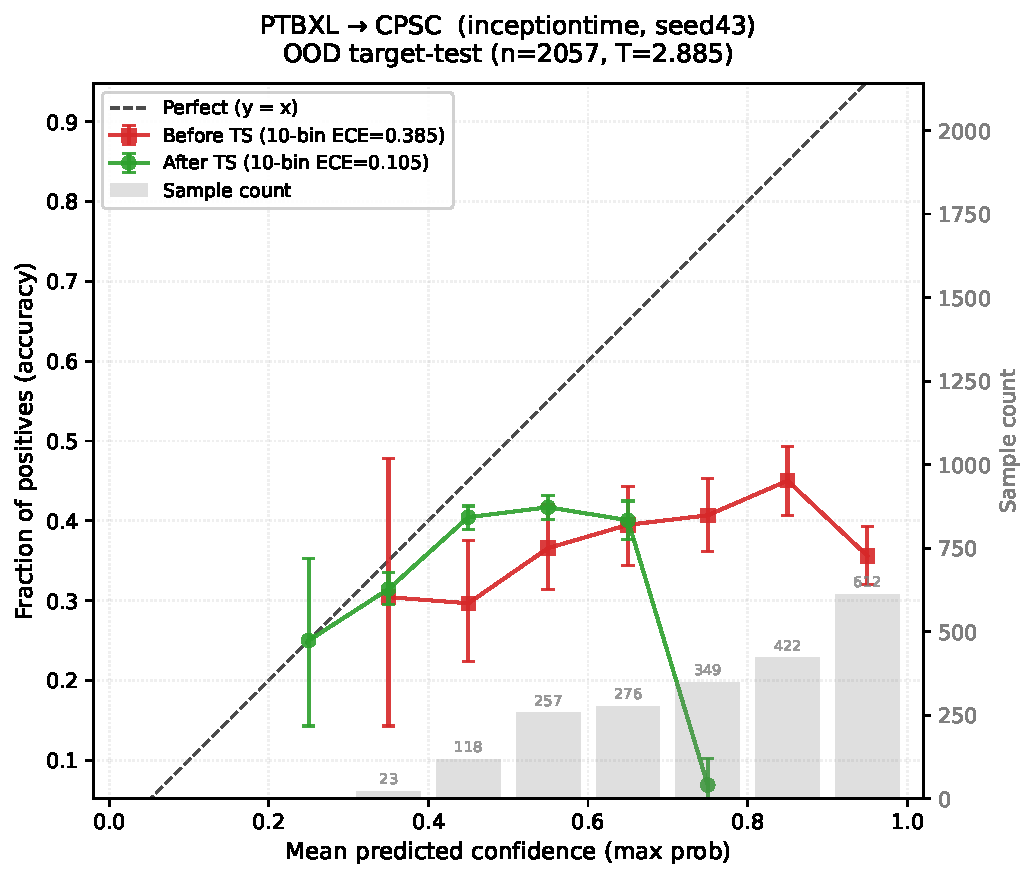
\includegraphics[width=0.32\textwidth]{figures/fig_reliability_supp_ptbxl_cpsc_inceptiontime_seed43.pdf}
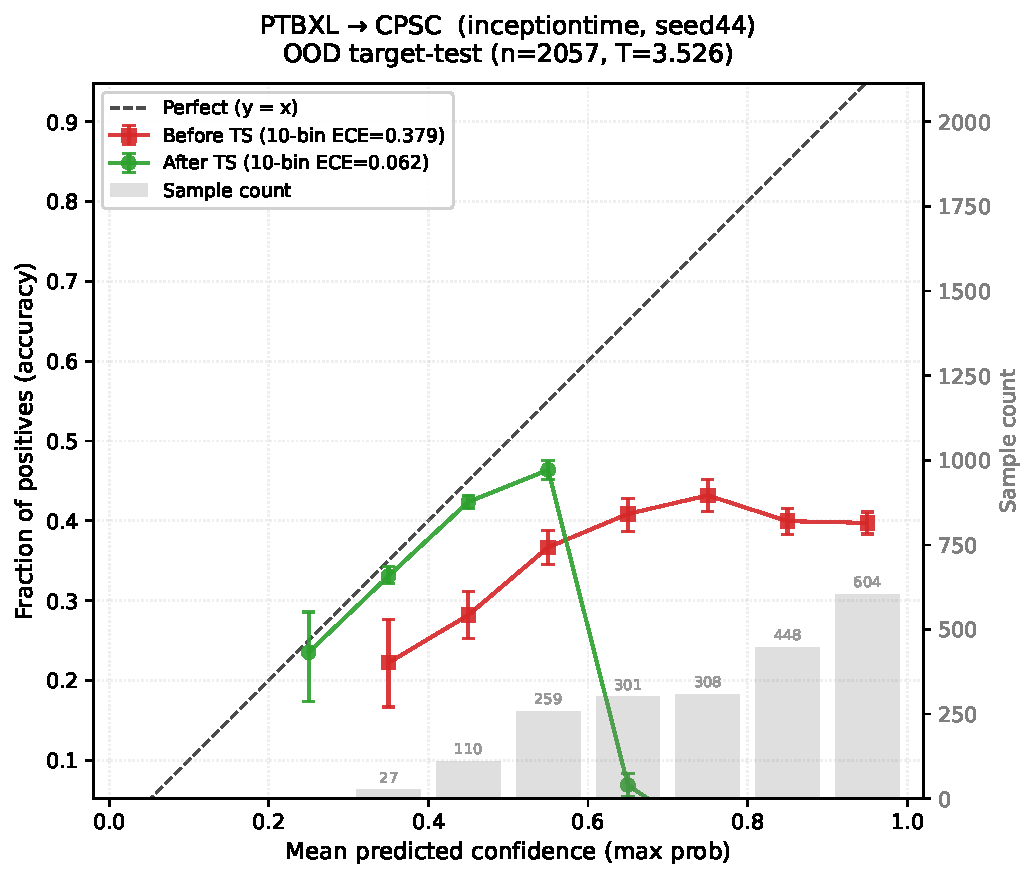
\includegraphics[width=0.32\textwidth]{figures/fig_reliability_supp_ptbxl_cpsc_inceptiontime_seed44.pdf}
\caption{PTB-XL$\to$CPSC reliability diagrams: InceptionTime seeds 42--44.}
\end{figure}

\begin{figure}[h]
\centering
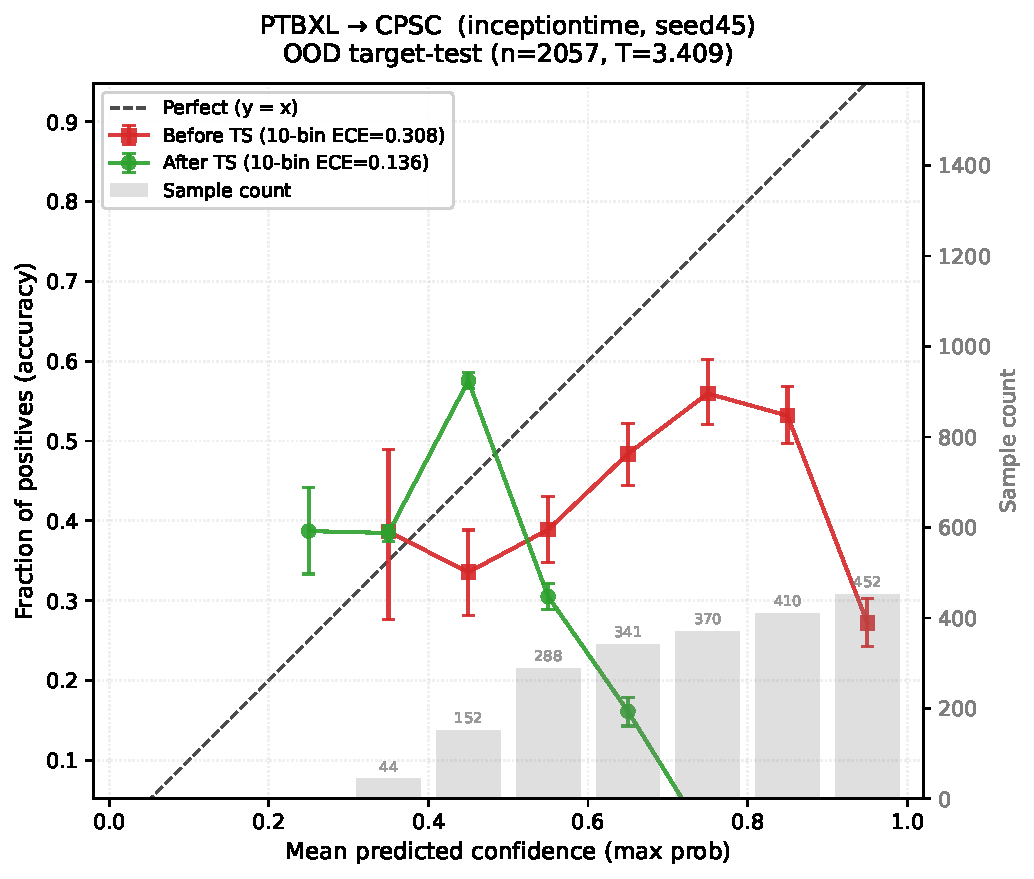
\includegraphics[width=0.45\textwidth]{figures/fig_reliability_supp_ptbxl_cpsc_inceptiontime_seed45.pdf}
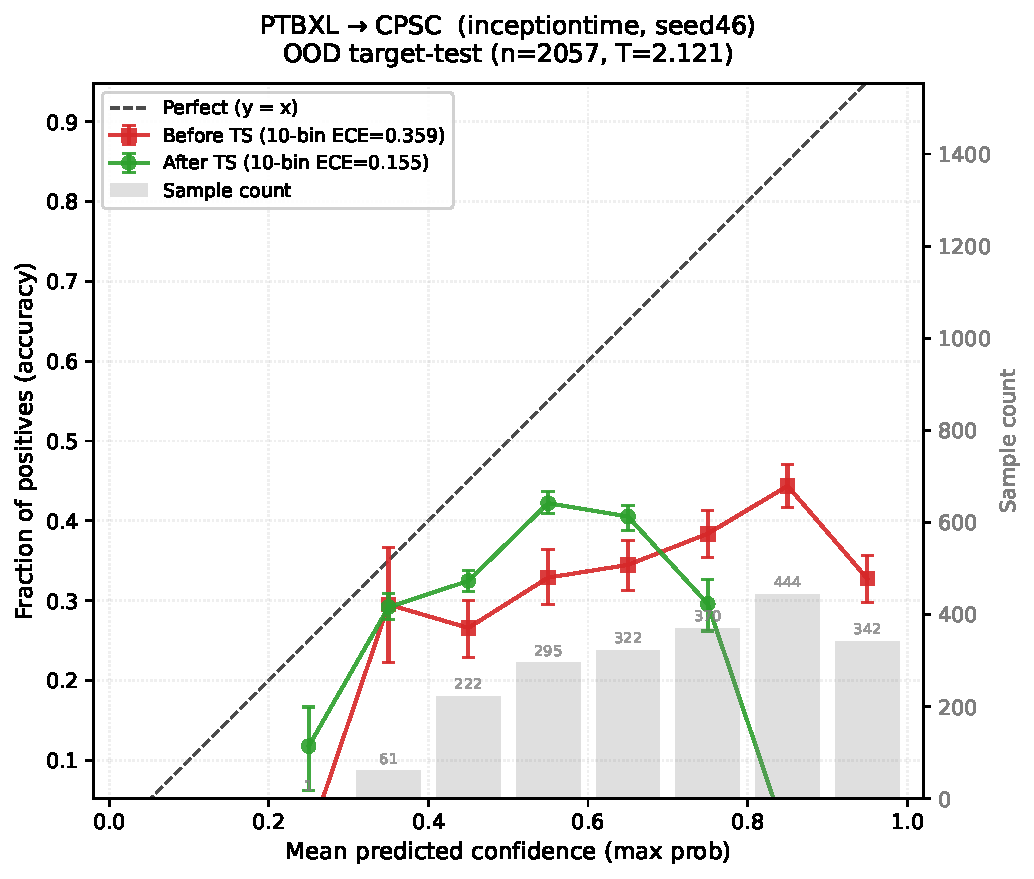
\includegraphics[width=0.45\textwidth]{figures/fig_reliability_supp_ptbxl_cpsc_inceptiontime_seed46.pdf}
\caption{PTB-XL$\to$CPSC reliability diagrams: InceptionTime seeds 45--46.}
\end{figure}

\subsection*{S2.\ Additional supplementary materials}
\label{sec:supp-additional}
\begin{itemize}
    \item \textbf{Per-experiment result files}: full JSON results
    (\texttt{checkpoints/transfer/**/}\allowbreak\texttt{transfer\_result.json})
    and CSV summaries (\texttt{results/*.csv}) for all 60 seed experiments.
    \item \textbf{Pre-registered protocol}: revision A1 full text
    (\texttt{docs/PROTOCOL\_AMENDMENT\_A1\_}\allowbreak\texttt{PREREG\_RELOCATION.md})
    and hash manifest
    (\texttt{docs/osf\_archive\_manifest.json}).
    \item \textbf{NCV experiment data}: E3 CSV containing
    \texttt{ncv\_id} and \texttt{ncv\_ood} columns for the net
    clinical value experiment (Section~\ref{sec:ncv_methods}).
    \item \textbf{Shapley decomposition cells}: 27-cell validation
    table for the Shapley attribution analysis at $n=20{,}000$.
    \item \textbf{BCa CI rerun manifest}: full BCa bootstrap
    ($B=10{,}000$) CI results for the entire $6 \times 2 \times 5
    \times 8$ grid, stored in the \texttt{methods.ts.meta} field of
    each \texttt{transfer\_result.json}.
\end{itemize}

% ============================================================================
\begin{thebibliography}{99}
\raggedright
% ============================================================================
\bibitem{ovadia2019calibration} Y.~Ovadia, E.~Fertig, J.~Ren, Z.~Nado,
D.~Sculley, S.~Nowozin, J.~Dillon, B.~Lakshminarayanan, J.~Snoek,
``Can you trust your model's uncertainty? Evaluating predictive
uncertainty under dataset shift,'' \emph{NeurIPS}, 2019.
arXiv:1906.02530.
\bibitem{guo2017calibration} C.~Guo, G.~Pleiss, Y.~Sun, K.~Weinberger,
``On calibration of modern neural networks,'' \emph{ICML}, PMLR
70:1321--1330, 2017. arXiv:1706.04599.
\bibitem{wagner2020ptbxl} P.~Wagner, N.~Strodthoff, R.-D.~Bousseljot,
et al., ``PTB-XL, a large publicly available electrocardiography
dataset,'' \emph{Scientific Data}, 7:154, 2020.
doi:10.1038/s41597-020-0495-6.
\bibitem{zheng2022ecgarrhythmia} J.~Zheng, J.~Guo, H.~Chu,
``A large scale 12-lead electrocardiogram database for arrhythmia
study (Chapman-Shaoxing e-cardiology),'' version 1.0.0,
\emph{PhysioNet}, 2022. doi:10.13026/wgex-er52.
\bibitem{goldberger2000} A.~L. Goldberger et al., ``PhysioBank,
PhysioToolkit, and PhysioNet: components of a new research resource
for complex physiologic signals,'' \emph{Circulation},
101(23):e215--e220, 2000.
\bibitem{nixon2019} J.~Nixon, M.~W. Dusenberry, L.~Zhang, et al.,
``Measuring calibration in deep learning,'' \emph{CVPR Workshops},
pp.~38--41, 2019. arXiv:1904.01685.
\bibitem{kull2019dirichlet} M.~Kull, M.~Perello-Nieto, M.~Kangse,
T.~S.~Filho, P.~Song, P.~Flach, ``Beyond temperature scaling:
obtaining well-calibrated multi-class probabilities with Dirichlet
calibration,'' \emph{NeurIPS}, 2019. arXiv:1910.12656.
\bibitem{alexandari2020} A.~Alexandari, A.~Kundaje, A.~Shrikumar,
``Maximum likelihood with bias-corrected calibration is hard-to-beat
at label shift adaptation,'' \emph{ICML}, PMLR 119:222--232, 2020.
arXiv:1901.06852.
\bibitem{lipton2018bbs} Z.~Lipton, Y.-X.~Wang, A.~Smola,
``Detecting and correcting for label shift with black box
predictors,'' \emph{ICML}, PMLR 80:1944--1953, 2018.
arXiv:1802.03916.
\bibitem{barandas2023} M.~Barandas, L.~Famiglini, A.~Campagner,
D.~Folgado, R.~Sim\~ao, F.~Cabitza, H.~Gamboa, ``Evaluation of
uncertainty quantification methods in multi-label classification: a
case study with automatic diagnosis of electrocardiogram,''
\emph{Information Fusion}, 101:101978, 2024.
doi:10.1016/j.inffus.2023.101978.
\bibitem{zhang2022} J.~F.~Vranken et al., ``Uncertainty estimation for
deep learning-based automated analysis of 12-lead
electrocardiograms,'' \emph{European Heart Journal -- Digital Health},
2(3):423--434, 2021. doi:10.1093/ehjdh/ztab045.
\bibitem{reyna2022} M.~Reyna, N.~Strodthoff, P.~Wagner, et al.,
``Issues in the automated classification of multilead ECGs using
heterogeneous labels and populations,'' \emph{Physiological
Measurement}, 43(8):084001, 2022. doi:10.1088/1361-6579/ac79fd.
\bibitem{efron1987bca} B.~Efron, ``Better bootstrap confidence
intervals,'' \emph{Journal of the American Statistical Association},
82(397):171--185, 1987. doi:10.1080/01621459.1987.10478410.
\bibitem{vancalster2016} B.~Van Calster, D.~J.~Steyerberg,
S.~Collins, R.~D.~Riley, E.~W.~Steyer, ``A calibration hierarchy for
risk models was defined: from utopia to empirical data,''
\emph{Journal of Clinical Epidemiology}, 74:167--176, 2016.
doi:10.1016/j.jclinepi.2015.12.005.
\bibitem{vancalster2019} B.~Van Calster, D.~J.~McLernon,
M.~van~Smeden, L.~Wynants, G.~S.~Collins, ``Calibration: the Achilles
heel of predictive analytics,'' \emph{BMC Medicine}, 17:230, 2019.
doi:10.1186/s12916-019-1466-7.
\bibitem{kumar2019} A.~Kumar, P.~Liang, T.~Ma, ``Verified uncertainty
calibration,'' \emph{NeurIPS}, 2019. arXiv:1909.10155.
\bibitem{strodthoff2021} N.~Strodthoff, P.~Wagner, T.~Schaeffter,
W.~Samek, ``Deep learning for ECG analysis: benchmarks and insights
from PTB-XL,'' \emph{IEEE Journal of Biomedical and Health
Informatics}, 25(5):1519--1528, 2021.
doi:10.1109/JBHI.2020.3022989.
\bibitem{physiolmeas2026} M.~Haekal, S.~N.~Khotimah,
G.~R.~F.~Suwandi, F.~Haryanto, ``RR-interval-based atrial fibrillation
detection and burden estimation: cross-dataset validation and
calibration-aware probability analysis,'' \emph{Physiological
Measurement}, 2026. doi:10.1088/1361-6579/ae99aa.
\bibitem{medrxiv2026} K.~Patel, P.~Beedala, ``Calibration drift under
cross-institutional deployment: an external validation framework for
ICU mortality prediction across MIMIC-IV and eICU,'' \emph{medRxiv}
(preprint), 2026. doi:10.64898/2026.05.03.26352335.
\bibitem{transcal2020} X.~Wang, M.~Long, J.~Wang, M.~I.~Jordan,
``TransCal: transferability estimation for auto-selecting transfer
calibration,'' \emph{NeurIPS}, 2020. arXiv:2007.08259.
\bibitem{pseudocal2020} S.~Garg, Y.~Wu, S.~Balakrishnan, Z.~Lipton,
``A unified view of label shift estimation,'' \emph{NeurIPS}, 2020.
arXiv:2003.07554.
\bibitem{lascal2024} T.~Popordanoska, G.~Radevski, T.~Tuytelaars, et al.,
``LaSCal: label-shift calibration for uncertainty quantification,''
\emph{NeurIPS}, 2024.
\bibitem{morenotorres2012} J.~T.~Moreno-Torres, T.~Raeder,
R.~Alaiz-Rodriguez, N.~Chawla, F.~Herrera, ``A unifying view on
dataset shift in classification,'' \emph{Pattern Recognition},
45(1):521--530, 2012. doi:10.1016/j.patcog.2011.05.019.
\bibitem{protocolv21a1} [Unpublished pre-registered protocol] ``ECG
calibration boundary study -- pre-registered experiment protocol
v2.1-A1,'' 2026. Hash manifest:
\texttt{docs/osf\_archive\_manifest.json} (local snapshot; public OSF
archival pending); revision A1 full text in
\texttt{docs/PROTOCOL\_AMENDMENT\_A1\_PREREG\_RELOCATION.md}.
\bibitem{nosek2019prereg} B.~Nosek, C.~Ebersole, A.~DeHaven,
D.~Mellor, ``The preregistration revolution,'' \emph{PNAS},
115(11):2600--2606, 2018. doi:10.1073/pnas.1708274114.
\bibitem{lakens2019prereg} D.~Lakens, ``The practical alternative to
the $p$ value is the correctly used $p$ value,''
\emph{Perspectives on Psychological Science}, 16(3):639--648, 2021.
doi:10.1177/1745691620958012.
\bibitem{ecgfounder2024} J.~Li, A.~D.~Aguirre, V.~M.~Junior, et al.,
``An Electrocardiogram Foundation Model Built on over 10 Million
Recordings,'' \emph{NEJM AI},
2(7):AIoa2401033, 2025. doi:10.1056/AIoa2401033.
\bibitem{ecgfm2024} J.~C.~McHugh, B.~Wang, et al., ``ECG-FM: an open
electrocardiogram foundation model,'' \emph{arXiv preprint}
2408.05178, 2024.
\bibitem{heartlang2025} J.~Jin, et al., ``Reading your heart: learning
ECG words and sentences via pre-training ECG language model
(HeartLang),'' \emph{ICLR}, 2025. arXiv:2502.10707.
\bibitem{transferecg2025} C.~V.~Nguyen, C.~D.~Do, ``Transfer learning in ECG
diagnosis: is it effective?'' \emph{PLOS ONE}, 20(5):e0316043, 2025.
doi:10.1371/journal.pone.0316043.
\bibitem{adaptood2026} S.~Vavaroutas, et al., ``ADAPTOOD:
uncertainty-aware fine-tuning for out-of-distribution ECG time series
models,'' \emph{arXiv preprint} 2606.04164, 2026.
\bibitem{beatrhythm2026} W.~Jiang, et al., ``Test-time adaptation for ECG
classification via SQI-gated self-training and beat-rhythm
consistency,'' \emph{arXiv preprint} 2608.23347, 2026 (accepted at
MICCAI 2026).
\bibitem{star2025} N.~Nemati, ``Comparative analysis of data
augmentation for clinical ECG classification with STAR (Sinusoidal
Time--Amplitude Resampling),'' \emph{arXiv preprint} 2510.24740, 2025.
\bibitem{peace2026} X.~Liu, et al., ``PEACE: knowledge-guided
cross-modal fusion for adult-to-pediatric ECG transfer via
label-conditioned contrastive alignment,'' \emph{arXiv preprint}
2605.00647, 2026.
\bibitem{song2024ecgfm} J.~Song, J.-H.~Jang, B.~T.~Lee, D.~Hong,
J.~Kwon, Y.-Y.~Jo, ``Foundation models for electrocardiograms,''
\emph{arXiv preprint} 2407.07110, 2024.
\end{thebibliography}

\end{document}
